%\input{sections/martian-environment/references.tex}

\section{Seasons}
\label{sec:MartianEnvironment:Seasons}
The red planet's axis is tilted away from the sun at \SI{25}{\degree}. Very much like Earth's \SI{23.5}{\degree} axial tilt, this results in seasons. Mars has an orbit with a semi-major axis of \SI{1.524}{\astronomicalunit} which translates to a Martian year corresponding to an orbital period of 687 days. Martian seasons are longer and for every Martian year 1.88 Earth years go by. Sidereal days are 24.62 hours long and solar days are 24.65 hours long. A Martian day, known as a Sol, is approximately 40 minutes longer than an Earth day. Mars' position on its orbit is described in terms of areocentric longitude of the Sun, $L_{s}$, and is measured Eastwards from $L_{s} = \SI{0}{\degree}$ at the northern hemisphere's Vernal equinox. The transition of Martian seasons are presented in Table \ref{tab:mars-seasonal-advances} with respect to areocentric longitudes.

\begin{table}[H]
  \centering
  \caption{Seasonal advances on Mars.}
  \label{tab:mars-seasonal-advances}
  \begin{tabular}{|l|l|l|}
  \hline
  \multirow{2}{*}{\textbf{\begin{tabular}[c]{@{}l@{}}Areocentric\\ Longitude\end{tabular}}} & \multicolumn{2}{c|}{\textbf{Seasonal Advance}} \\ \cline{2-3}
   & \multicolumn{1}{c|}{\textbf{Northern Hemisphere}} & \multicolumn{1}{c|}{\textbf{Southern Hemisphere}} \\ \hline
  \textbf{\si{0}{\degree}} & Vernal Equinox & Autumnal Equinox \\ \hline
  \textbf{\si{0}{\degree} to \si{90}{\degree}} & Spring & Autumn \\ \hline
  \textbf{\si{90}{\degree}} & Summer Solstice & Winter Solstice \\ \hline
  \textbf{\si{90}{\degree} to \si{180}{\degree}} & Summer & Winter \\ \hline
  \textbf{\si{180}{\degree}} & Autumnal Equinox & Vernal Equinox \\ \hline
  \textbf{\si{180}{\degree} to \si{270}{\degree}} & Autumn & Spring \\ \hline
  \textbf{\si{270}{\degree}} & Winter Solstice & Summer Solstice \\ \hline
  \textbf{\si{270}{\degree} to \si{360}{\degree}} & Winter & Summer \\ \hline
  \end{tabular}
\end{table}



\section{Dust}
\label{sec:MartianEnvironment:Dust}
The Martian surface is aeolianly active with varying concentration of airborn dust throughout the year due to processes of dust lifting, transportation, and deposition \citemarsenv{Kahre2006}.

\todo[inline]{TODO: Spice up this intro.}

\subsection{Atmospheric Opacity}
\label{sec:MartianEnvironment:Dust:AtmosphericOpacity}
The density of suspended dust determines the atmospheric opacity, or optical depth, measured in $\tau$ factors. A $\tau$ factor between 0 and 0.5 indicates a clear to relatively clear day. Higher $\tau$ factors indicate dusty days with growing atmospheric dust opacity as represented in Figure \ref{fig:image:tau-factors} for simulated views pointing towards the Sun. \SI{99}{\percent} of sunlight is blocked at $\tau$ factor 4.7.

\todo[inline]{TODO: Source the 99\% claim.}

\begin{figure}[H]
  \centering
  \hypersetup{linkcolor=captionTextColor}
  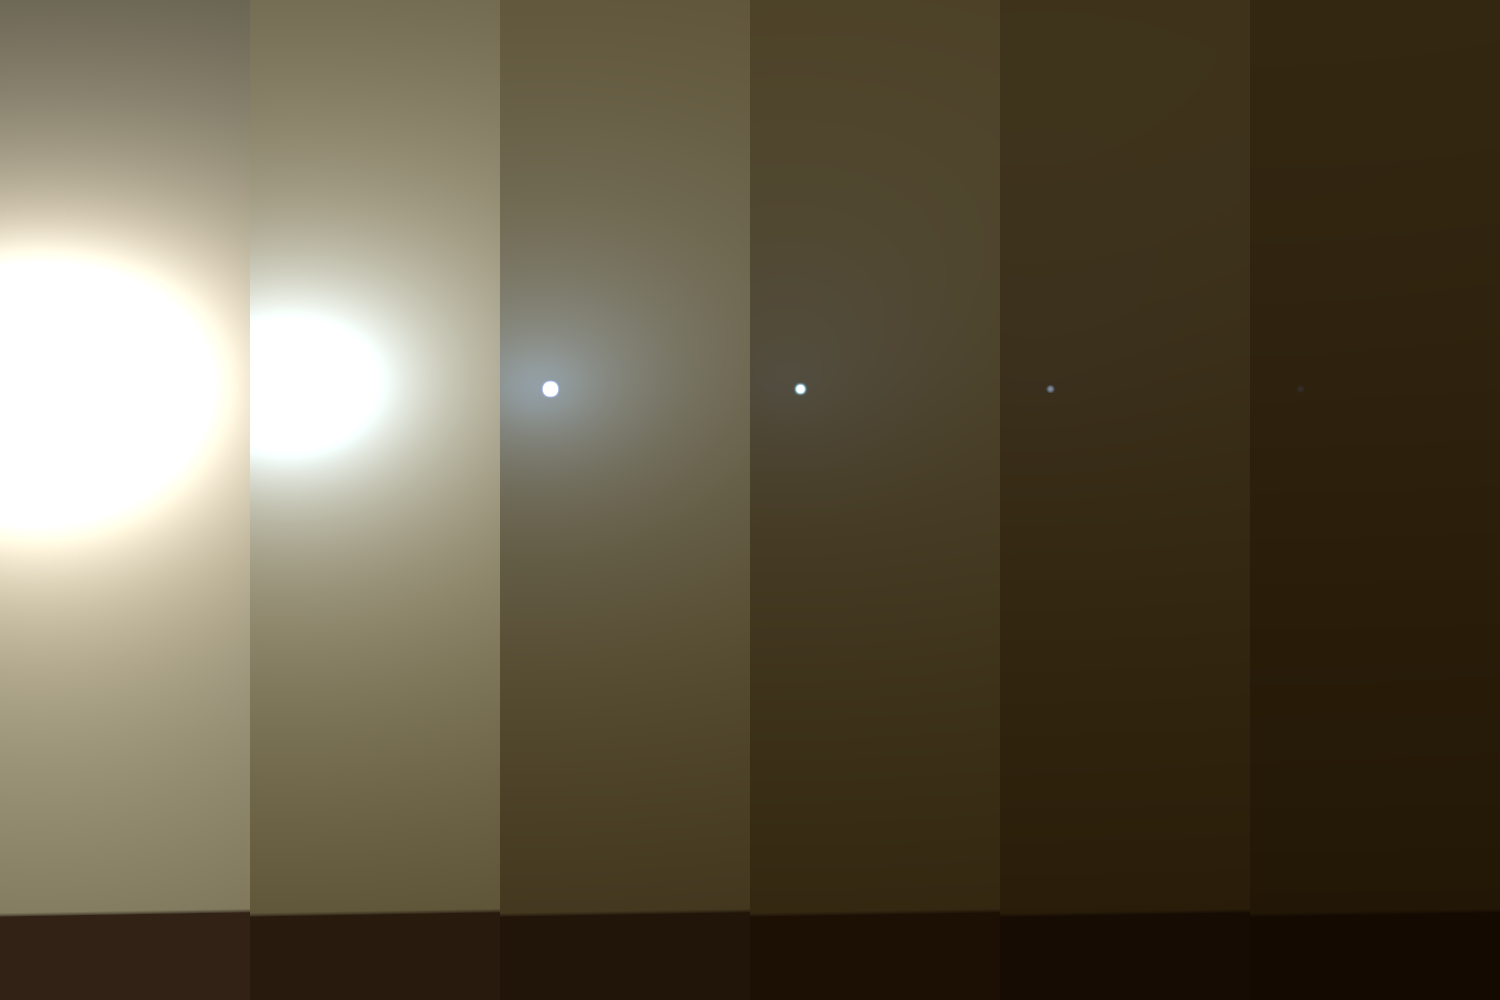
\includegraphics[width=0.8\linewidth]{sections/martian-environment/images/tau-factors.png}\\
  \caption[Simulated views of atmospheric dust opacity for varying $\tau$ factors]
          {Simulated views of atmospheric dust opacity for varying $\tau$ factors. From left to right frames, tau factors of 1, 3, 5, 7, 9, and 11. Credits: NASA/JPL-Caltech/TAMU.}
  \label{fig:image:tau-factors}
\end{figure}

\subsection{Storms}
\label{sec:MartianEnvironment:Dust:Storms}

Dust storms are likely to occur between $L_{s} = \SI{180}{\degree}$ and $L_{s} = \SI{330}{\degree}$ while Mars approaches the Sun, with the perihelion at $L_{s} = \SI{248}{\degree}$. The Sun's proximity warms the atmosphere which creates temperature differences that produce dust lifting winds. The process is exacerbated by the release of carbon dioxide from the evaporating winter polar cap which thickens the atmosphere and increases surface pressure so that dust particles remain airborn.

% Source: https://www.nasa.gov/feature/goddard/2018/curiosity-photos-show-martian-dust-storm-growing

Global dust storms that cover an area of over \SI{e7}{\kilo\meter\squared} have a yearly probability of \SI{30}{\percent} to \SI{80}{\percent} whereas local dust storms that cover an area less than \SI{e7}{\kilo\meter\squared} occur with a \SI{5}{\percent} probability \citepower{Kerslake1999}. Local dust storms typically have a $\tau$ factor of approximately 1 \citepower{Kerslake1999} whereas the largest in situ $\tau$ factor recorded by MER Opportunity was 10.8 on Sol 5111 at $L_{s} = \SI{180}{\degree}$.


\section{Solar Radiation}
\label{sec:MartianEnvironment:SolarRadiation}

\todo[inline]{TODO: Short introduction on Solar Radiation}

The radiation profiles illustrated in this section with respect to Martian surface are for MER Opportunity's final location at Endeavour Crater. Calculations presented in this section as well their nomenclatures are taken from \citemarsenv{Appelbaum1989}, \citemarsenv{Appelbaum1990}, \citemarsenv{Appelbaum1991}, \citemarsenv{Appelbaum1993}, and \citemarsenv{Appelbaum1994} where profiles at locations of Viking Landers VL1 and VL2 can be observed.

\subsection{Irradiance}
\label{sec:MartianEnvironment:SolarRadiation:Irradiance}

Beam irradiance is the total solar flux density expressed in \si{\watt\per\meter\squared}. It is a measure of solar radiation from direct sunlight. At the top of the Martian atmosphere the instantaneous beam irradiance, $G_{ob}$, is a function the areocentric longitude $L_{s}$:

\begin{equation}
  \label{eq:G_ob}
  G_{ob} = 590 \frac{[1 + e \cos{(Ls - 248)}]^2}{(1-e^2)^2}
\end{equation}

Where \SI{590}{\watt\per\meter\squared} is the mean beam irradiance at the top of the Martian atmosphere, $L_{s} - \SI{248}{\degree}$ is the true anomaly, and $e$ is the Mars eccentricity. The variation of $G_{ob}$ is presented in Figure \ref{fig:plot:beam-irradiance-top-of-mars-atmosphere}. At its closest, the perihelion, Mars is at a distance of \SI{1.381}{\astronomicalunit} from the Sun with a beam irradiance on top of its atmosphere reaching its maximum of \SI{718}{\watt\per\meter\squared} at $L_{s} = \SI{248}{\degree}$. At its furthest of \SI{1.666}{\astronomicalunit}, the aphelion, beam irradiance reaches its minimum of \SI{494}{\watt\per\meter\squared} at $L_{s} = \SI{71}{\degree}$.

\begin{figure}[H]
  \centering
  \hypersetup{linkcolor=captionTextColor}
  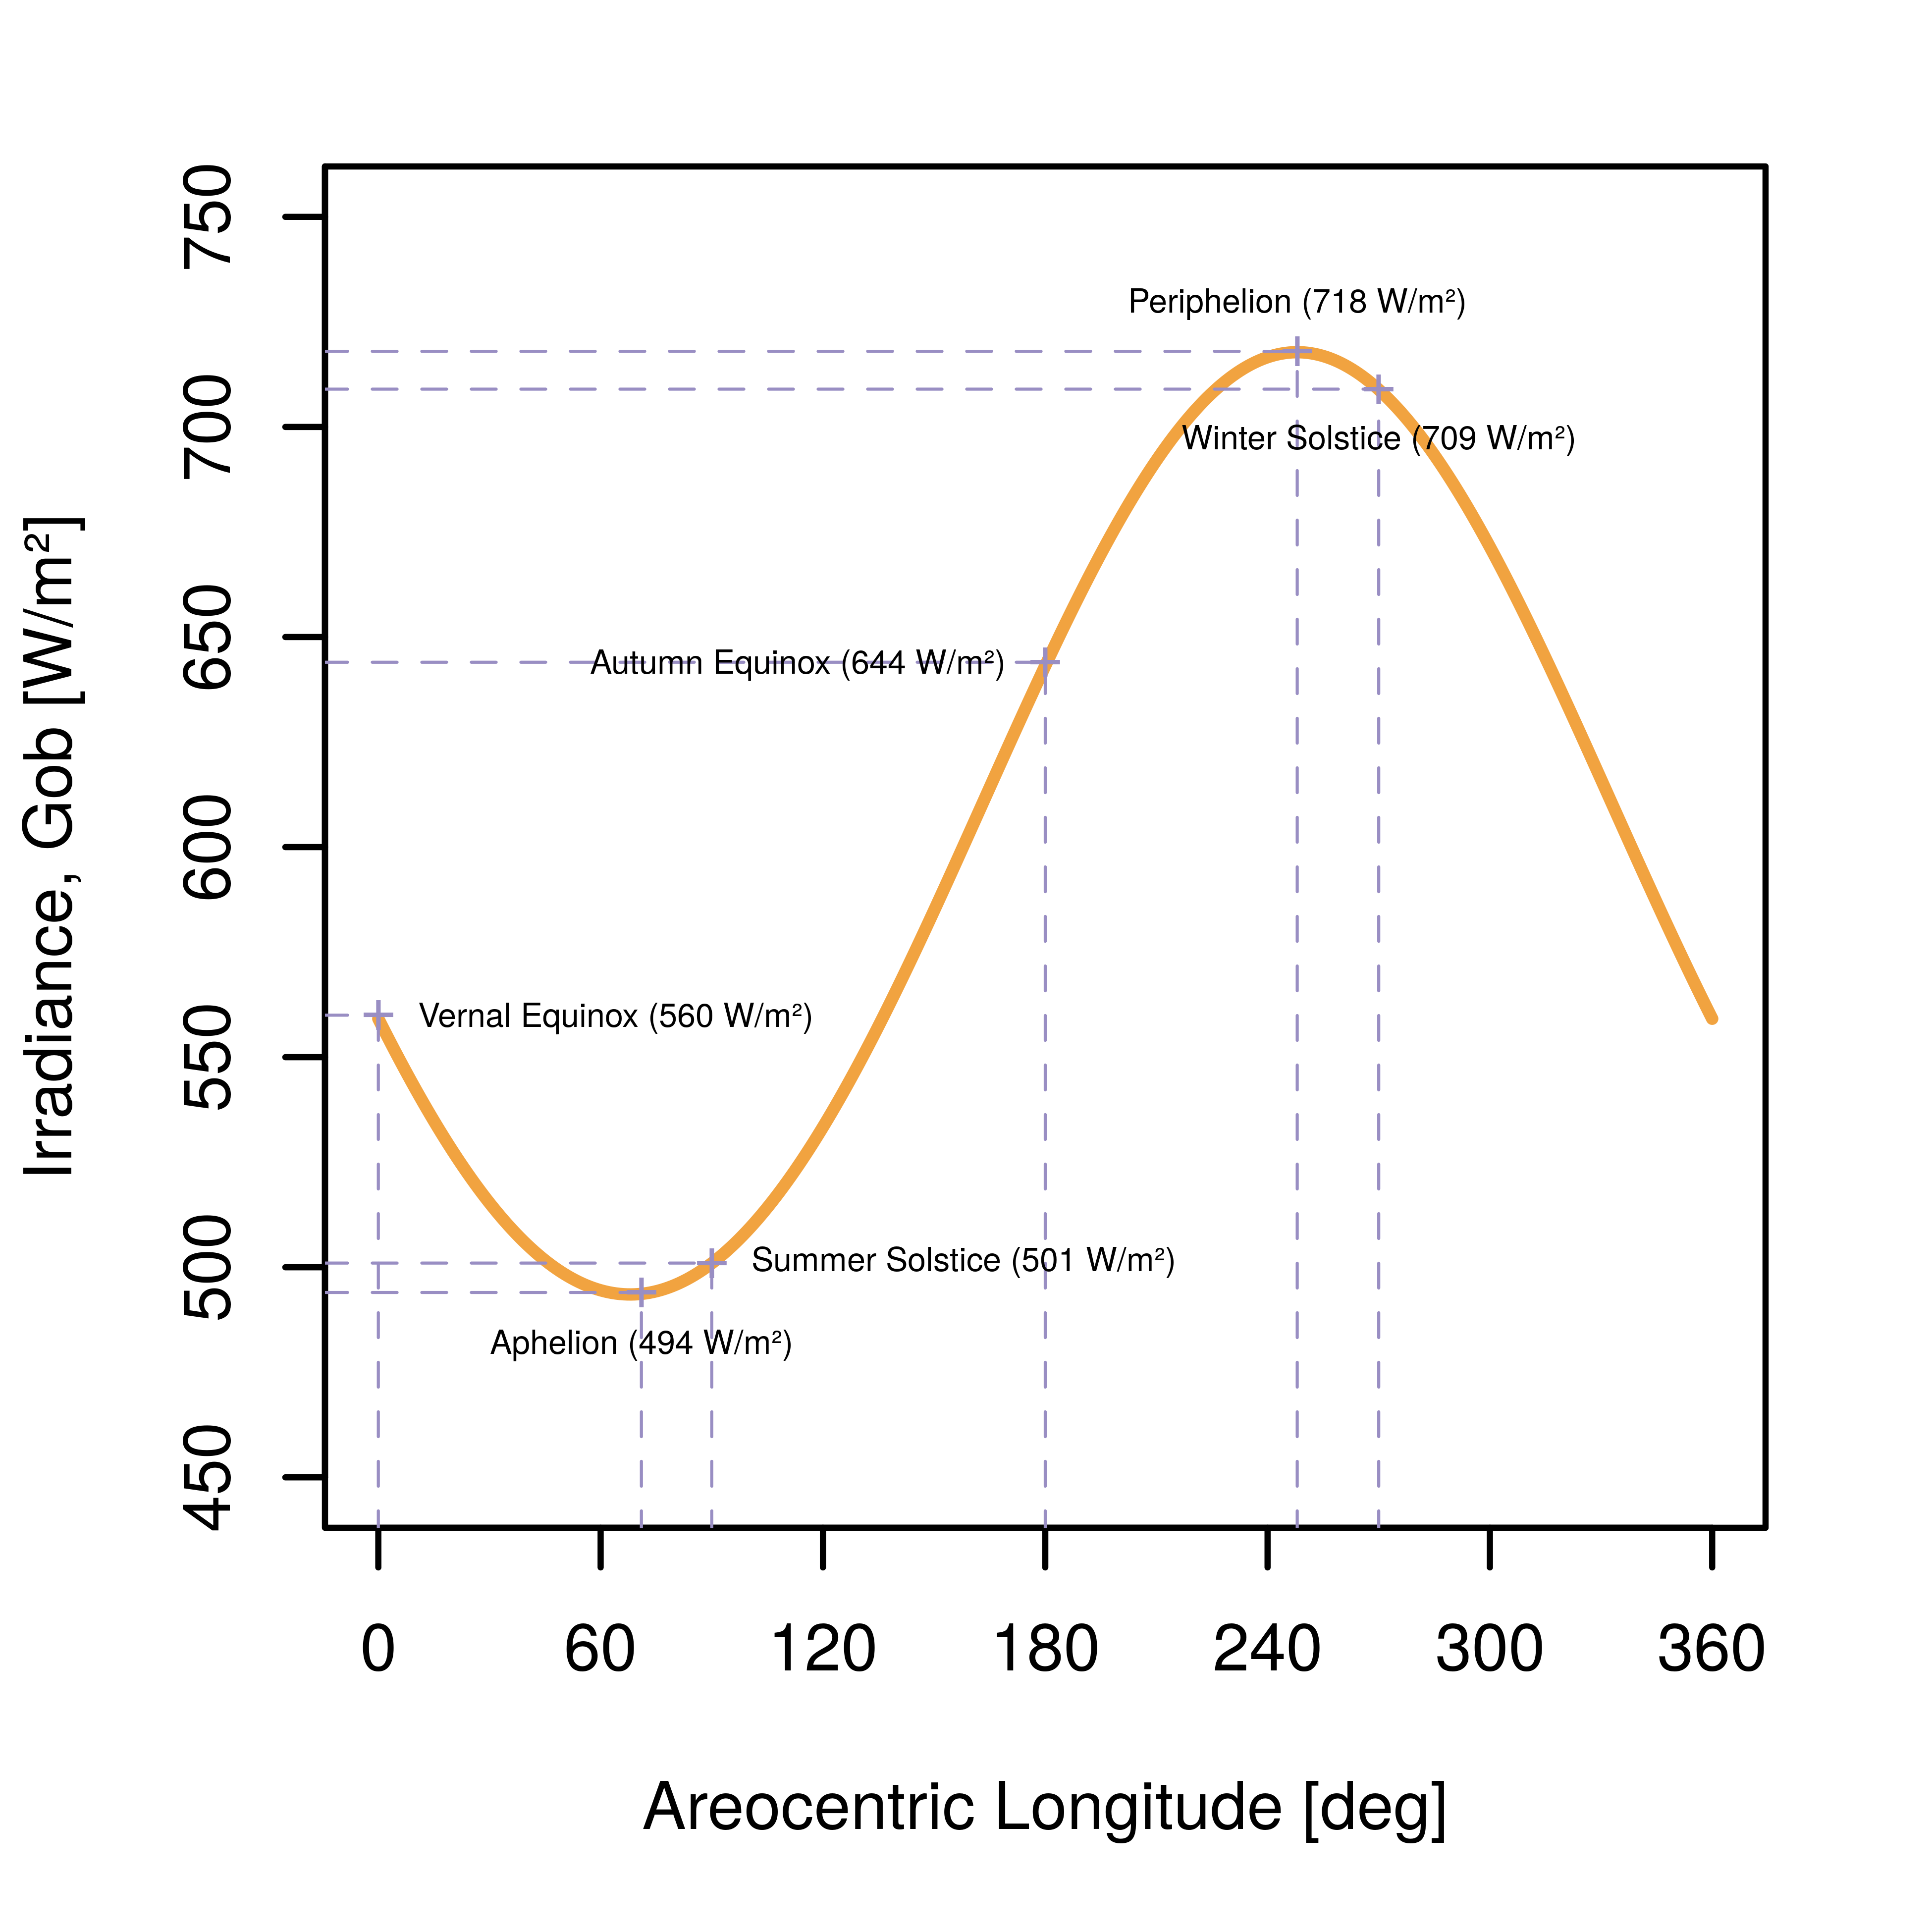
\includegraphics[width=0.8\linewidth]{sections/martian-environment/plots/gob-daily-variations.png}\\
  \caption[Beam irradiance at top of Mars atmosphere as a function of Areocentric Longitude]
          {Beam irradiance at top of Mars atmosphere as a function of Areocentric Longitude}
  \label{fig:plot:beam-irradiance-top-of-mars-atmosphere}
\end{figure}

Further parameterization becomes necessary in order to measure beam irradiance on a horizontal surface at the top Mars atmosphere where the solar zenith angle $z$ must be considered. The solar zenith angle itself is a function of planetary latitude $\phi$, declination angle $\delta$, and hour angle $\omega$ measured from the true noon westward \citemarsenv{Appelbaum1990}. Expressed as $G_{obh}$, it is presented in Equation \ref{eq:G_obh}:

\begin{equation}
  \label{eq:G_obh}
  G_{obh} = G_{ob}\cos{z}
\end{equation}

where $z$ is given by:

\begin{equation}
  \label{eq:cosz}
  \cos{z} = \sin{\phi}\sin{\delta} + \cos{\phi}\cos{\delta}\cos{\omega}
\end{equation}

Solar radiation calculations using Equation \ref{eq:G_obh} as a function of Solar time are presented in Figure \ref{fig:plot:diurnal-variation-of-beam-irradiance-on-a-horizontal-surface-at-top-of-mars-atmosphere}.

\begin{figure}[H]
  \centering
  \hypersetup{linkcolor=captionTextColor}
  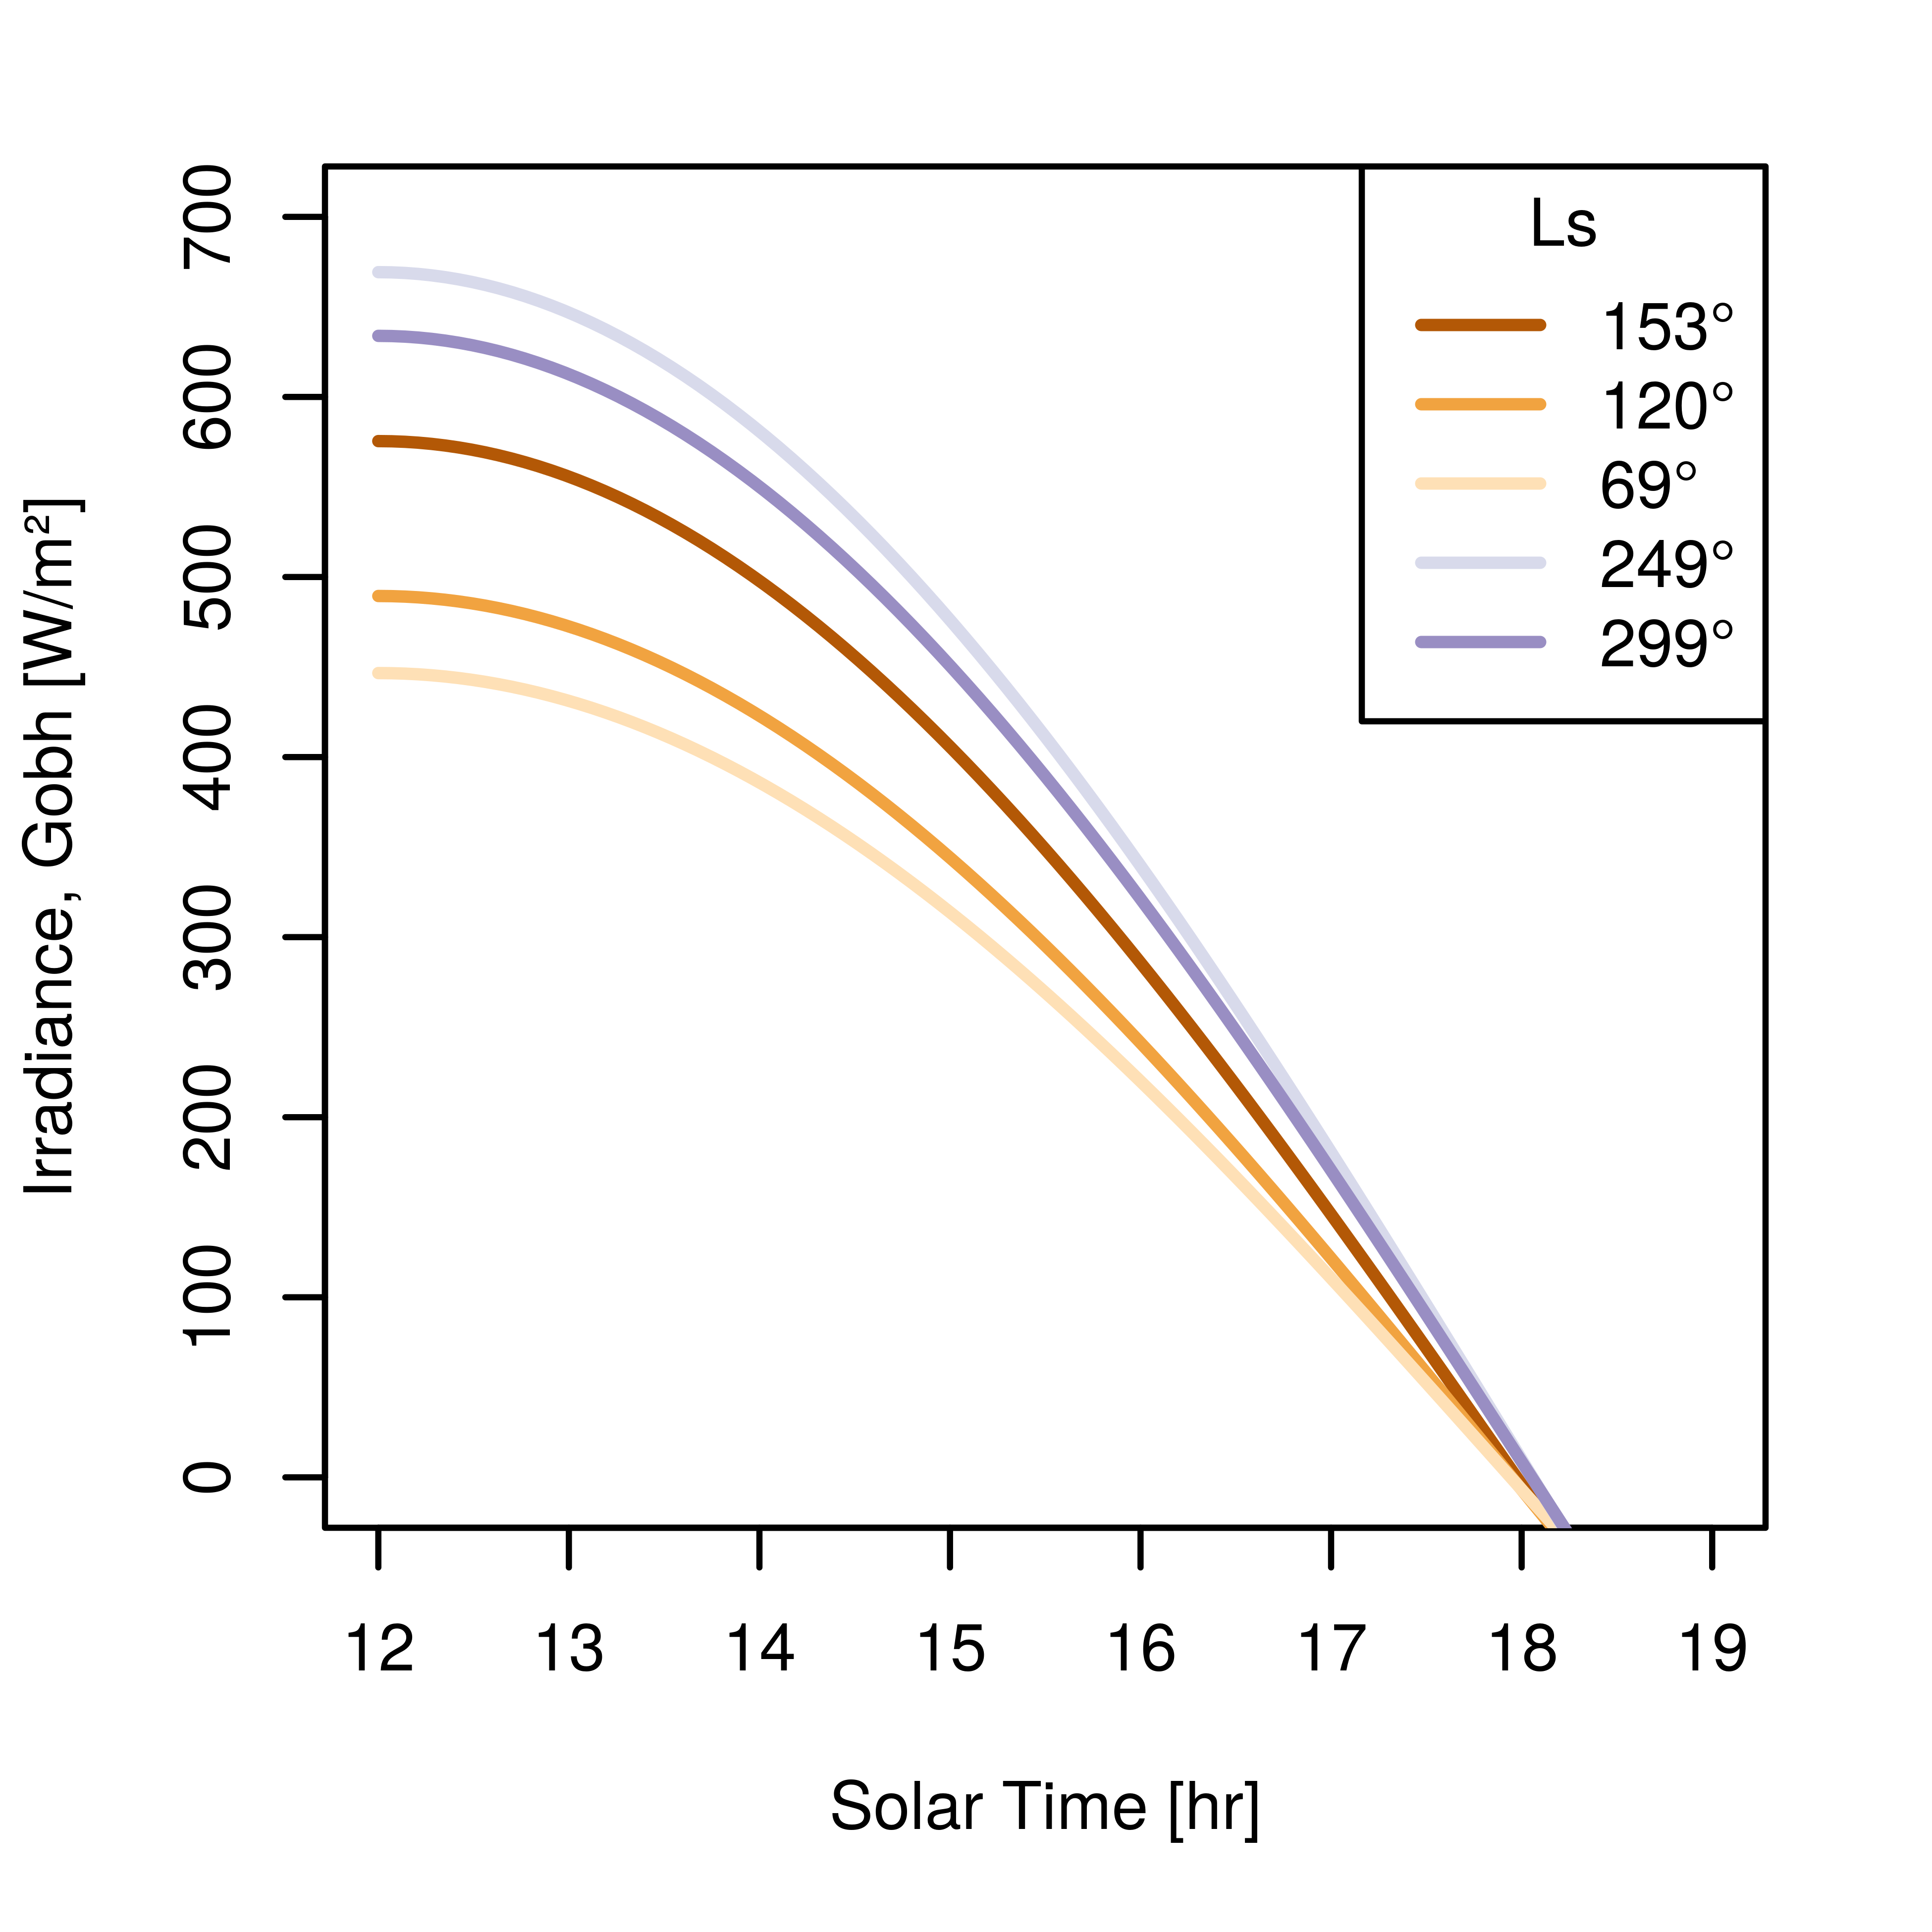
\includegraphics[width=0.8\linewidth]{sections/martian-environment/plots/gobh-diurnal-over-endaveaour-crater.png}\\
  \caption[Diurnal variation of beam irradiance on a horizontal surface at top of Mars atmosphere above Endaveaour Crater]
  {Diurnal variation of beam irradiance on a horizontal surface at top of Mars atmosphere above Endaveaour Crater.}
  \label{fig:plot:diurnal-variation-of-beam-irradiance-on-a-horizontal-surface-at-top-of-mars-atmosphere}
\end{figure}

Obtaining the irradiance on the surface of Mars requires the atmospheric opacity $\tau$ as an additional parameter. A distinction exists between global, direct, and diffuse beam irradiance where global beam irradiance $G_{h}$ is the sum of direct, $G_{bh}$, and diffuse beam irradiances, $G_{dh}$:

\todo[inline]{TODO: Explain scattering a bit or at least mention it.}
% TOOD: Mention scattering: https://ntrs.nasa.gov/archive/nasa/casi.ntrs.nasa.gov/20040191326.pdf

\begin{equation}
  \label{eq:G_h_1}
  G_{h} = G_{bh} + G_{dh}
\end{equation}

The expression for $G_{h}$ and $G_{bh}$ are presented in Equations \ref{eq:G_h} and \ref{eq:G_bh}:

\begin{equation}
  \label{eq:G_h_2}
  G_{h} = G_{ob}\cos{z}\frac{f(z,\tau)}{0.9}
\end{equation}

where $f(z,\tau)$ is the normalized net flux function derived from the net solar flux integrated over the solar spectrum on the Martian surface and 0.9 comes from the $(1-albedo)$ expression for an albedo of 0.1 \citemarsenv{Appelbaum1990}.

\begin{equation}
  \label{eq:G_bh}
  G_{bh} = G_{ob}\cos{z}\exp(\frac{-\tau}{cos{z}})
\end{equation}

Diurnal irradiance profiles at Endaveour Crater are presented in Figure \ref{fig:plot:irradiances-phi} for different planetary latitudes during the perihelion. At $L_{s} = \SI{248}{\degree}$ the northern hemisphere is in mid-Autumn whereas the southern hemisphere in mid-Spring, as such irradiances are much larger at $\phi = \SI{-40}{\degree}$ and $\phi = \SI{-20}{\degree}$ than they are at $\phi = \SI{0}{\degree}$ and $\phi = \SI{40}{\degree}$.

\begin{figure}[H]
\captionsetup[subfigure]{justification=centering}
\vspace{-2ex}
	\centering
    %% setup sizes
    \setlength{\subfigureWidth}{0.50\textwidth}
    \setlength{\graphicsHeight}{80mm}
    %% kill hyper-link highlighting
    \hypersetup{hidelinks=true}%
    %% the figures
%% 1st row
  	\begin{subfigure}[t]{\subfigureWidth}
      \centering
  		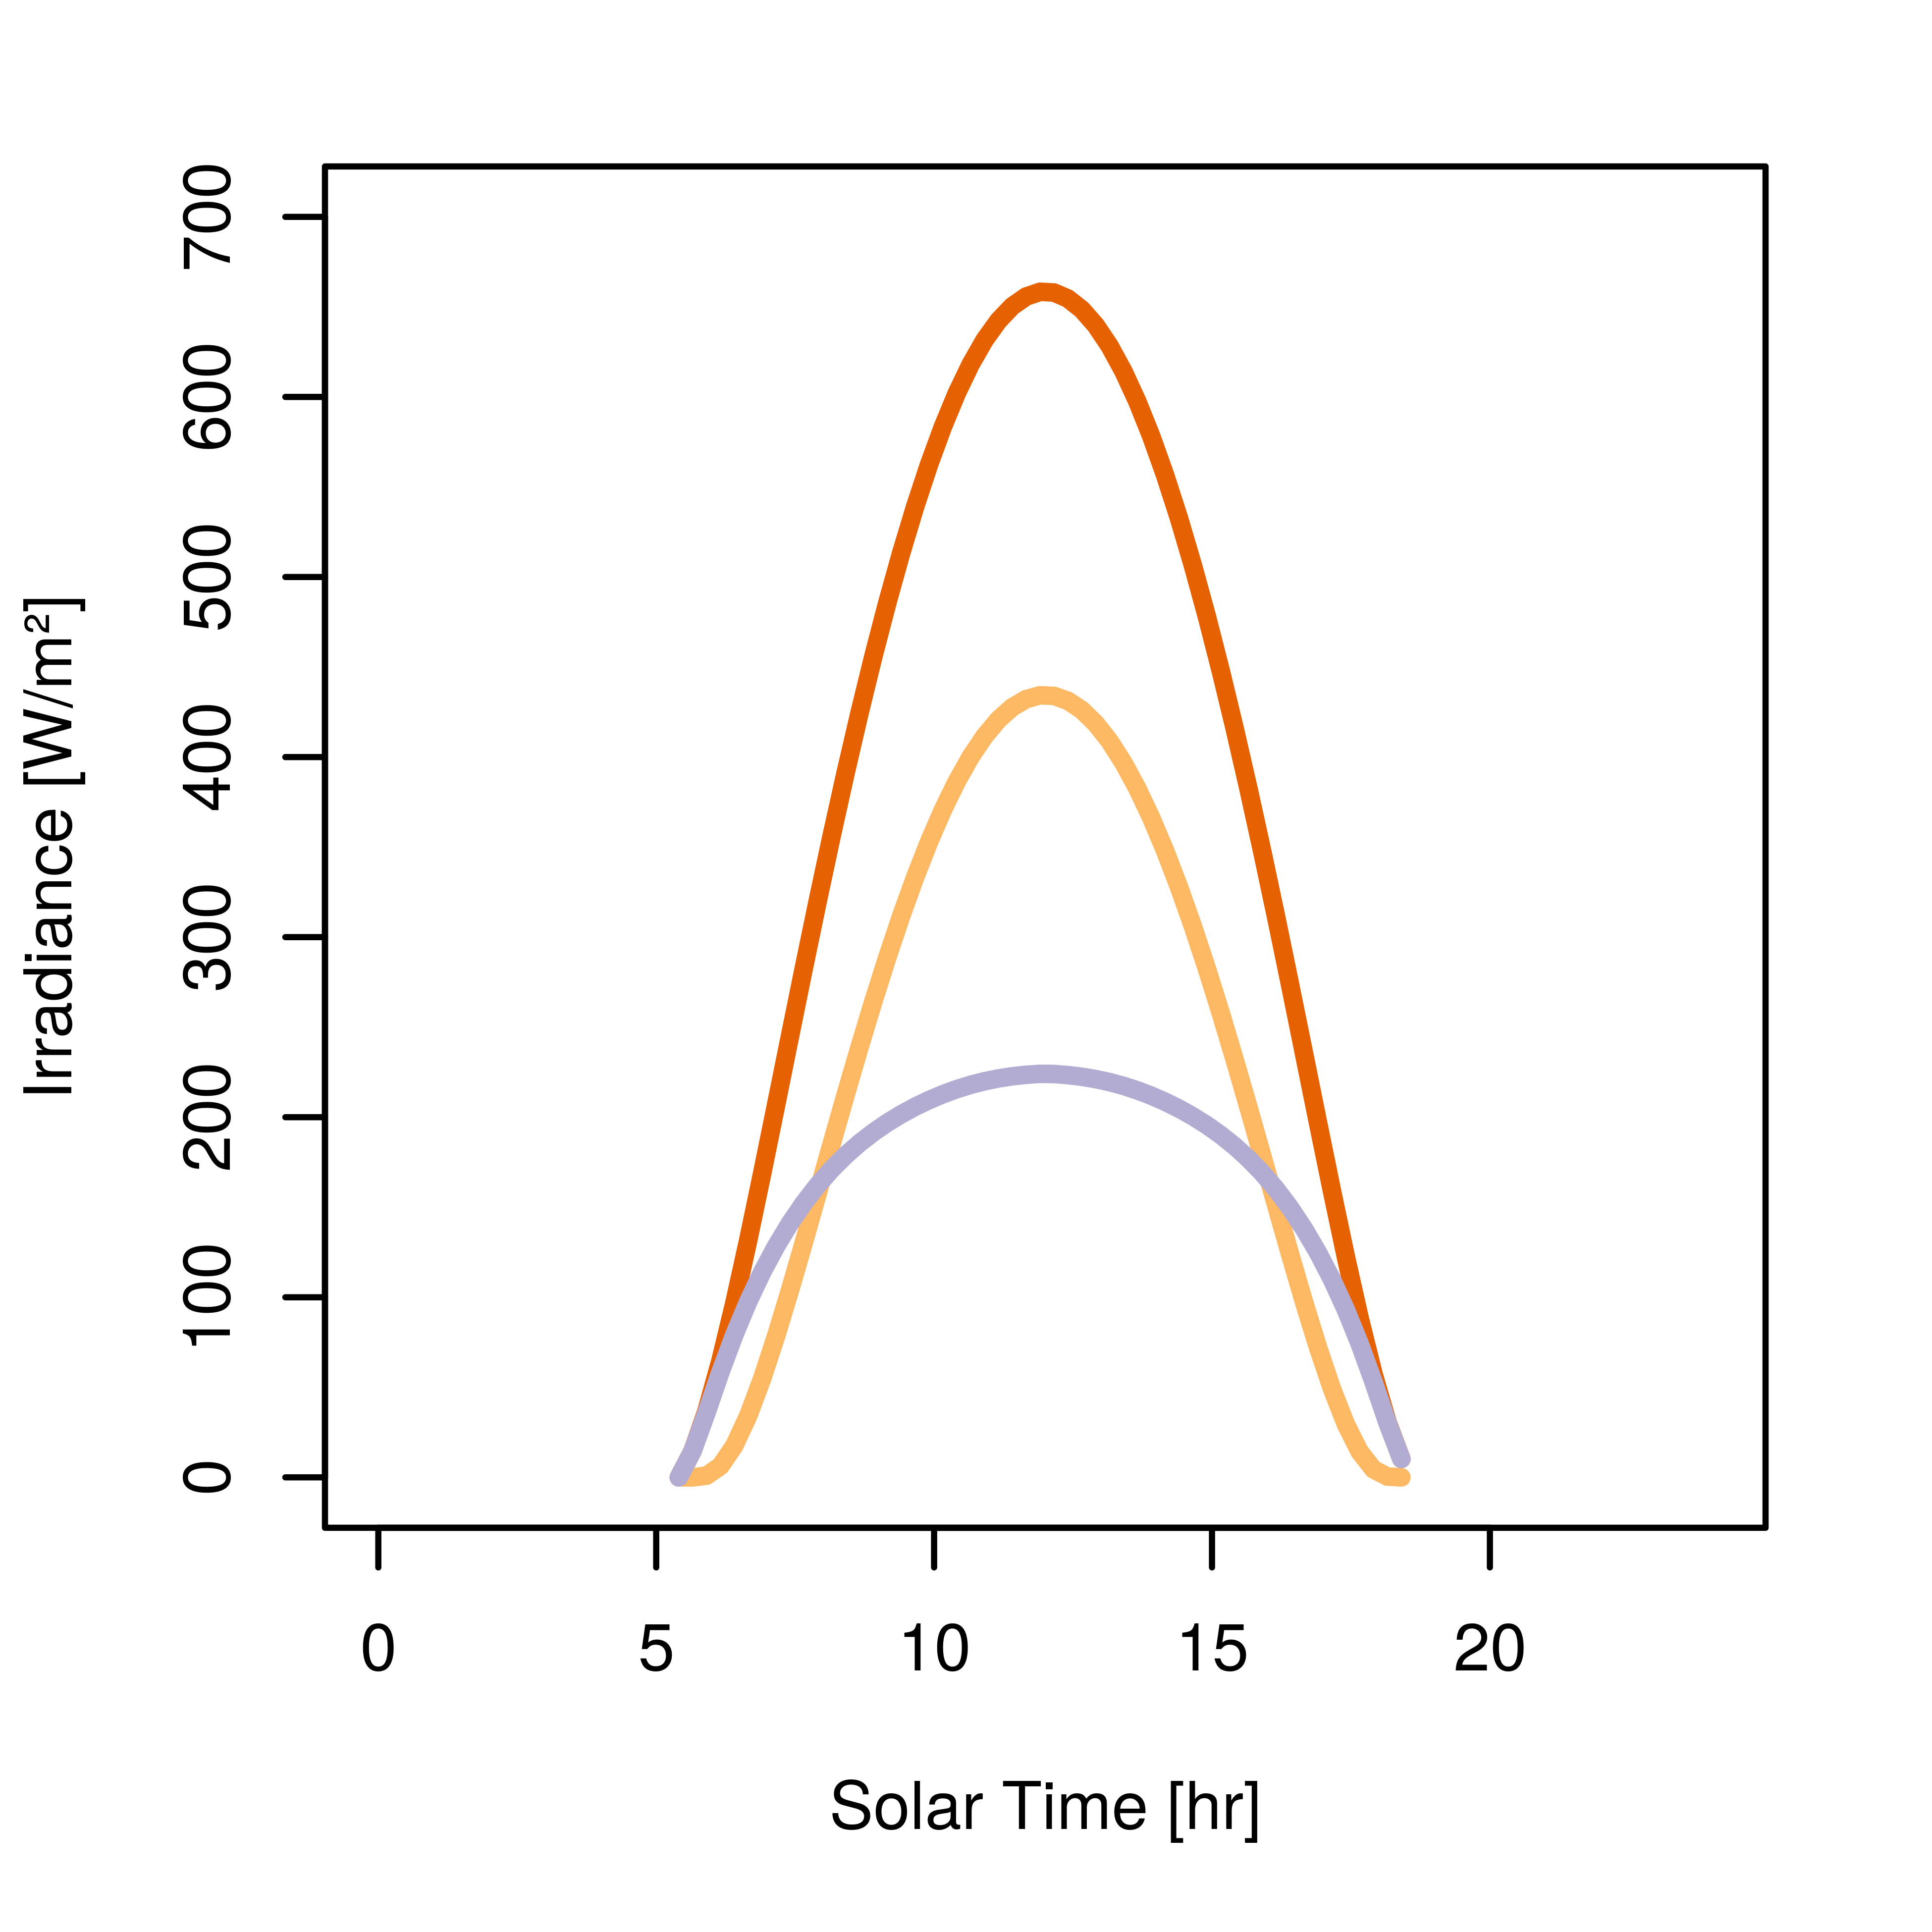
\includegraphics[height=\graphicsHeight]{sections/martian-environment/plots/gh-gbh-gdh-variation-1-for-ls-248-phi-20-tau-05-and-albedo-027.png}
  		\subcaption{$\phi = \SI{-40}{\degree}$}
  		\label{fig:sub:irradiance-phi-m20}
  	\end{subfigure}\hfill
    \begin{subfigure}[t]{\subfigureWidth}
      \centering
  		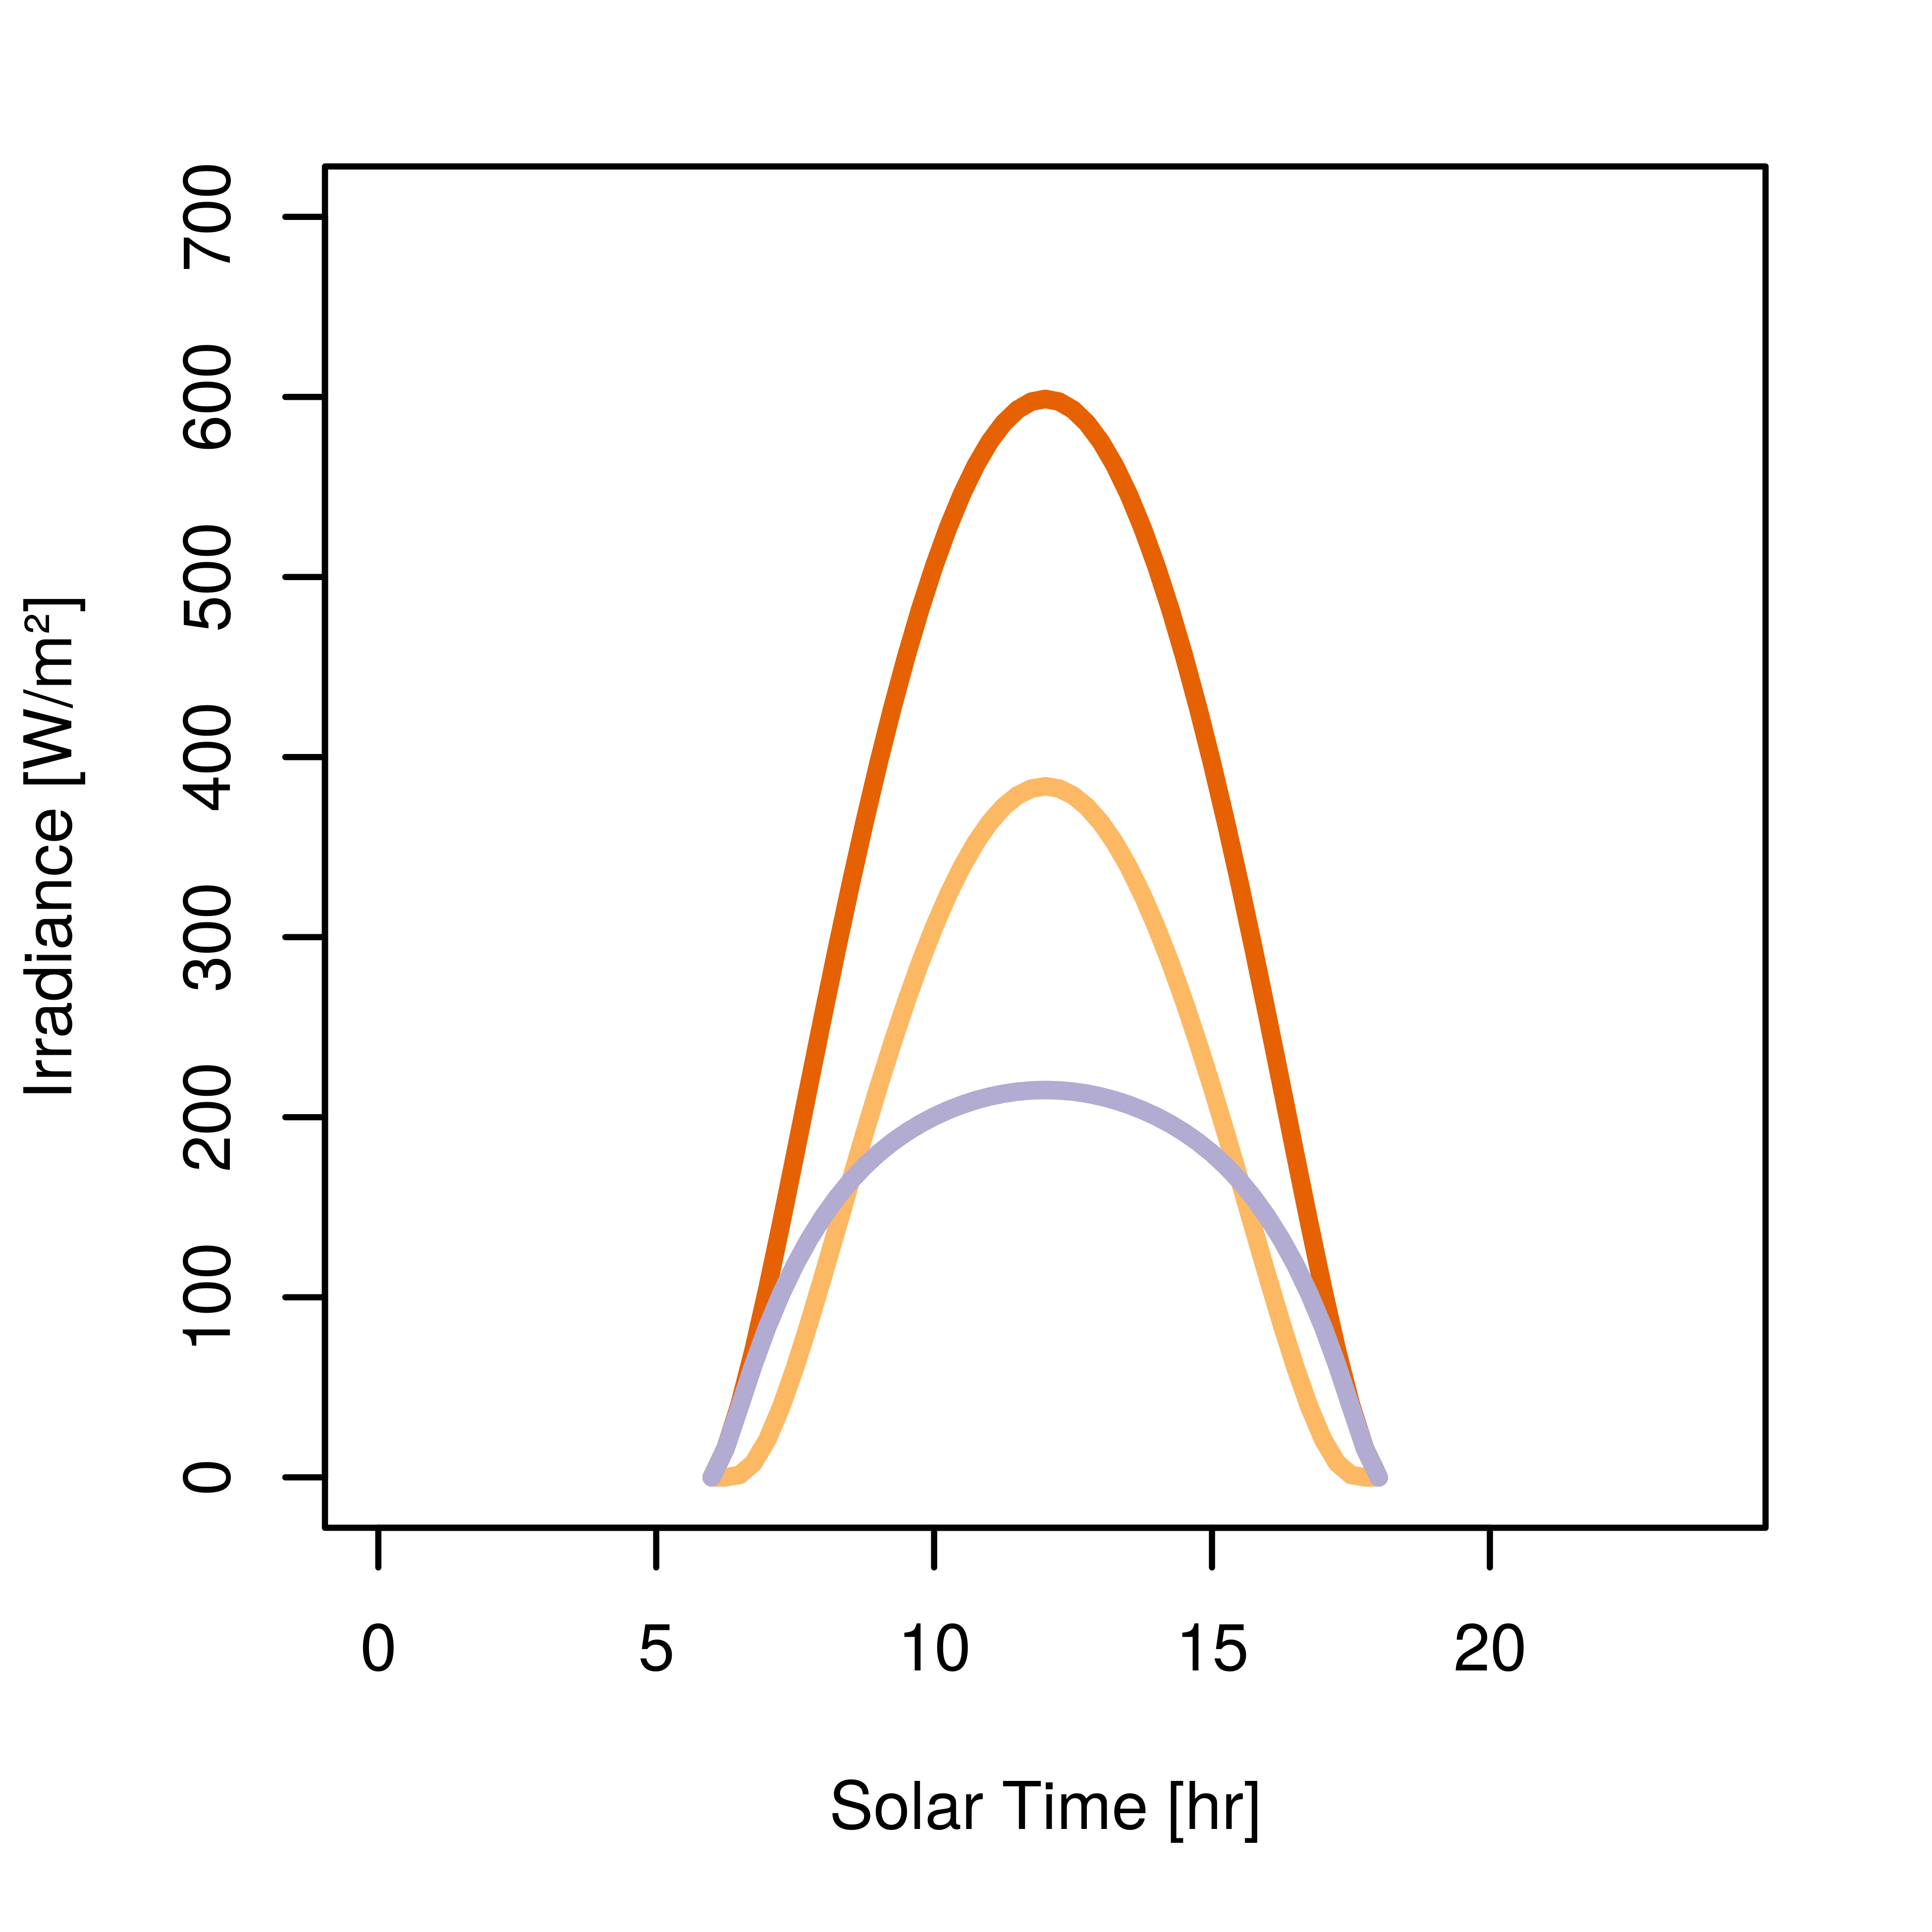
\includegraphics[height=\graphicsHeight]{sections/martian-environment/plots/gh-gbh-gdh-variation-2-for-ls-248-phi-0-tau-05-and-albedo-027.png}
  		\subcaption{$\phi = \SI{-20}{\degree}$}
  		\label{fig:sub:irradiance-phi-0}
  	\end{subfigure}\\[0.8ex]
%% 2nd row
    \begin{subfigure}[t]{\subfigureWidth}
      \centering
  		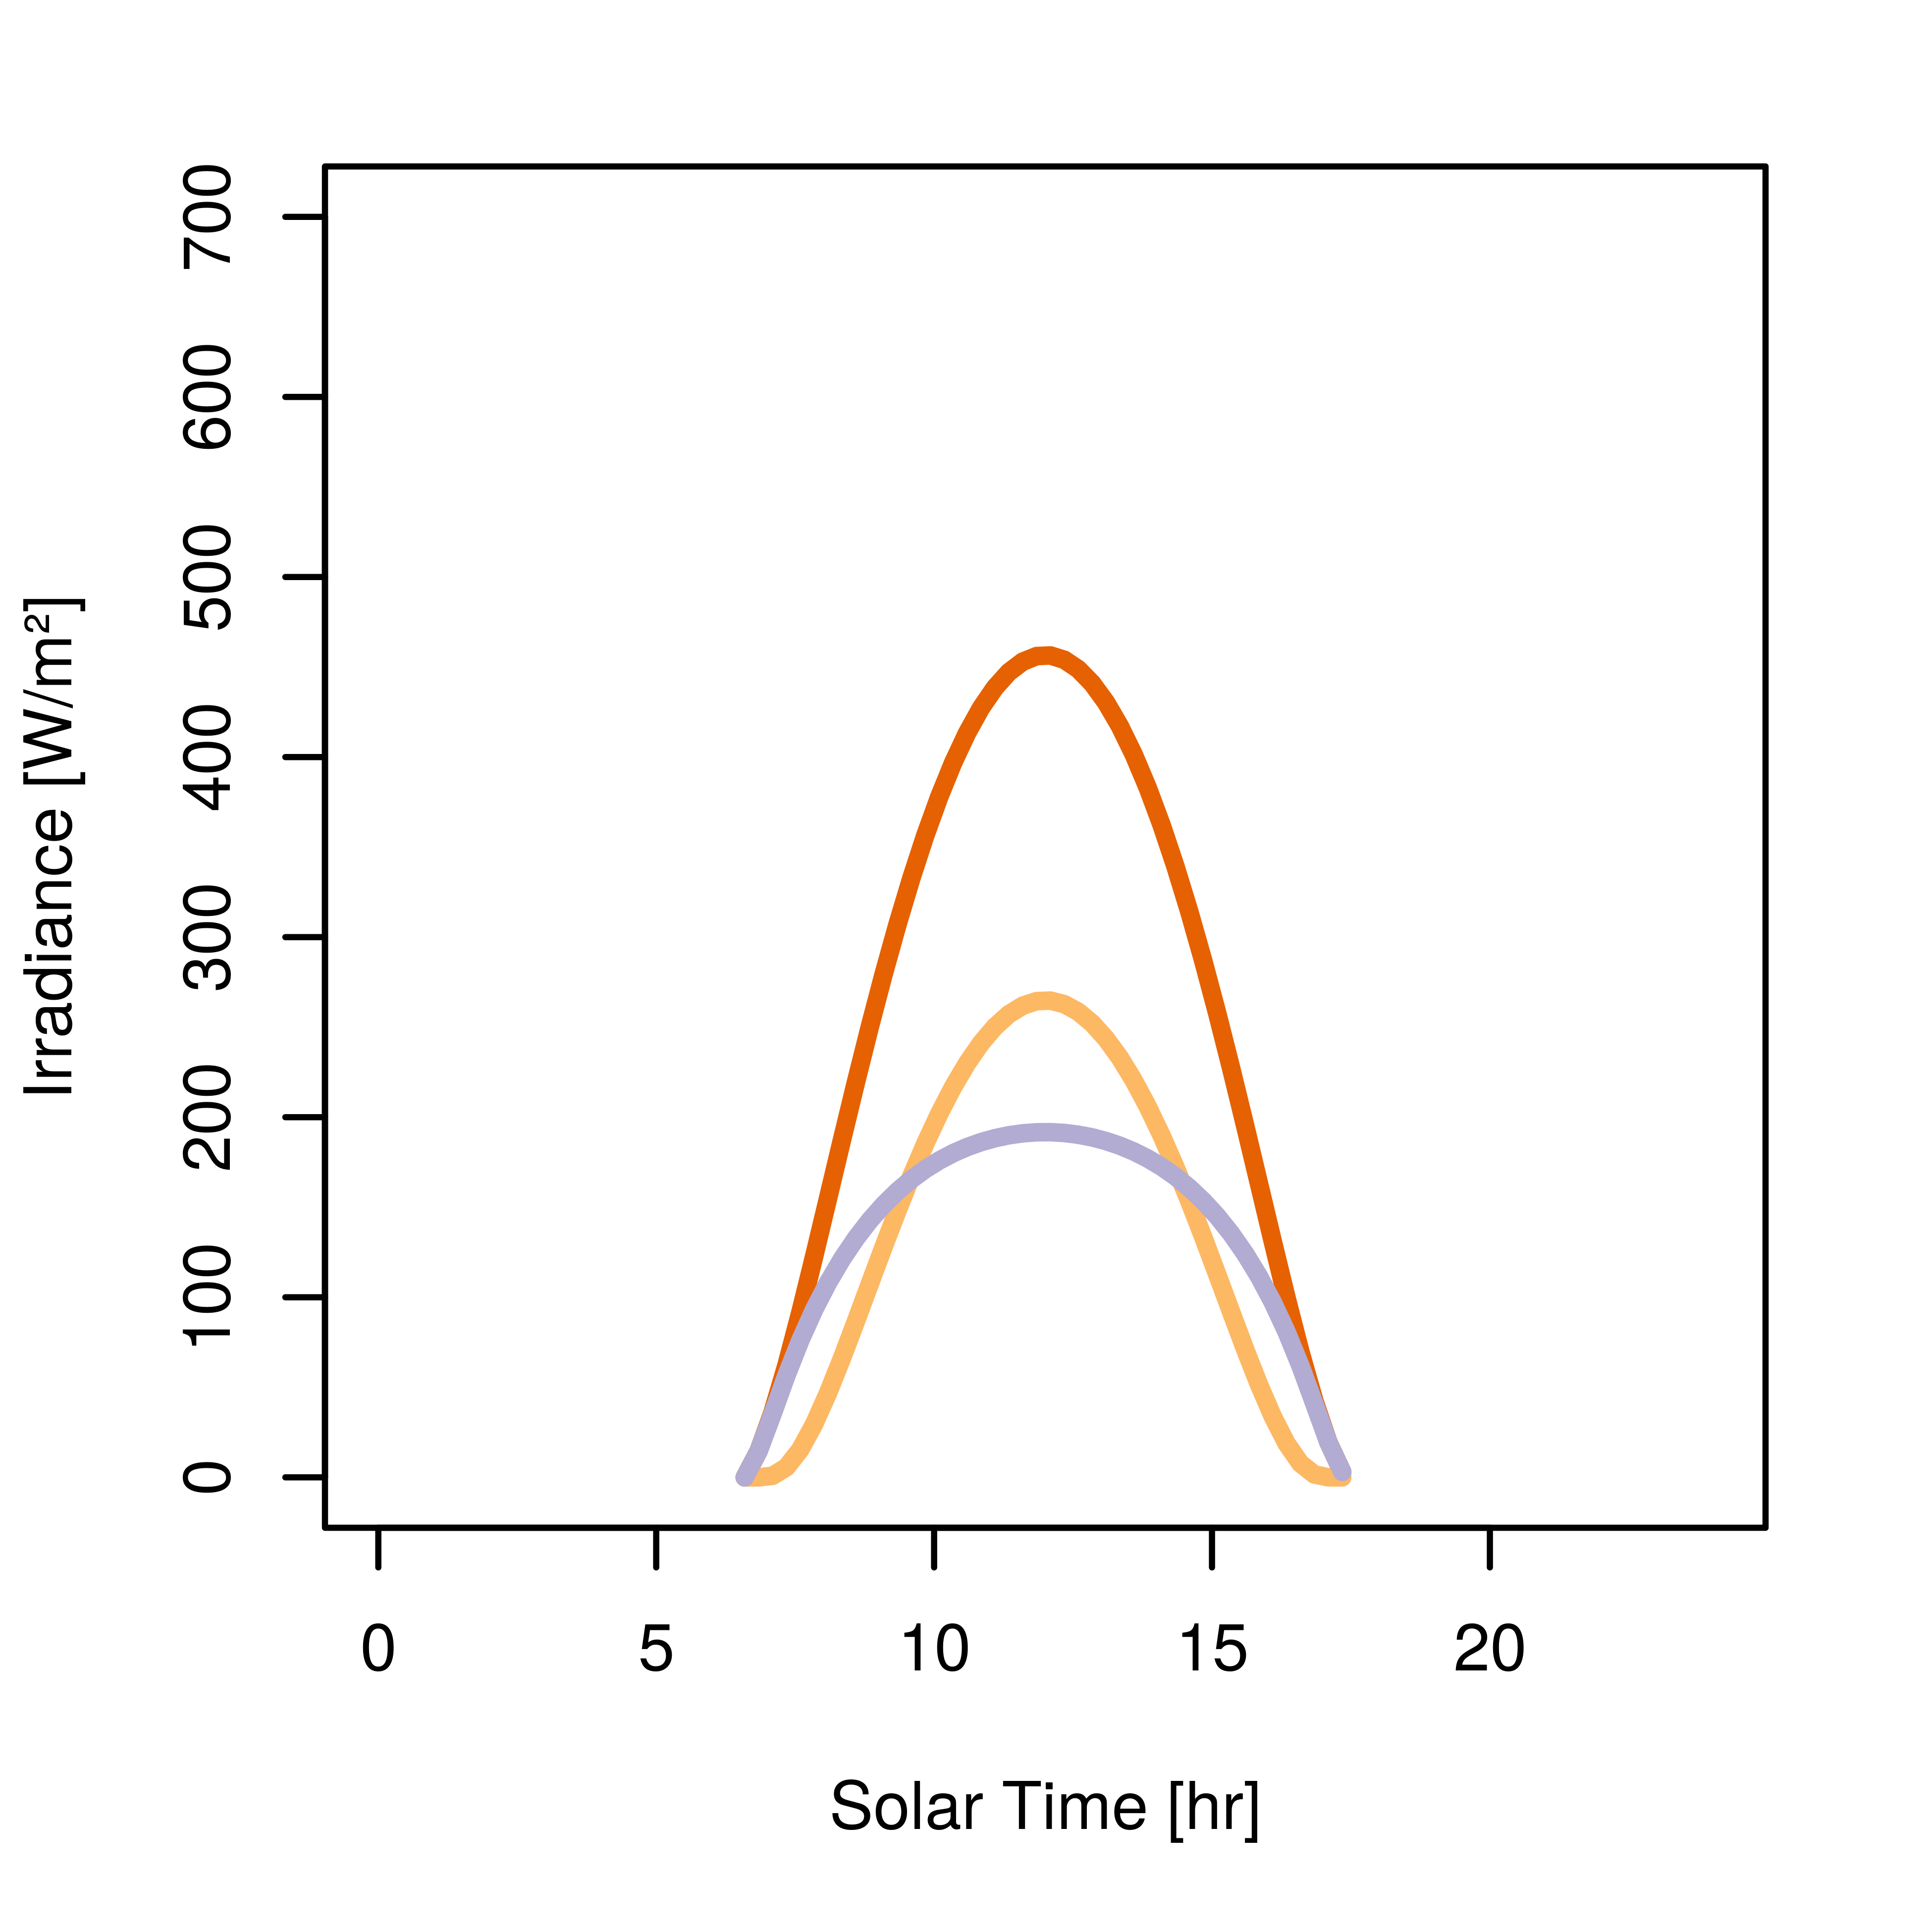
\includegraphics[height=\graphicsHeight]{sections/martian-environment/plots/gh-gbh-gdh-variation-3-for-ls-248-phi-20-tau-05-and-albedo-027.png}
  		\subcaption{$\phi = \SI{0}{\degree}$}
  		\label{fig:sub:irradiance-phi-p20}
  	\end{subfigure}\hfill
	   \begin{subfigure}[t]{\subfigureWidth}
      \centering
  		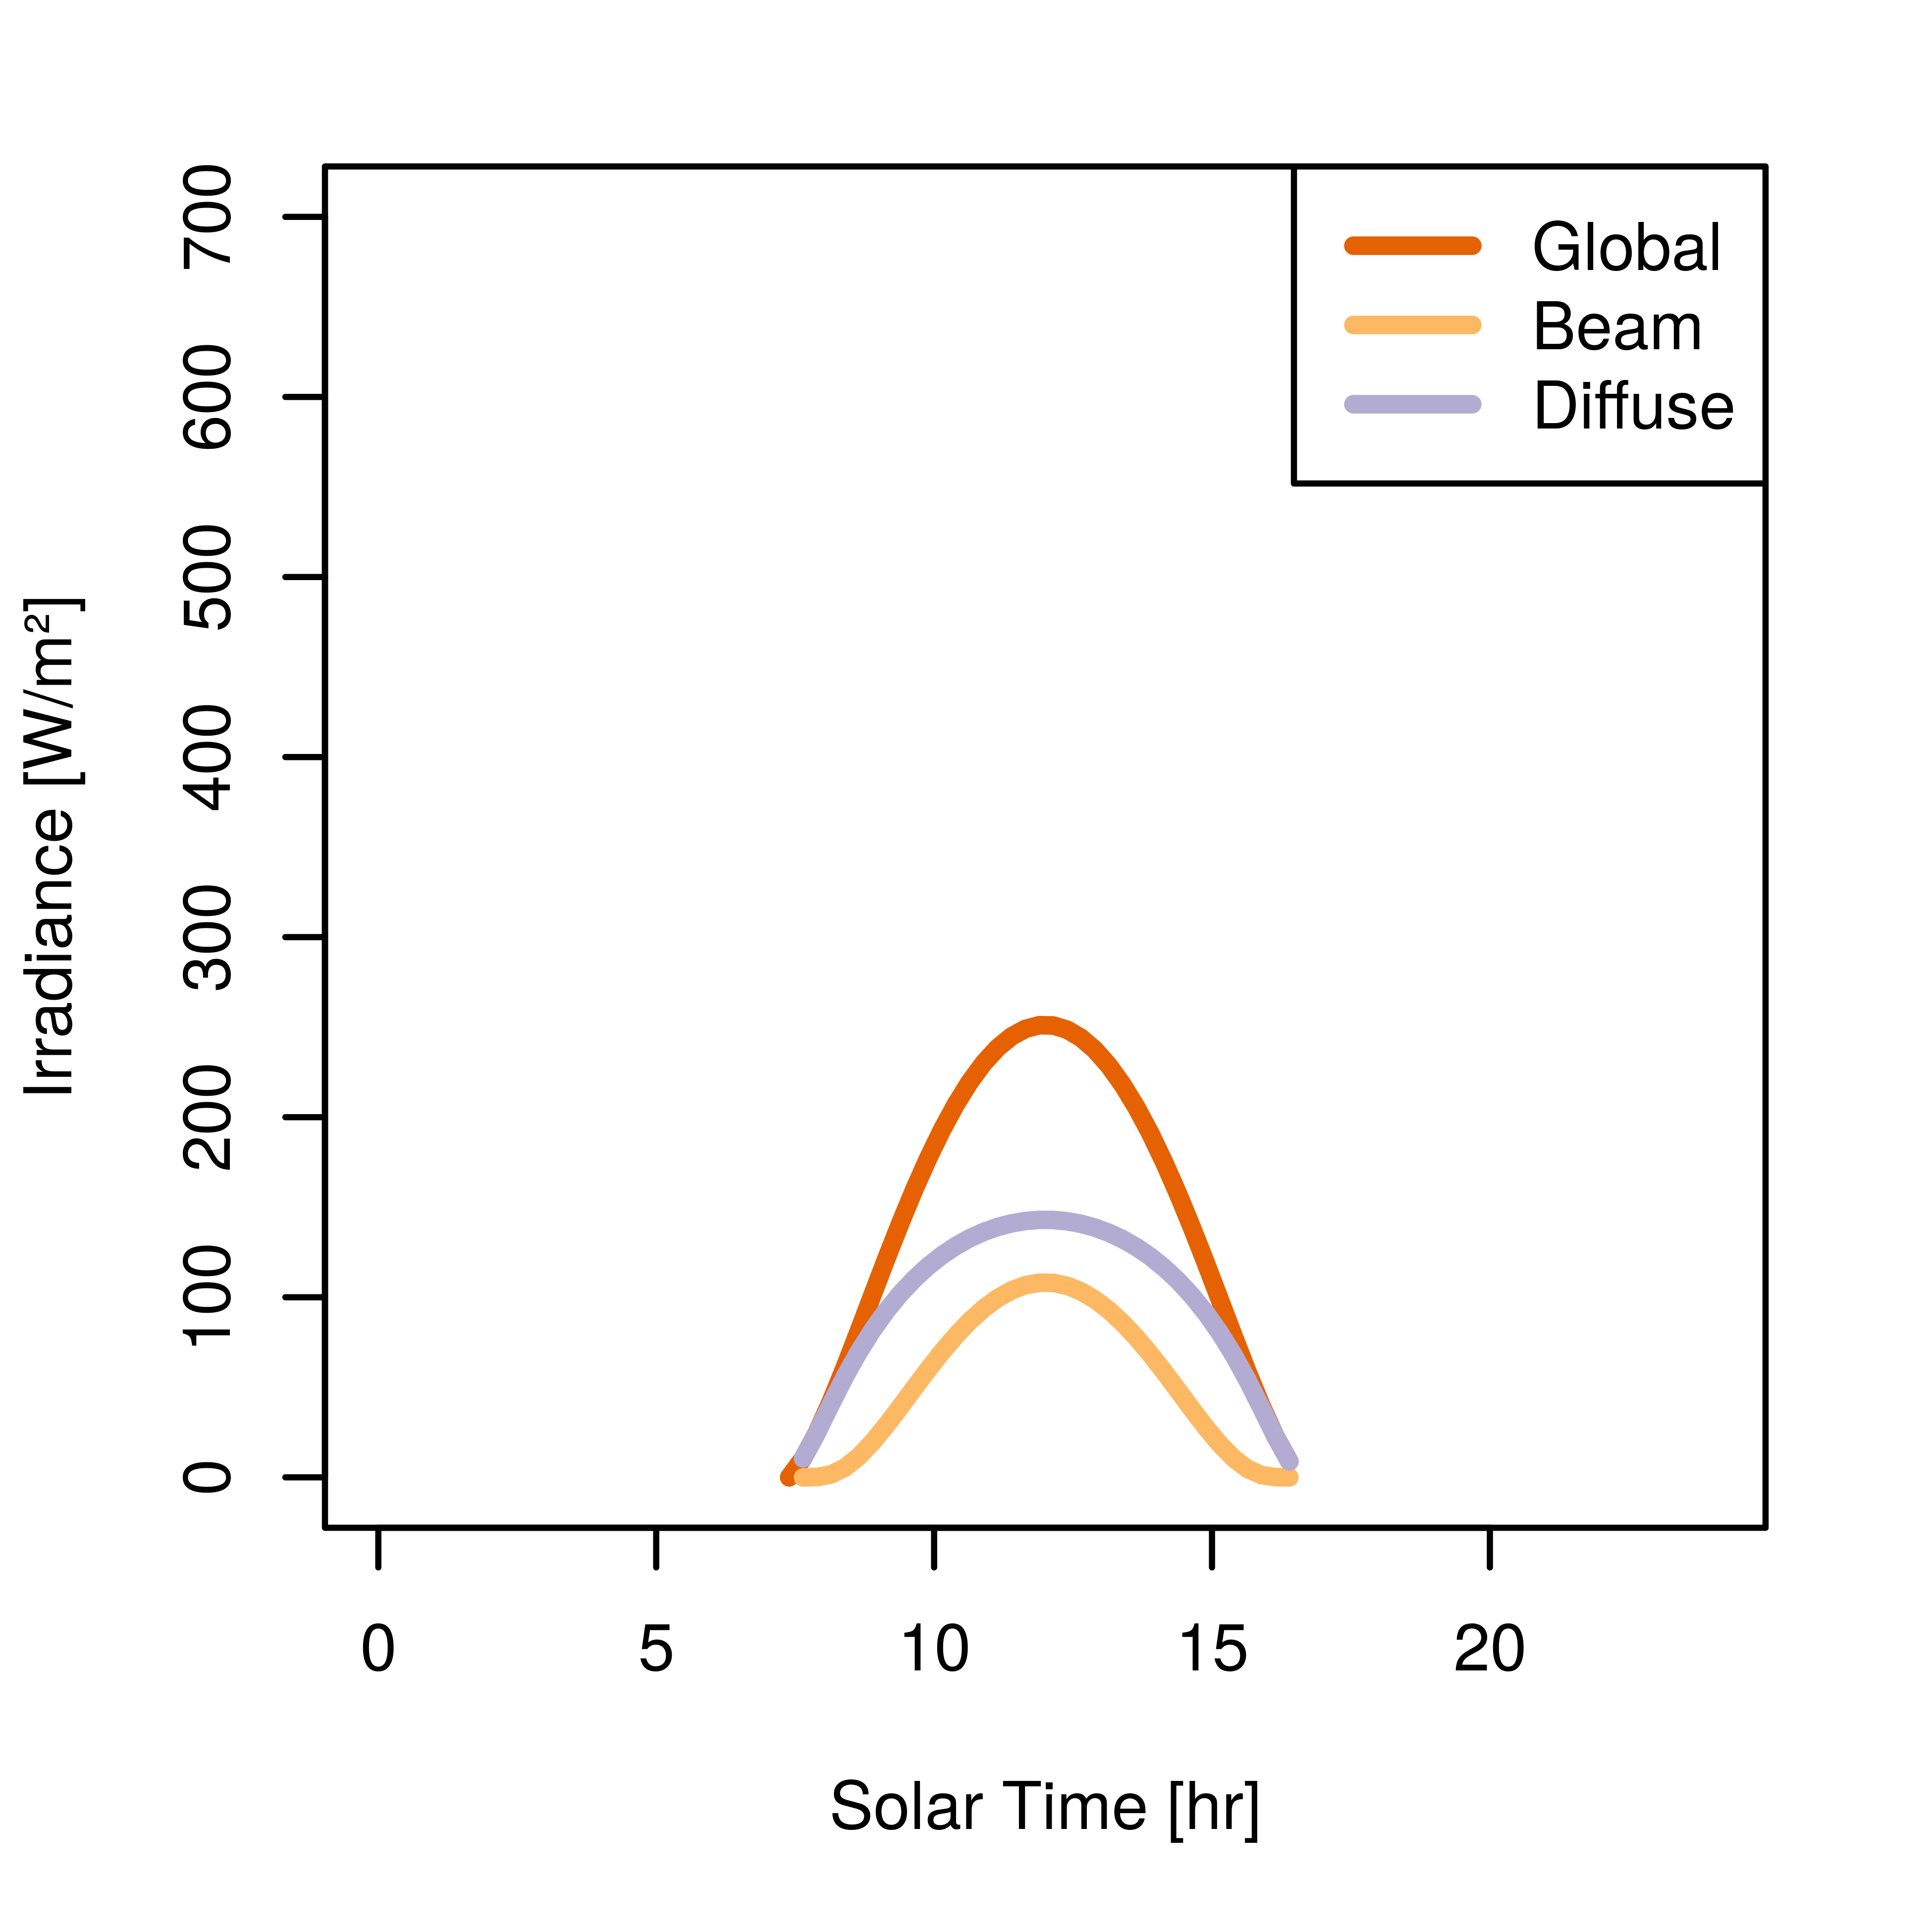
\includegraphics[height=\graphicsHeight]{sections/martian-environment/plots/gh-gbh-gdh-variation-4-for-ls-248-phi-40-tau-05-and-albedo-027.png}
  		\subcaption{$\phi = \SI{20}{\degree}$}
  		\label{fig:sub:irradiance-phi-p40}
	   \end{subfigure}\hfill
	\caption{Diurnal variation of global, beam, and diffuse irradiance on Mars horizontal surface at different planetary latitudes.}
	\label{fig:plot:irradiances-phi}
\vspace{-2ex}
\end{figure}


\subsection{Insolation}
\label{sec:MartianEnvironment:SolarRadiation:Insolation}

Solar insolation is the amount solar radiation incident on a planetary surface during a time period. It is expressed in \si{\watt\hour\per\meter\squared} and obtained by integrating the equations of irradiance over a time period between $\omega_1$ and $\omega_2$. Thus, insolation on a horizontal surface at the top of Mars atmosphere, denoted as $I_{obh}$, is obtained by integrating Equation \ref{eq:G_h_2} of $G_{obh}$.

Global, beam, and diffuse insolations on a horizontal Mars surface are denoted as $I_{h}$, $I_{bh}$, and $I_{dh}$ respectively. Their values are obtained by integrating \ref{eq:G_h_2} for $I_{h}$ and \ref{eq:G_bh} for $I_{bh}$. Diffuse insolation $I_{dh}$ is obtained through the same relationship presented in Equation \ref{eq:G_h_1}. The variation of insolation as a function of $L_{s}$ for different levels of atmospheric opacities are illustrated in Figure \ref{fig:plot:insolation-ls}. Evidently, the insolation curves peak at the perihelion with $L_{s} = \SI{248}{\degree}$ and reach their lowest during the aphelion with $L_{s} = \SI{71}{\degree}$. Interestingly, diffuse insolation is already the largest component contributing to the global insolation at $\tau = 1$ and, on a dusty day at $\tau = 3$, global insolation is mostly diffuse.

\begin{figure}[H]
\captionsetup[subfigure]{justification=centering}
\vspace{-2ex}
	\centering
    %% setup sizes
    \setlength{\subfigureWidth}{0.50\textwidth}
    \setlength{\graphicsHeight}{80mm}
    %% kill hyper-link highlighting
    \hypersetup{hidelinks=true}%
    %% the figures
%% 1st row
  	\begin{subfigure}[t]{\subfigureWidth}
      \centering
  		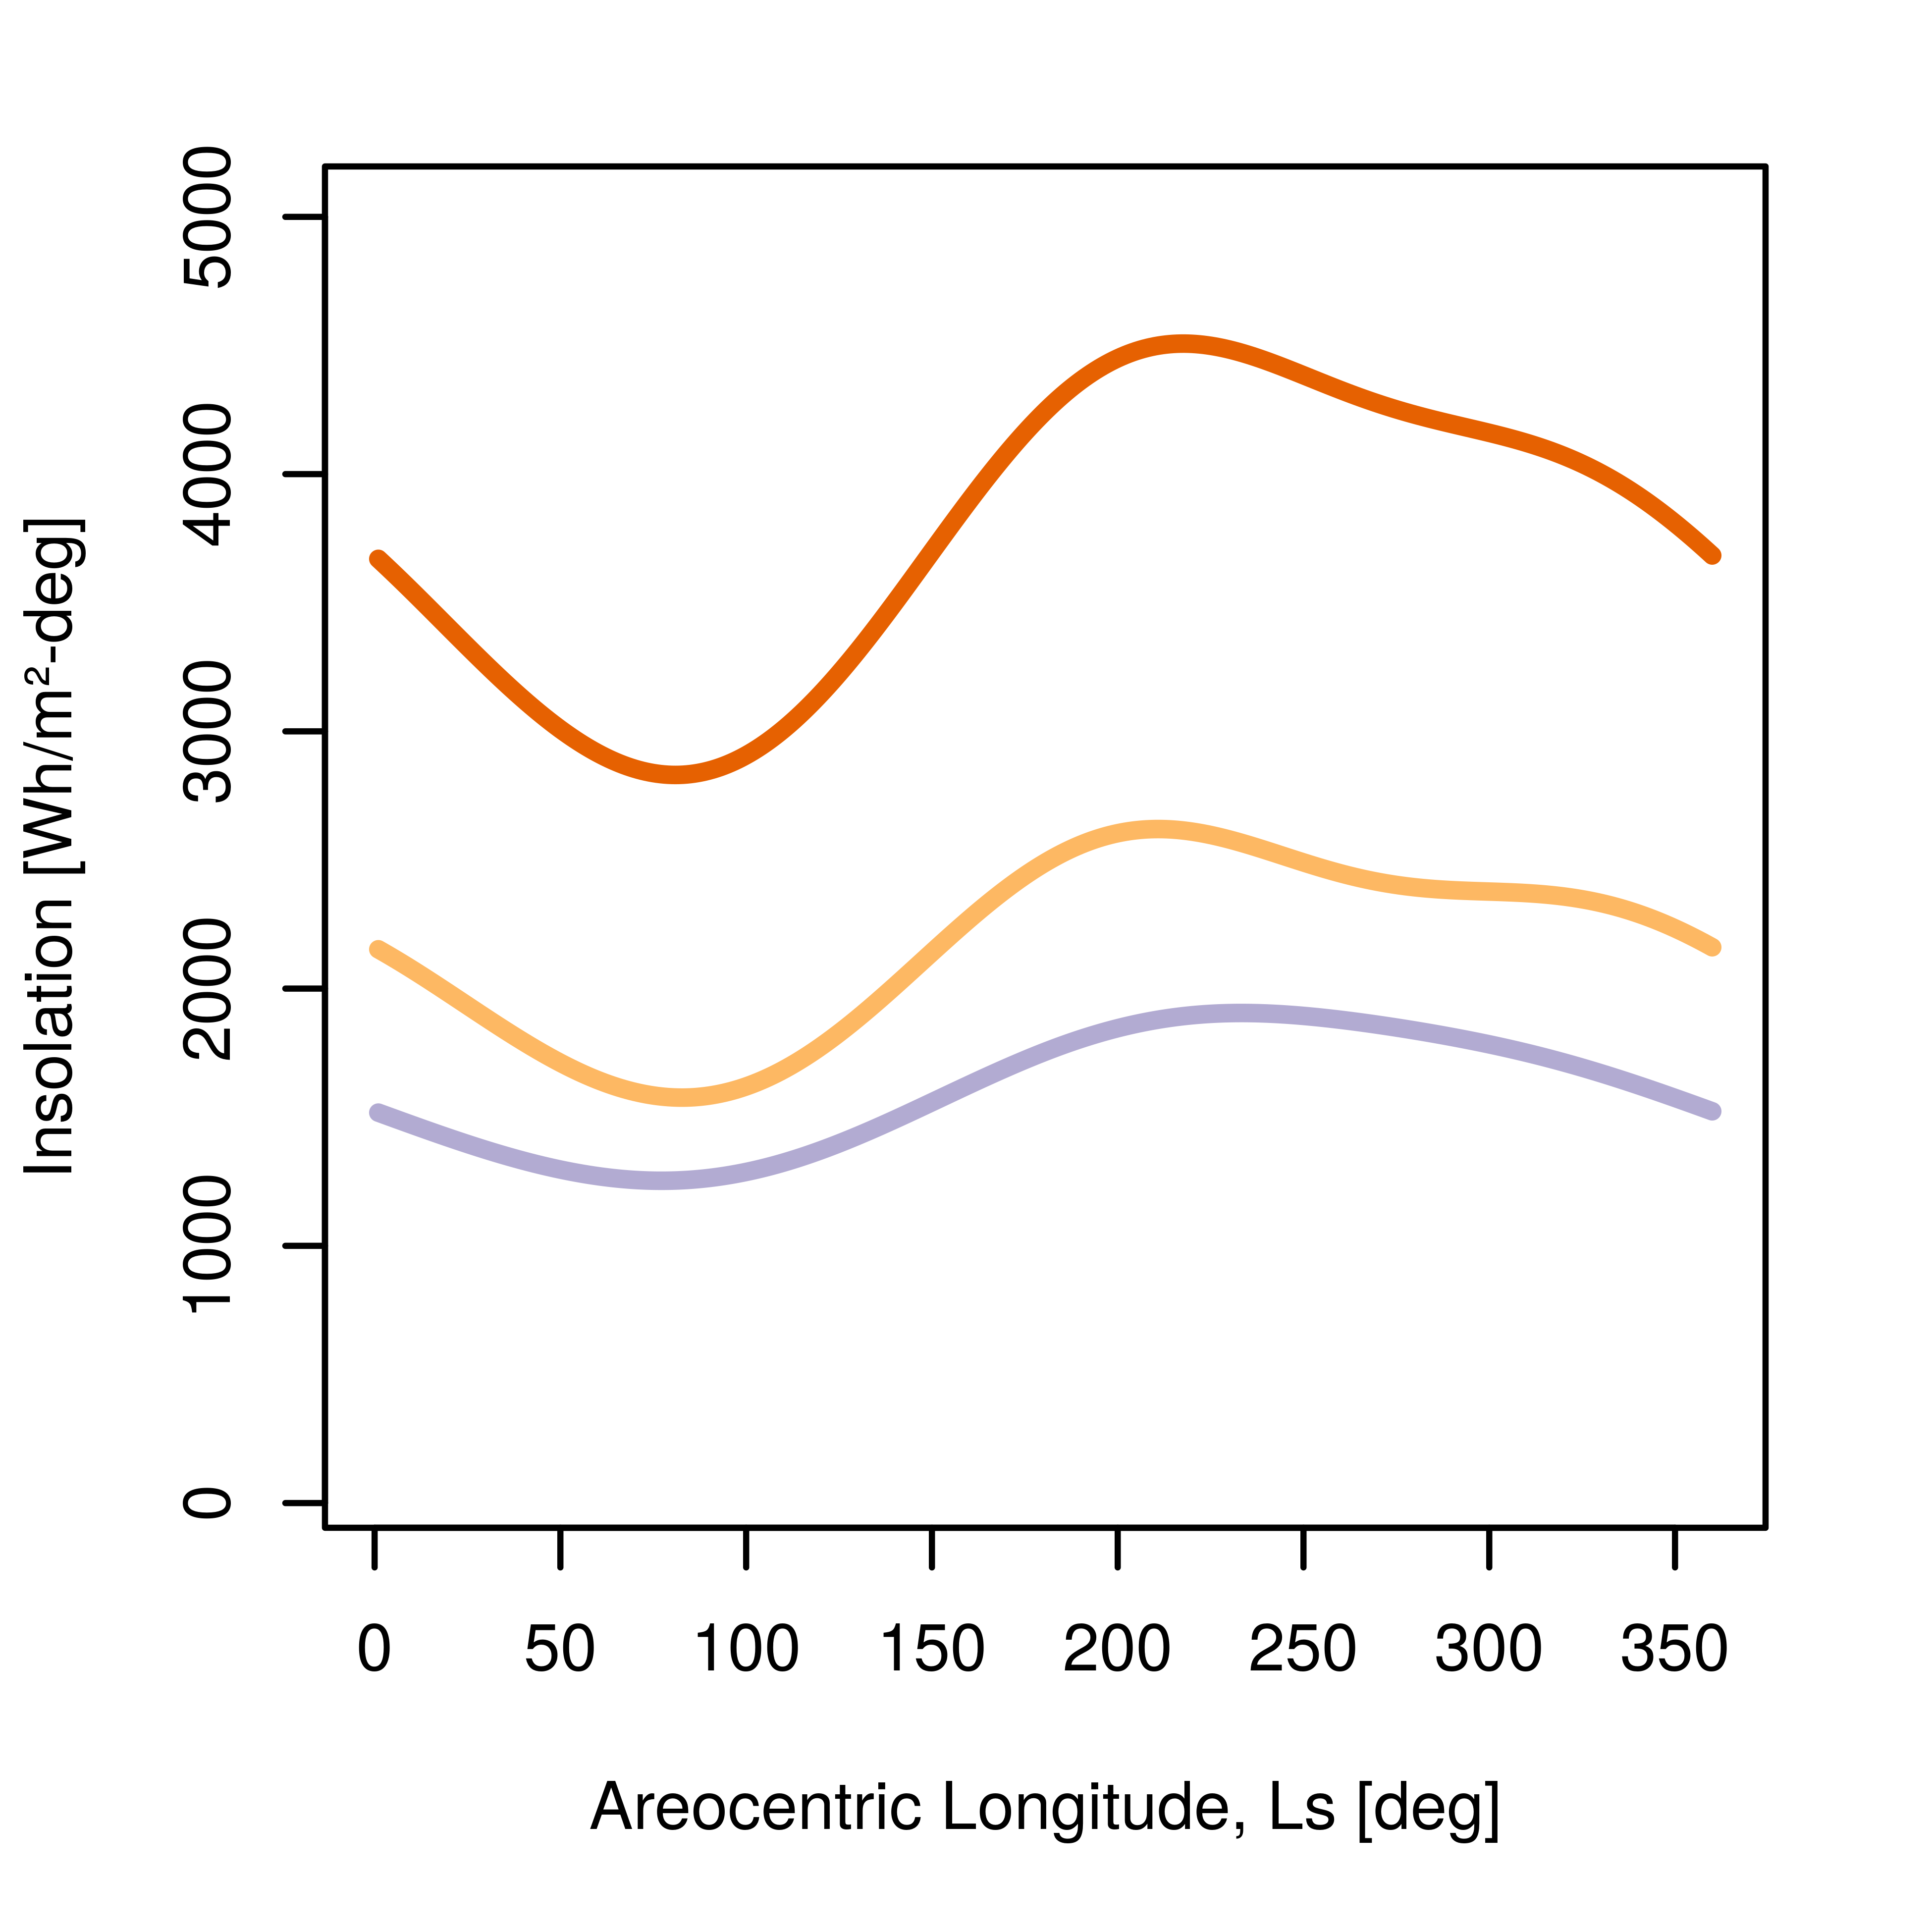
\includegraphics[height=\graphicsHeight]{sections/martian-environment/plots/hh-hbh-and-hdh-as-a-function-of-ls-for-tau05-phi205-and-albedo-027}
  		\subcaption{$\tau = 0.5$}
  		\label{fig:sub:insolation-ls-tau-factor-0p5}
  	\end{subfigure}\hfill
    \begin{subfigure}[t]{\subfigureWidth}
      \centering
  		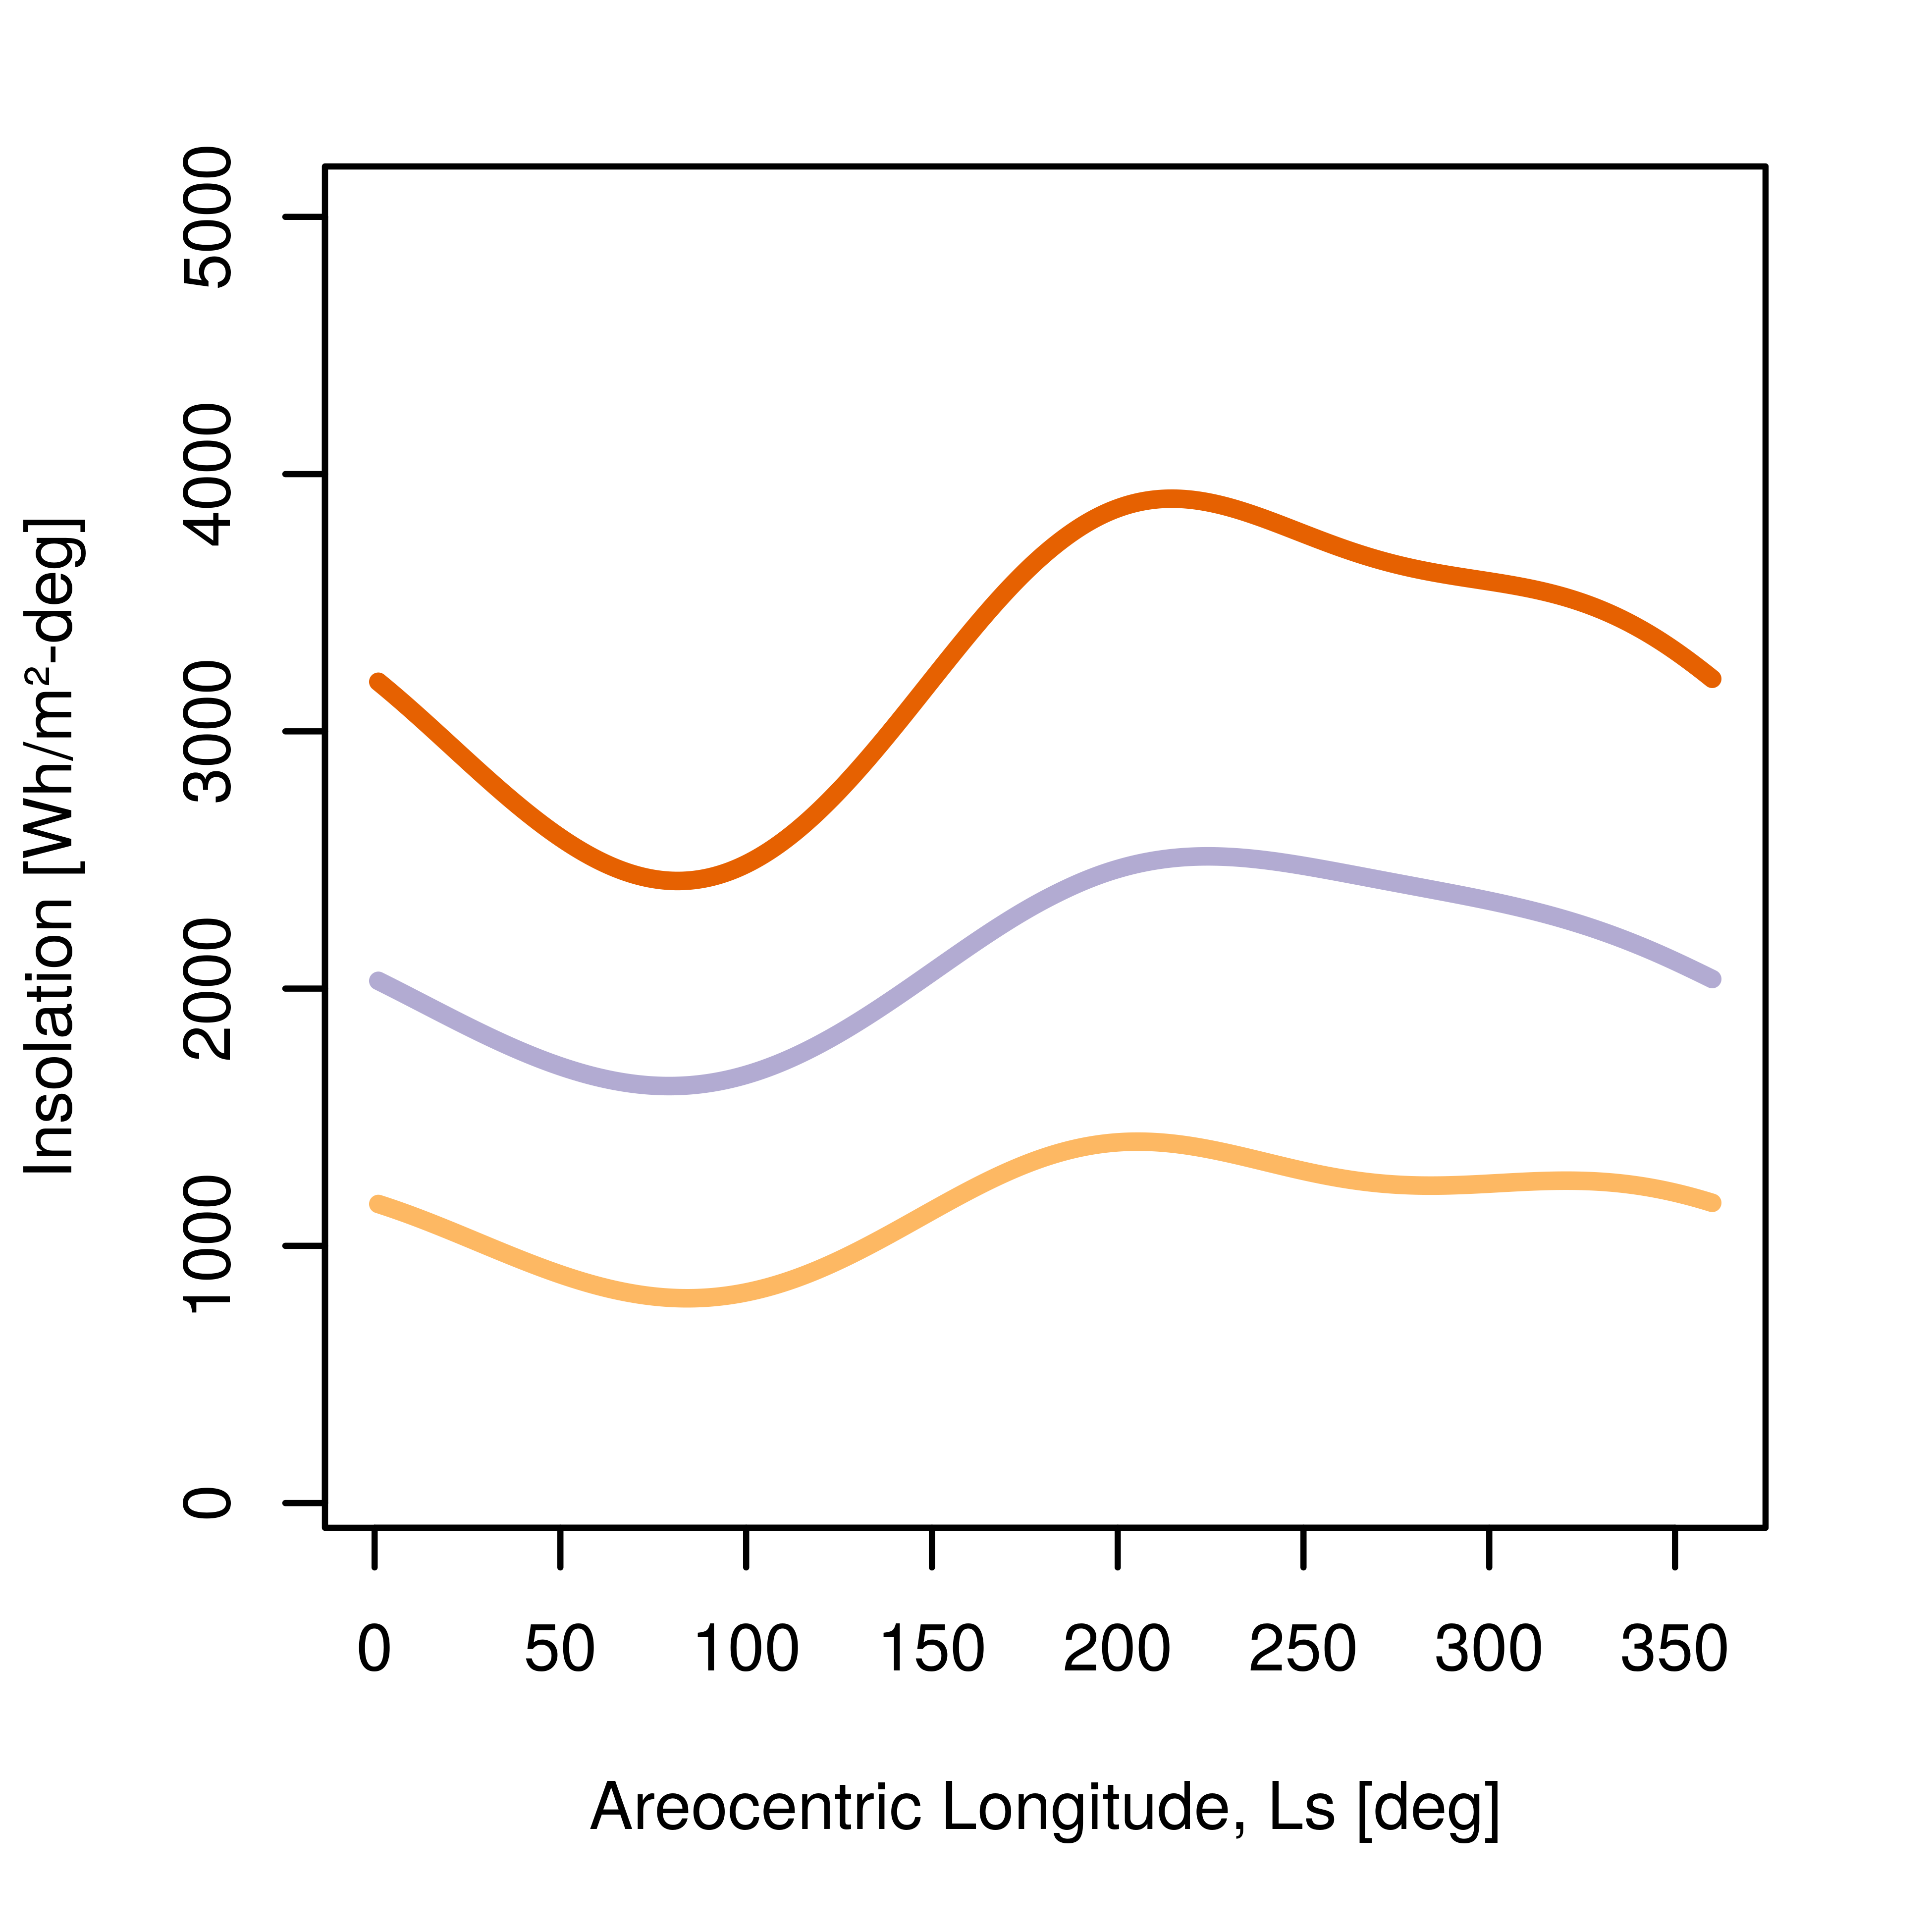
\includegraphics[height=\graphicsHeight]{sections/martian-environment/plots/hh-hbh-and-hdh-as-a-function-of-ls-for-tau1-phi205-and-albedo-027}
  		\subcaption{$\tau = 1$}
  		\label{fig:sub:insolation-ls-tau-factor-1}
  	\end{subfigure}\\[0.8ex]
%% 2nd row
    \begin{subfigure}[t]{\subfigureWidth}
      \centering
  		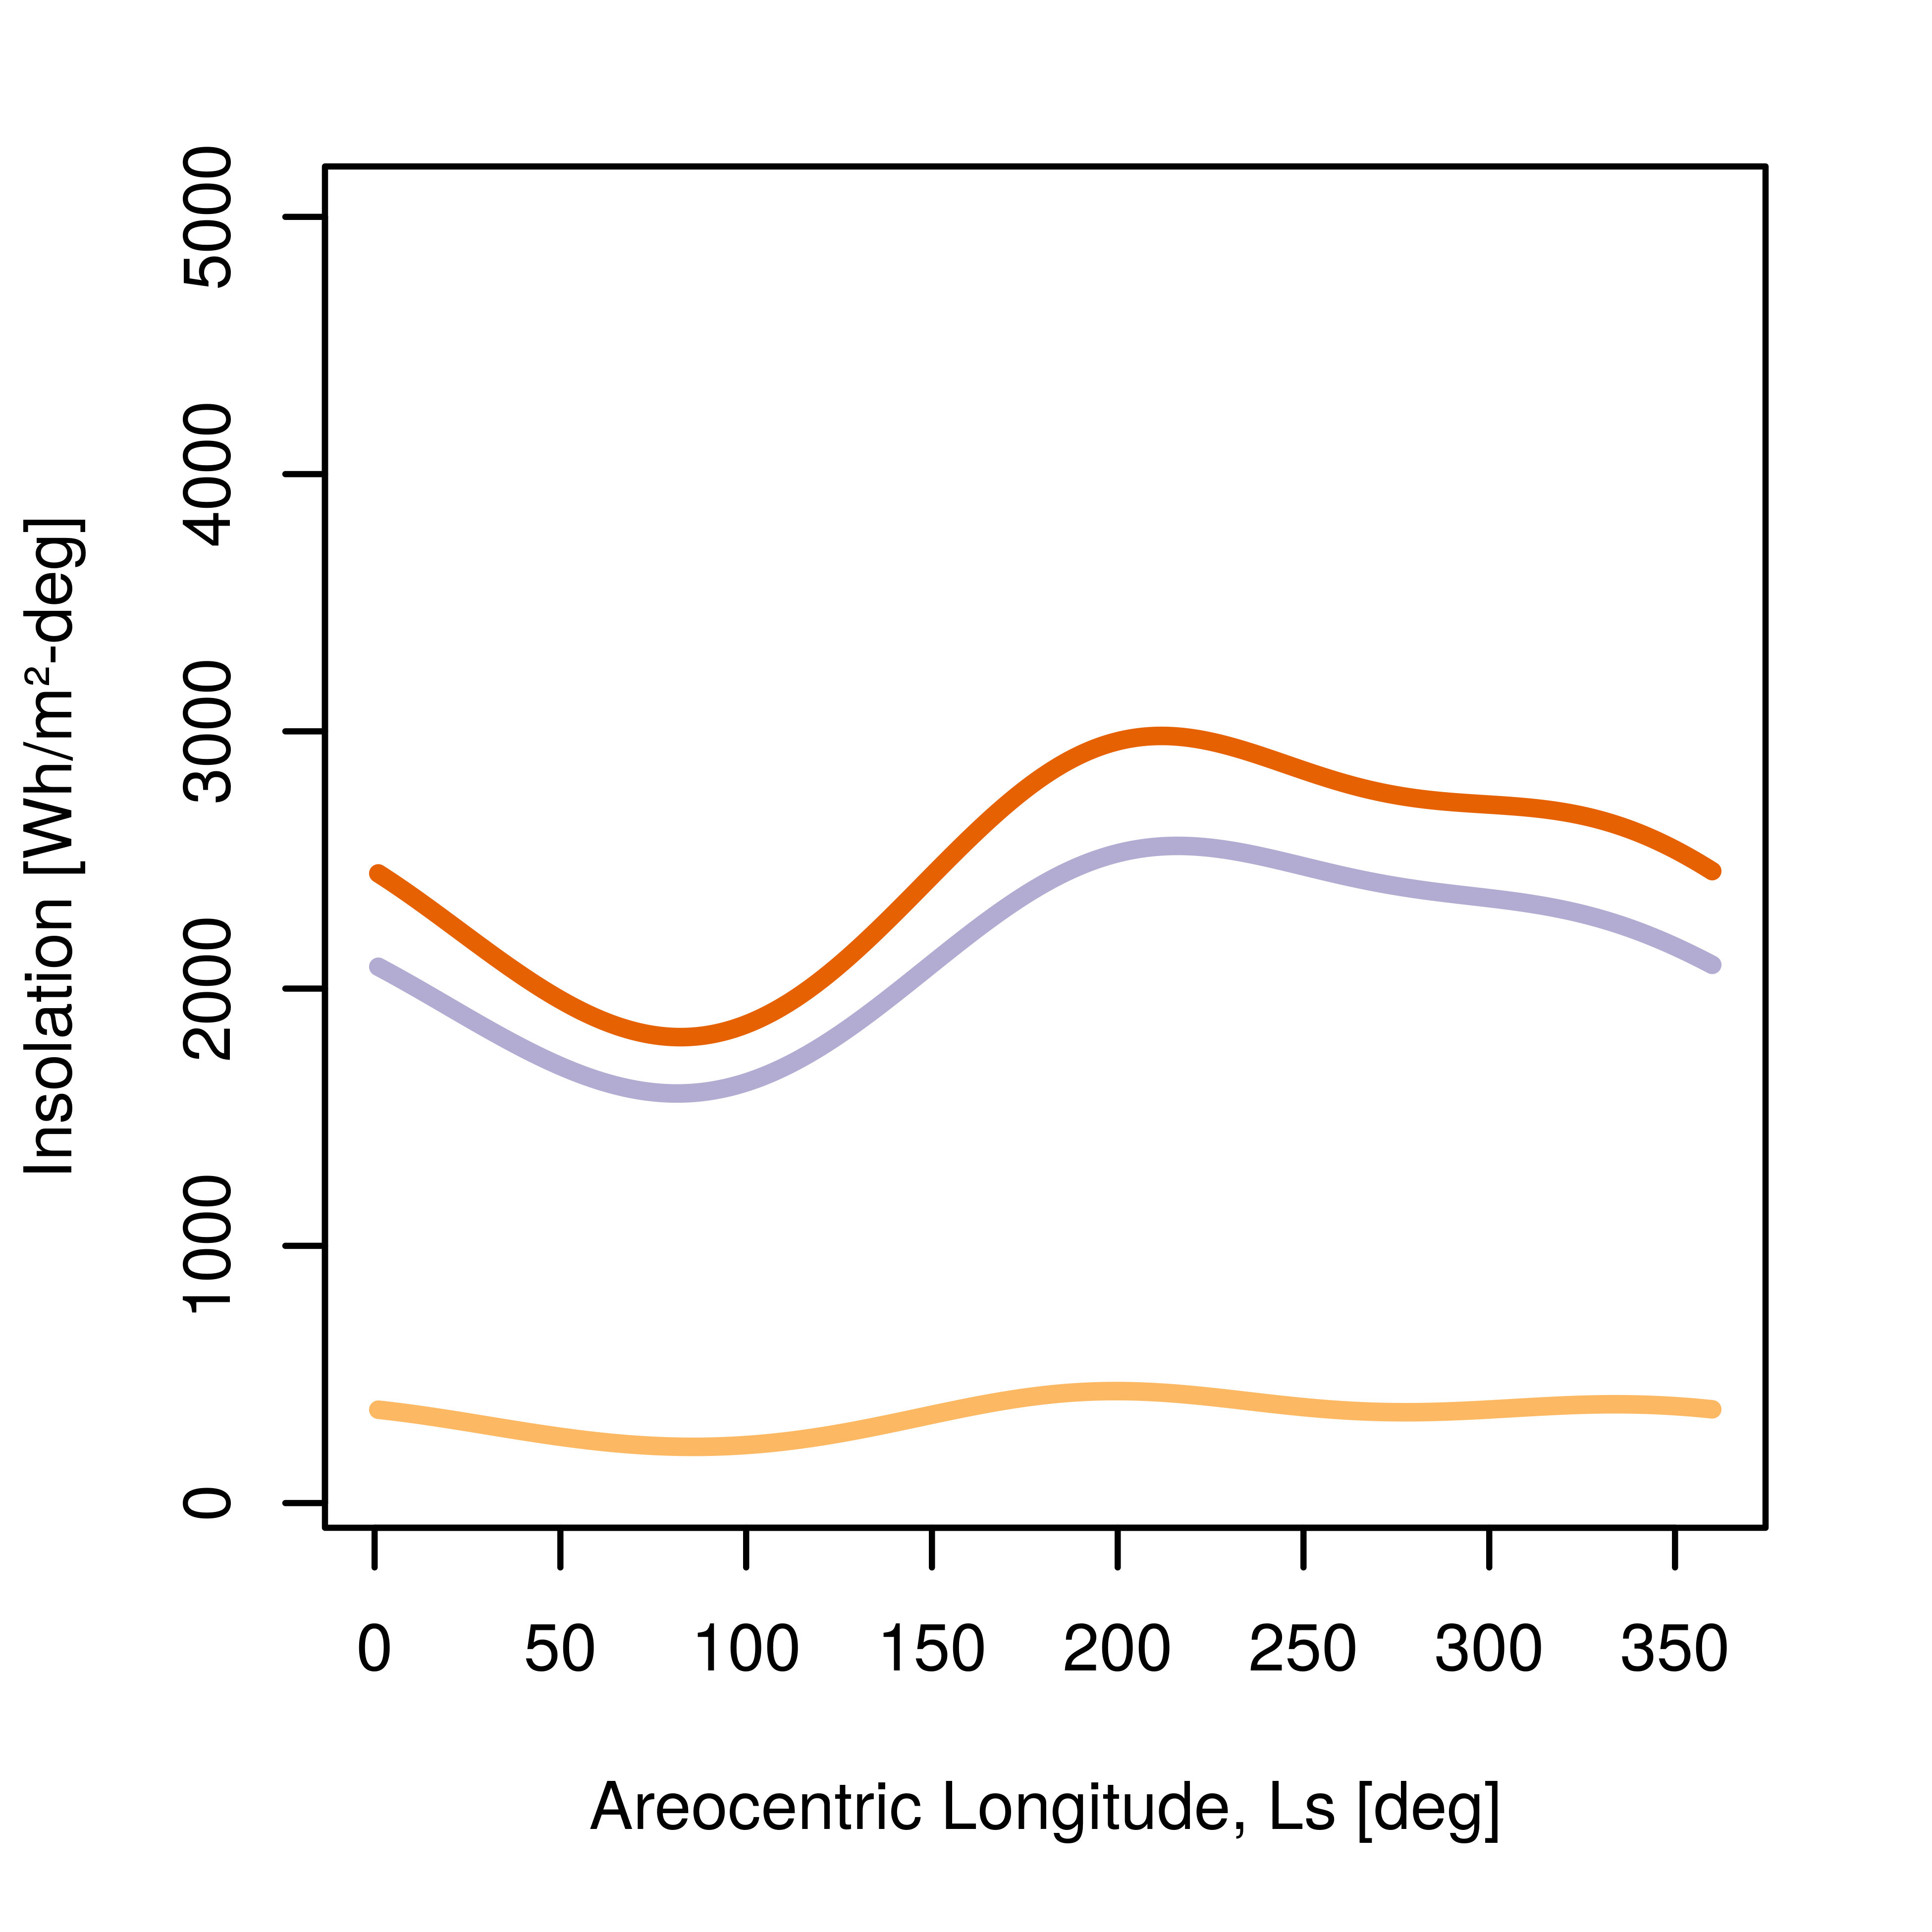
\includegraphics[height=\graphicsHeight]{sections/martian-environment/plots/hh-hbh-and-hdh-as-a-function-of-ls-for-tau2-phi205-and-albedo-027}
  		\subcaption{$\tau = 2$}
  		\label{fig:sub:insolation-ls-tau-factor-2}
  	\end{subfigure}\hfill
	   \begin{subfigure}[t]{\subfigureWidth}
      \centering
  		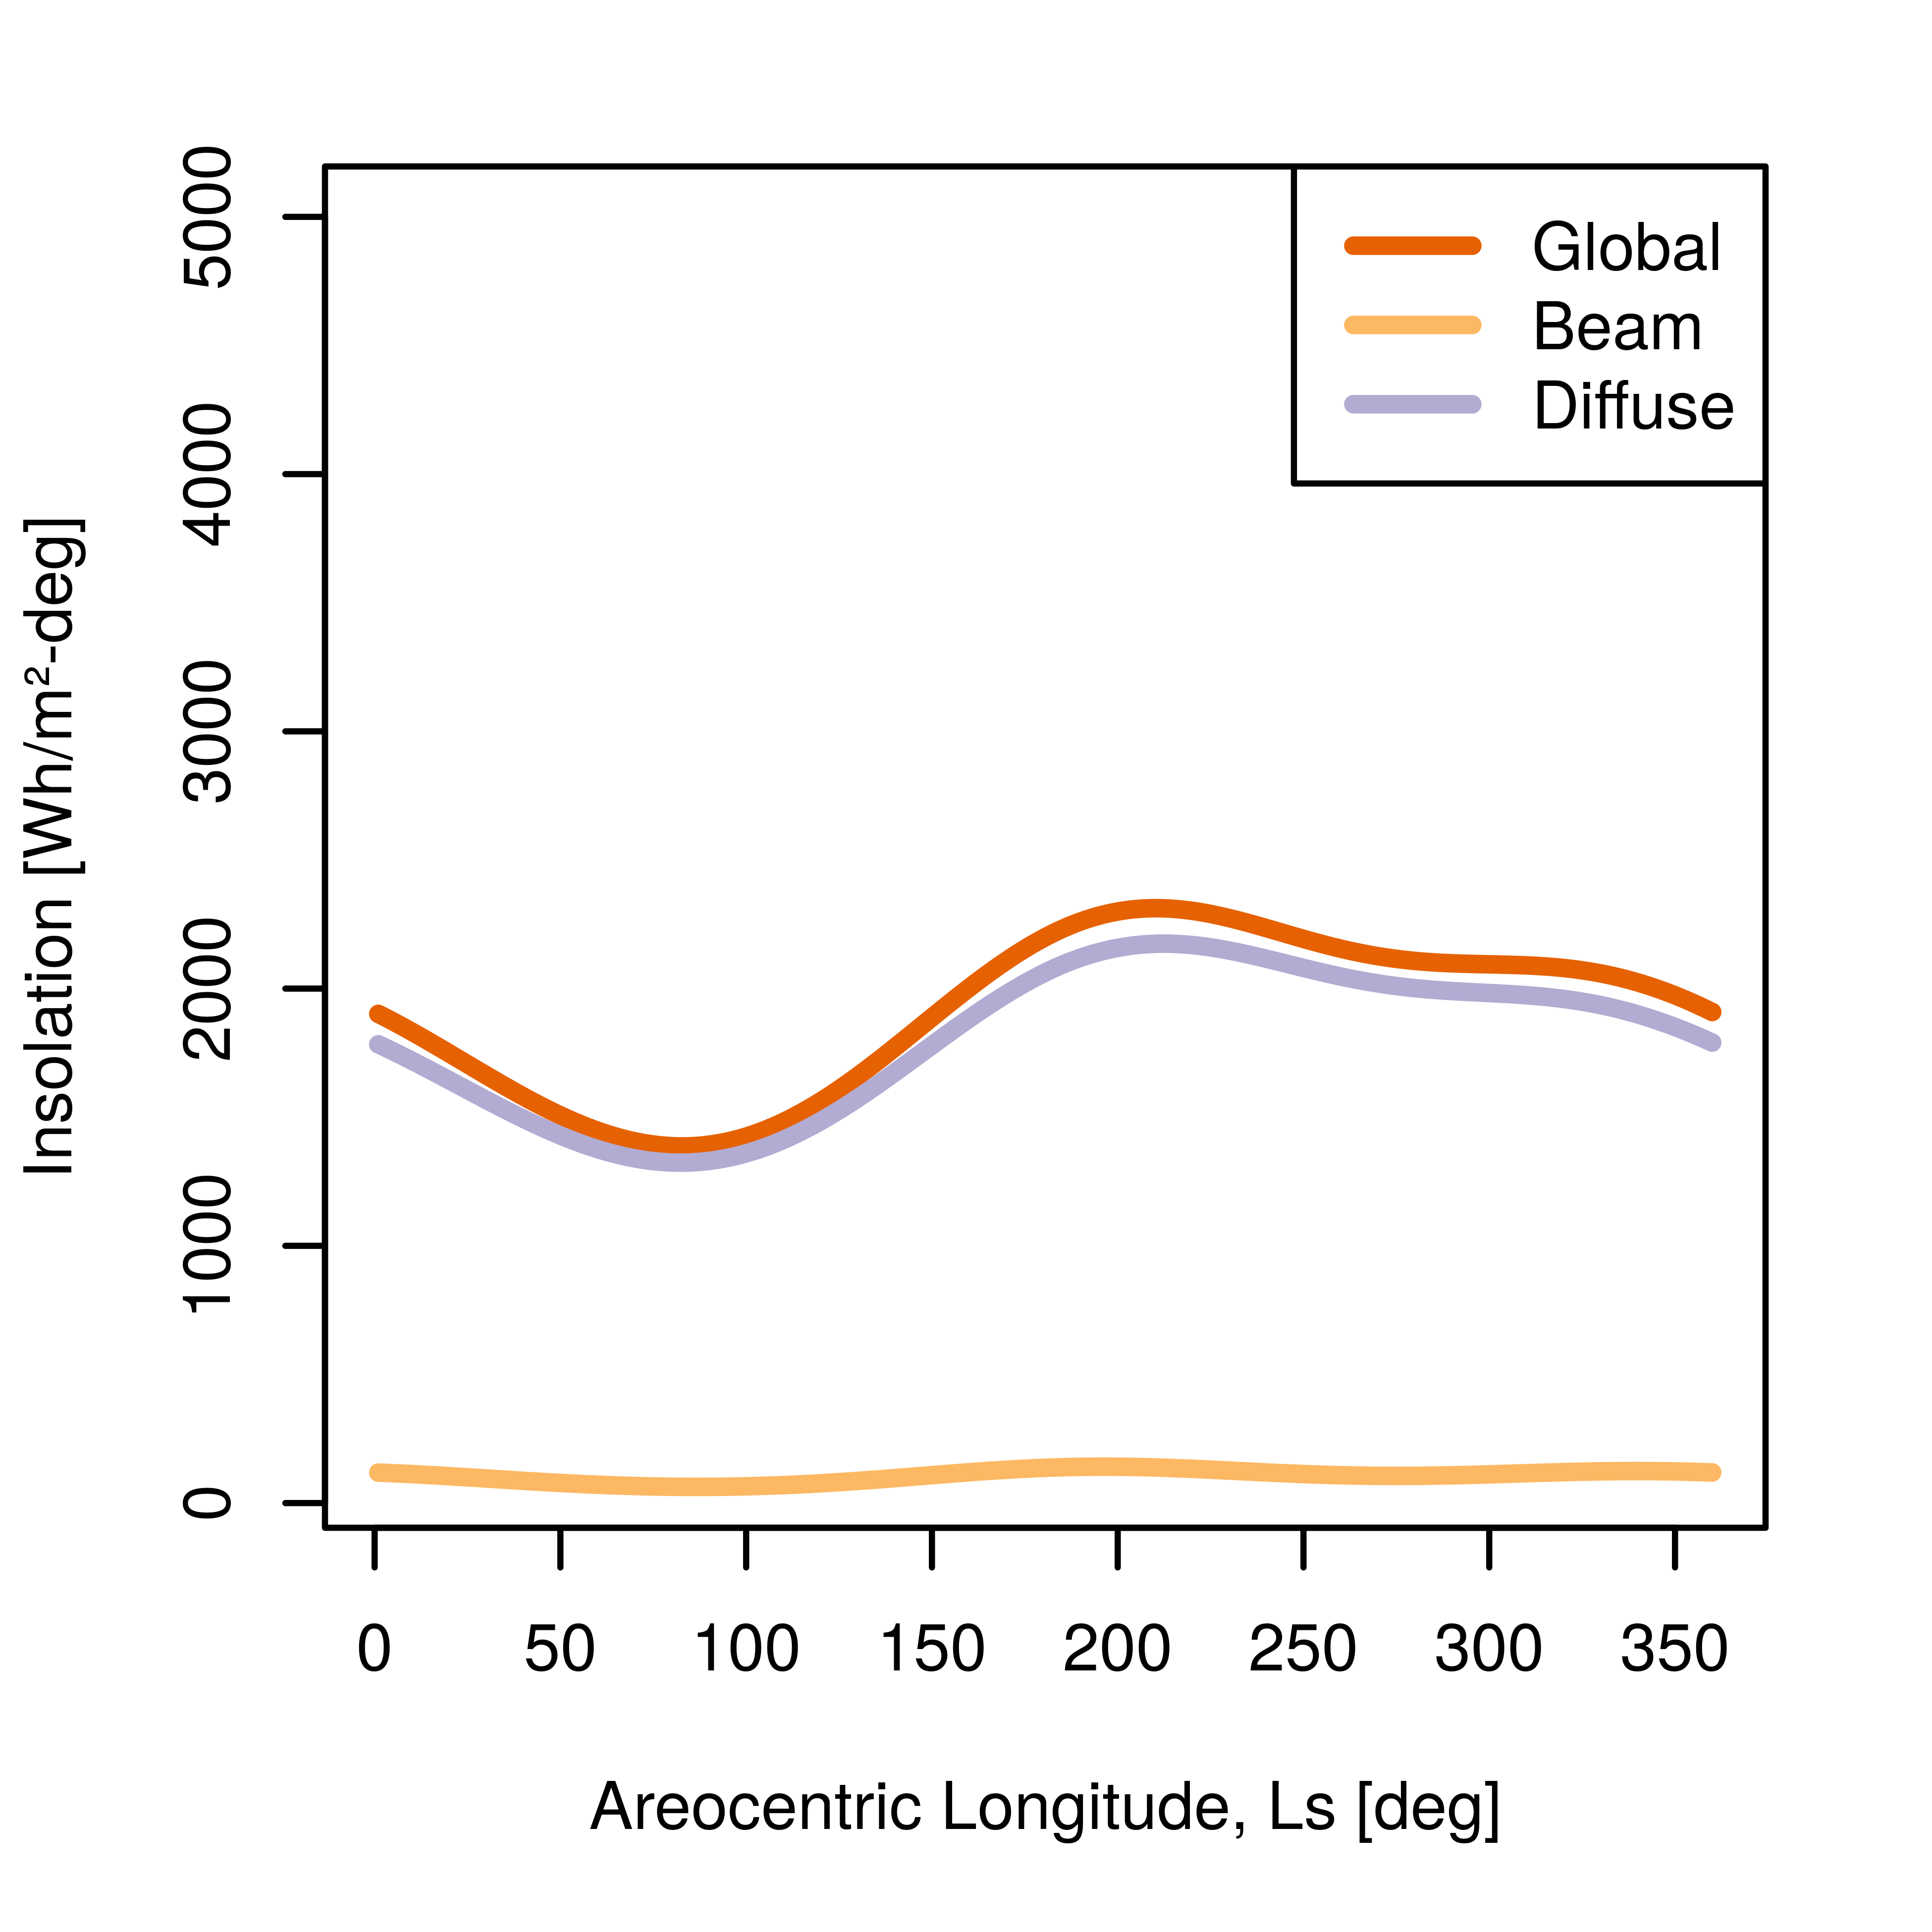
\includegraphics[height=\graphicsHeight]{sections/martian-environment/plots/hh-hbh-and-hdh-as-a-function-of-ls-for-tau3-phi205-and-albedo-027}
  		\subcaption{$\tau = 3$}
  		\label{fig:sub:insolation-ls-tau-factor-3}
	   \end{subfigure}\hfill
	\caption{Variation of global, beam, and diffuse insolation on Mars horizontal surface as a function of areocentric longitude at Endeavour Crater.}
	\label{fig:plot:insolation-ls}
\vspace{-2ex}
\end{figure}

Daily insolations are obtained when $\omega_1$ and $\omega_2$ are set for a time period between sunrise and sunset. The resulting values are denoted as $H_{h}$, $H_{bh}$, and $H_{dh}$ for global, beam, and diffuse insolations on Mars horizontal surface and $H_{obh}$ for a horizontal surface at the top of Mars atmosphere. Similarly to $I_{dh}$, the daily diffuse insolations $H_{dh}$ is obtained from the same relationship presented in Equation \ref{eq:G_h_1}.

To illustrate the variation of beam, direct, and diffuse insolations during a Martian day, a diurnal profile is presented in Figure \ref{fig:plot:insolation-phi} at different planetary latitudes during the aphelion for a clear day with $\tau = 0.5$. The seasonal influences are evident: at $L_{s} = \SI{71}{\degree}$, it is Autumn in the northern hemisphere and insolations at $\phi = \SI{20}{\degree}$ are much greater than those in the southern hemisphere at $\phi = \SI{-20}{\degree}$ and $\phi = \SI{-40}{\degree}$. Furthermore, daylight at $\phi = \SI{20}{\degree}$ spans across 16 hours whereas they only last for 12 hours at $\phi = \SI{-20}{\degree}$ and 10 hours at $\phi = \SI{-40}{\degree}$ .


\begin{figure}[H]
\captionsetup[subfigure]{justification=centering}
\vspace{-2ex}
	\centering
    %% setup sizes
    \setlength{\subfigureWidth}{0.50\textwidth}
    \setlength{\graphicsHeight}{80mm}
    %% kill hyper-link highlighting
    \hypersetup{hidelinks=true}%
    %% the figures
%% 1st row
  	\begin{subfigure}[t]{\subfigureWidth}
      \centering
  		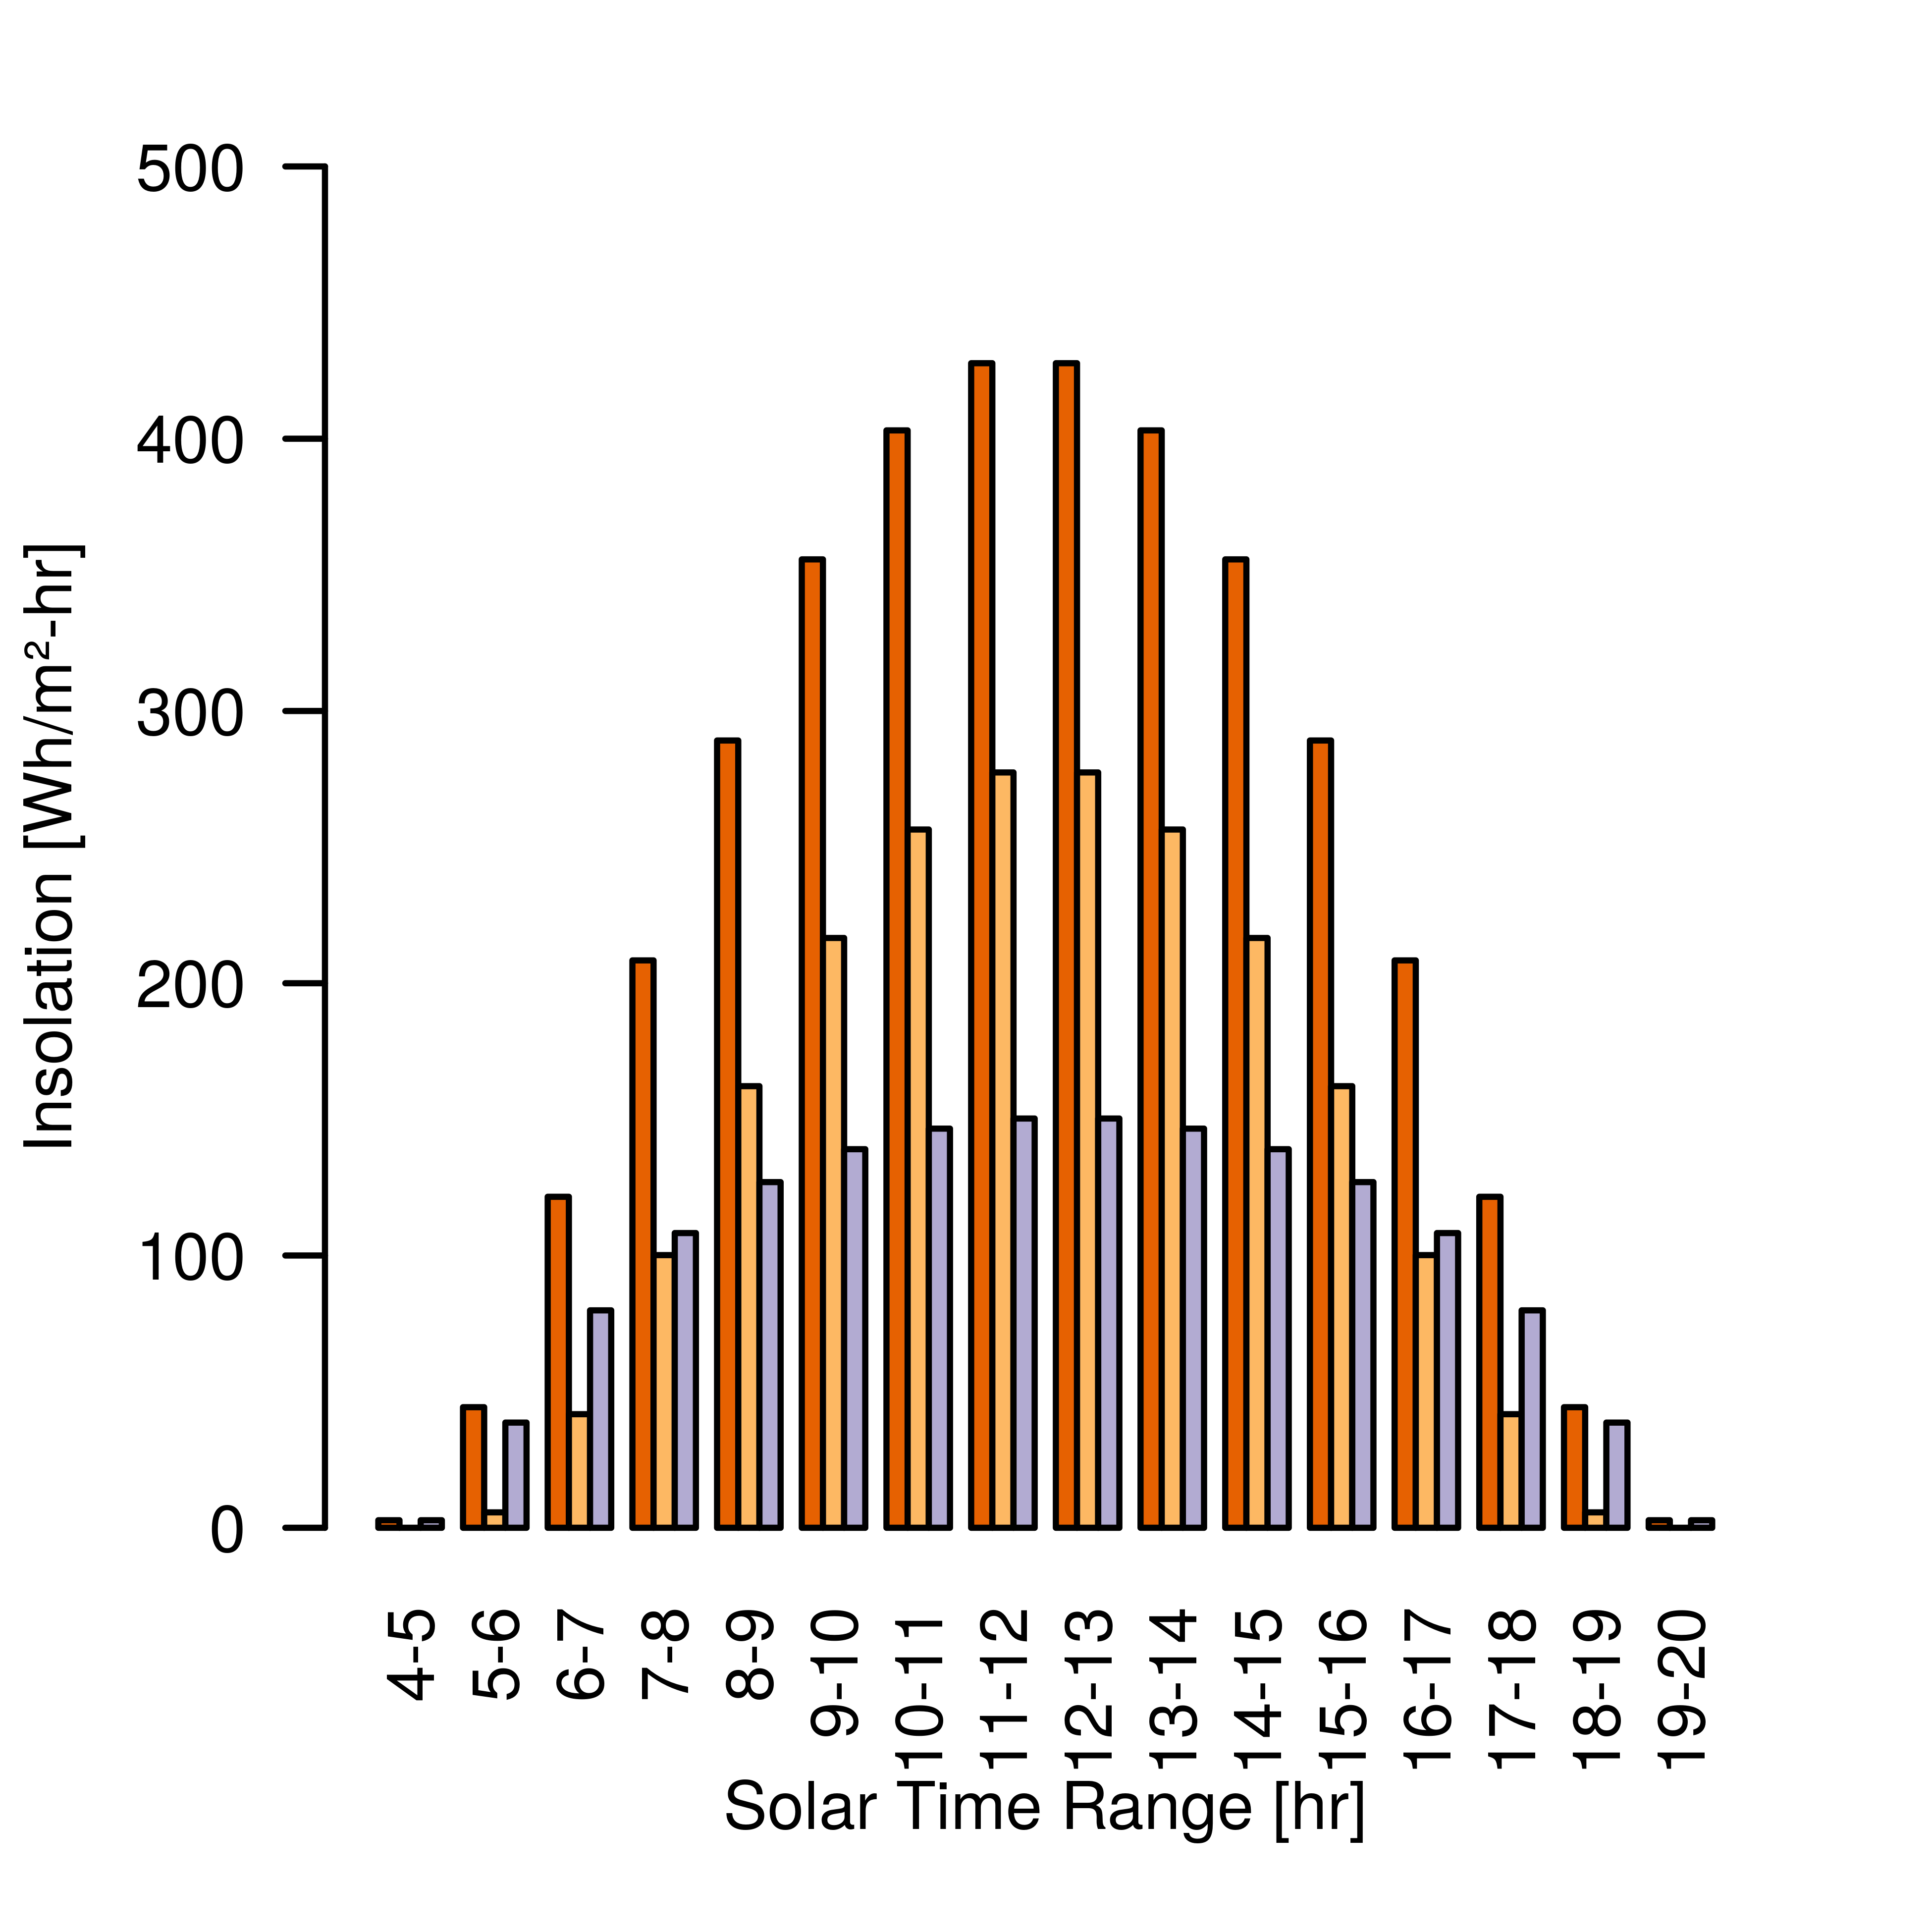
\includegraphics[height=\graphicsHeight]{sections/martian-environment/plots/ih-ibh-and-idh-variation-1-for-ls-71-phi-40-tau-05-and-albedo-027}
  		\subcaption{$\phi = \SI{40}{\degree}$}
  		\label{fig:sub:insolation-phi-m40}
  	\end{subfigure}\hfill
    \begin{subfigure}[t]{\subfigureWidth}
      \centering
  		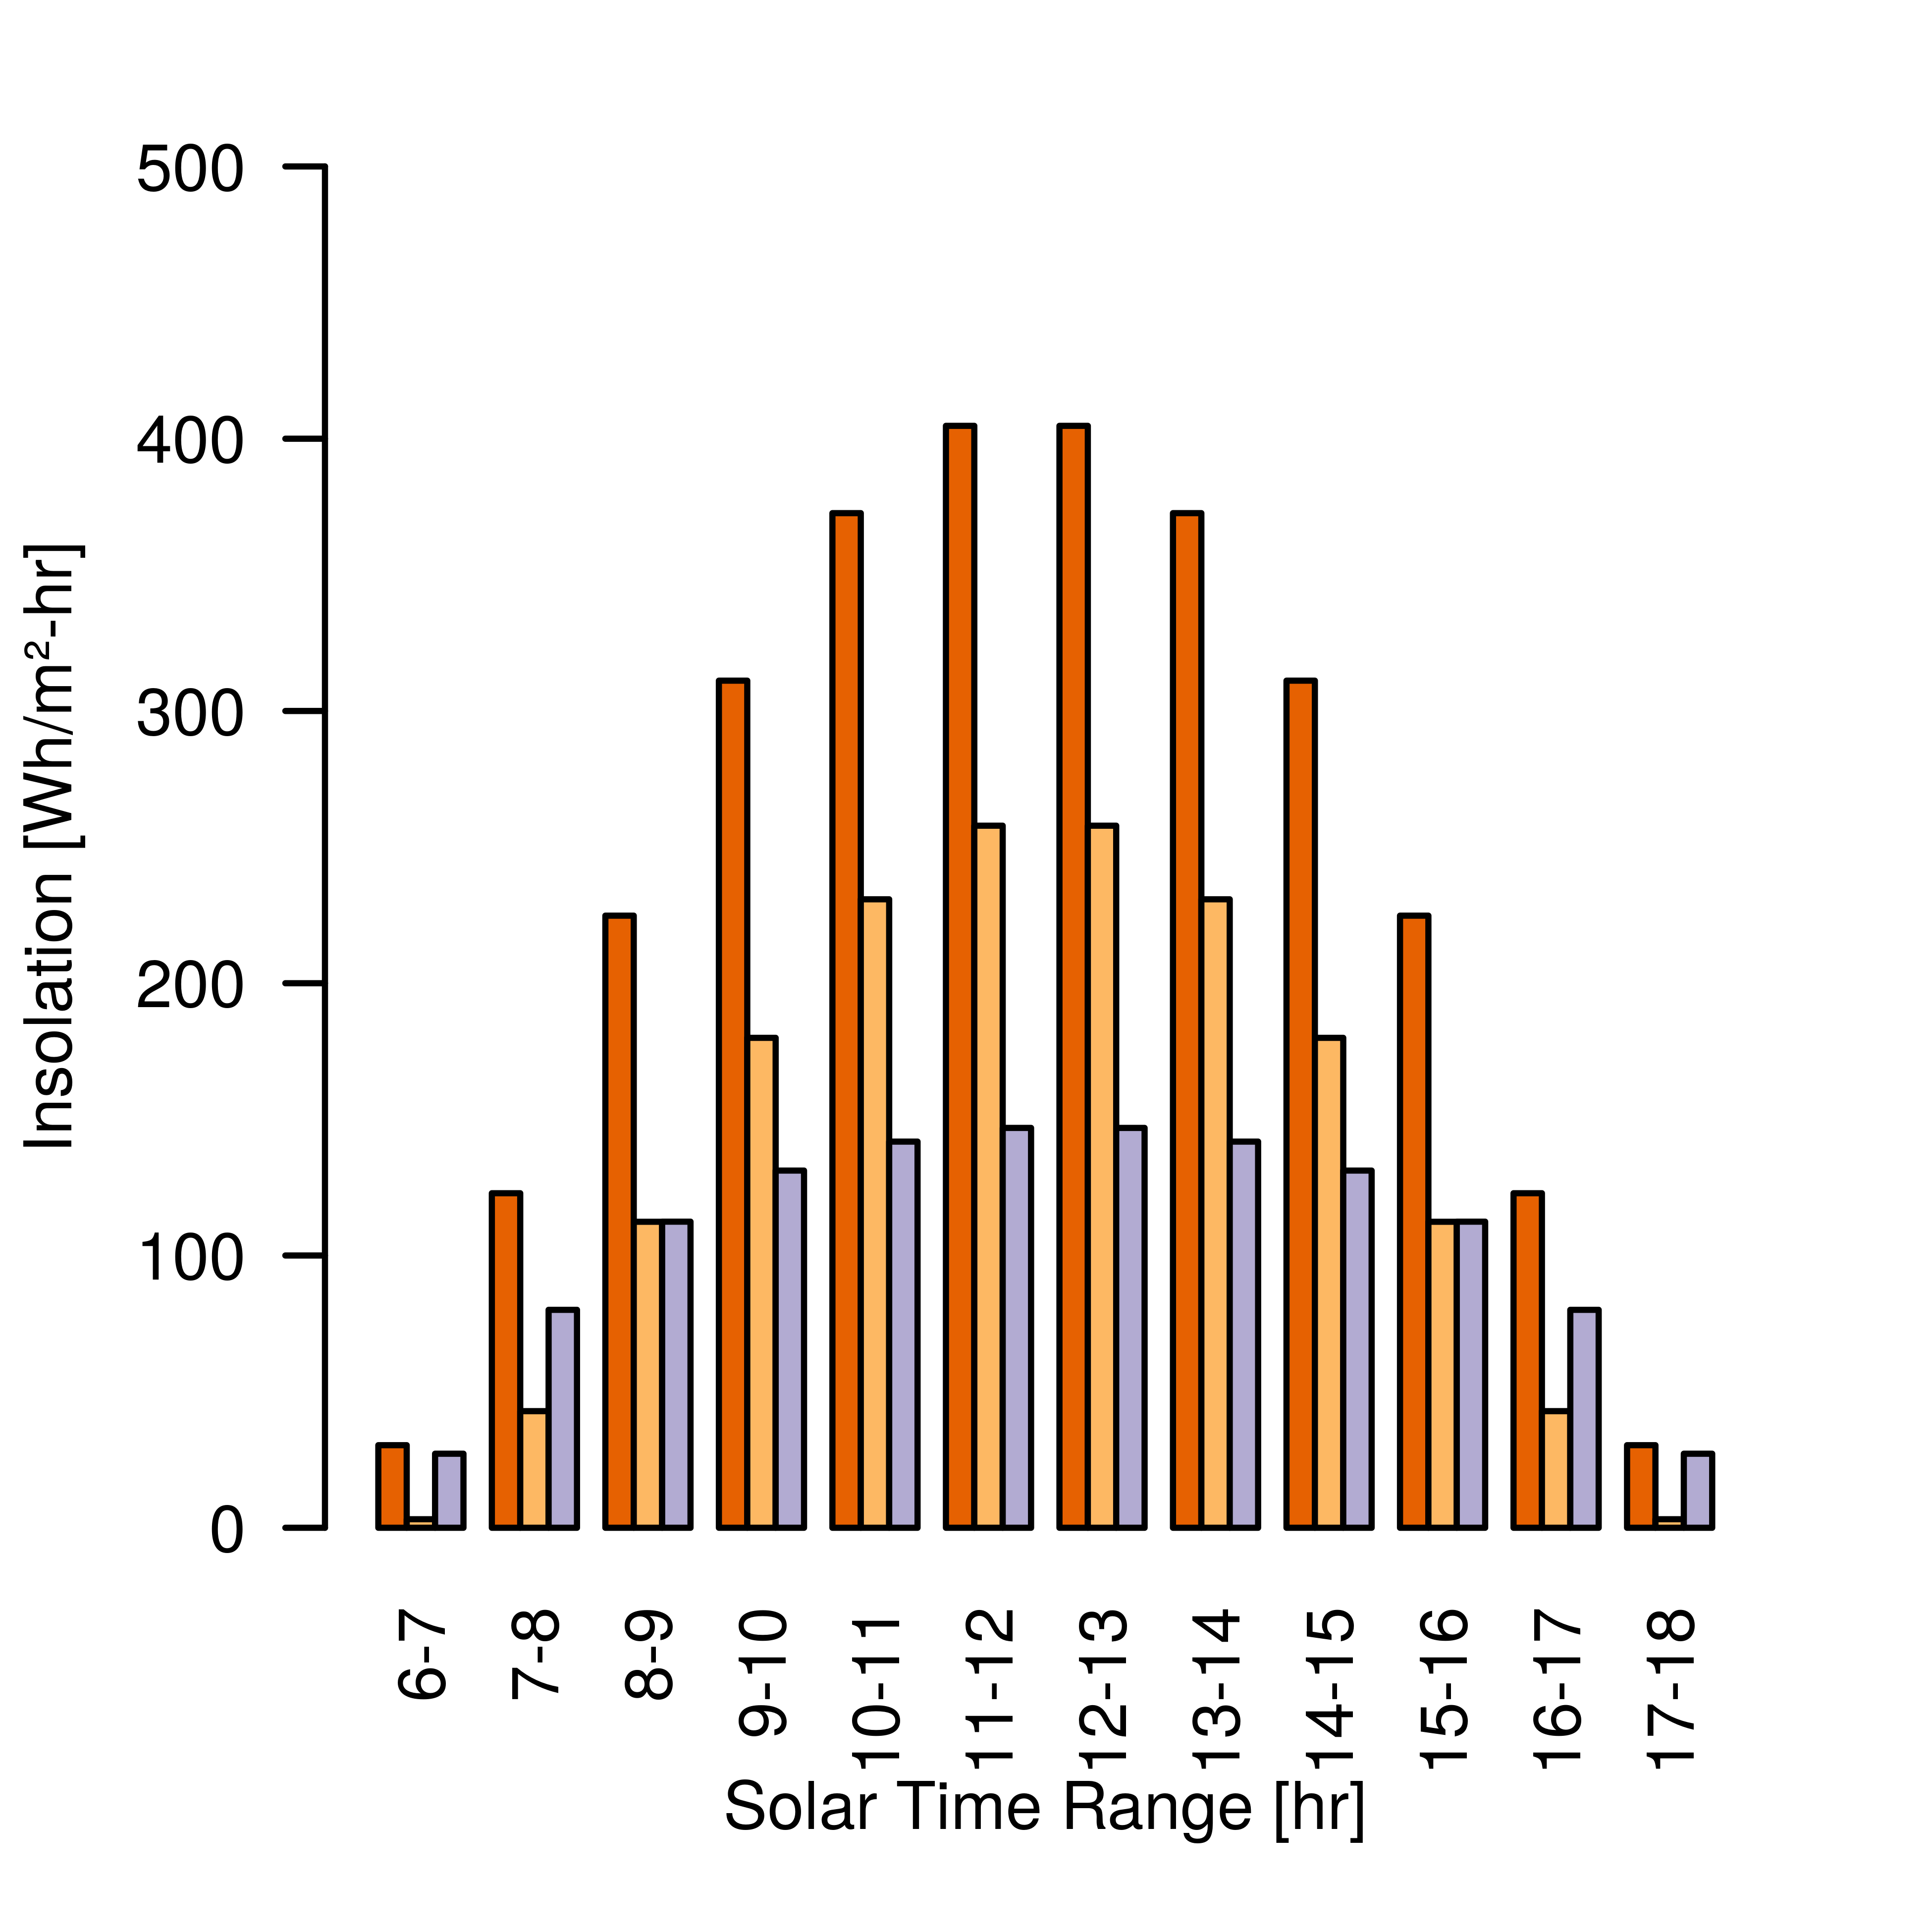
\includegraphics[height=\graphicsHeight]{sections/martian-environment/plots/ih-ibh-and-idh-variation-2-for-ls-71-phi-0-tau-05-and-albedo-027}
  		\subcaption{$\phi = \SI{0}{\degree}$}
  		\label{fig:sub:insolation-phi-m20}
  	\end{subfigure}\\[0.8ex]
%% 2nd row
    \begin{subfigure}[t]{\subfigureWidth}
      \centering
  		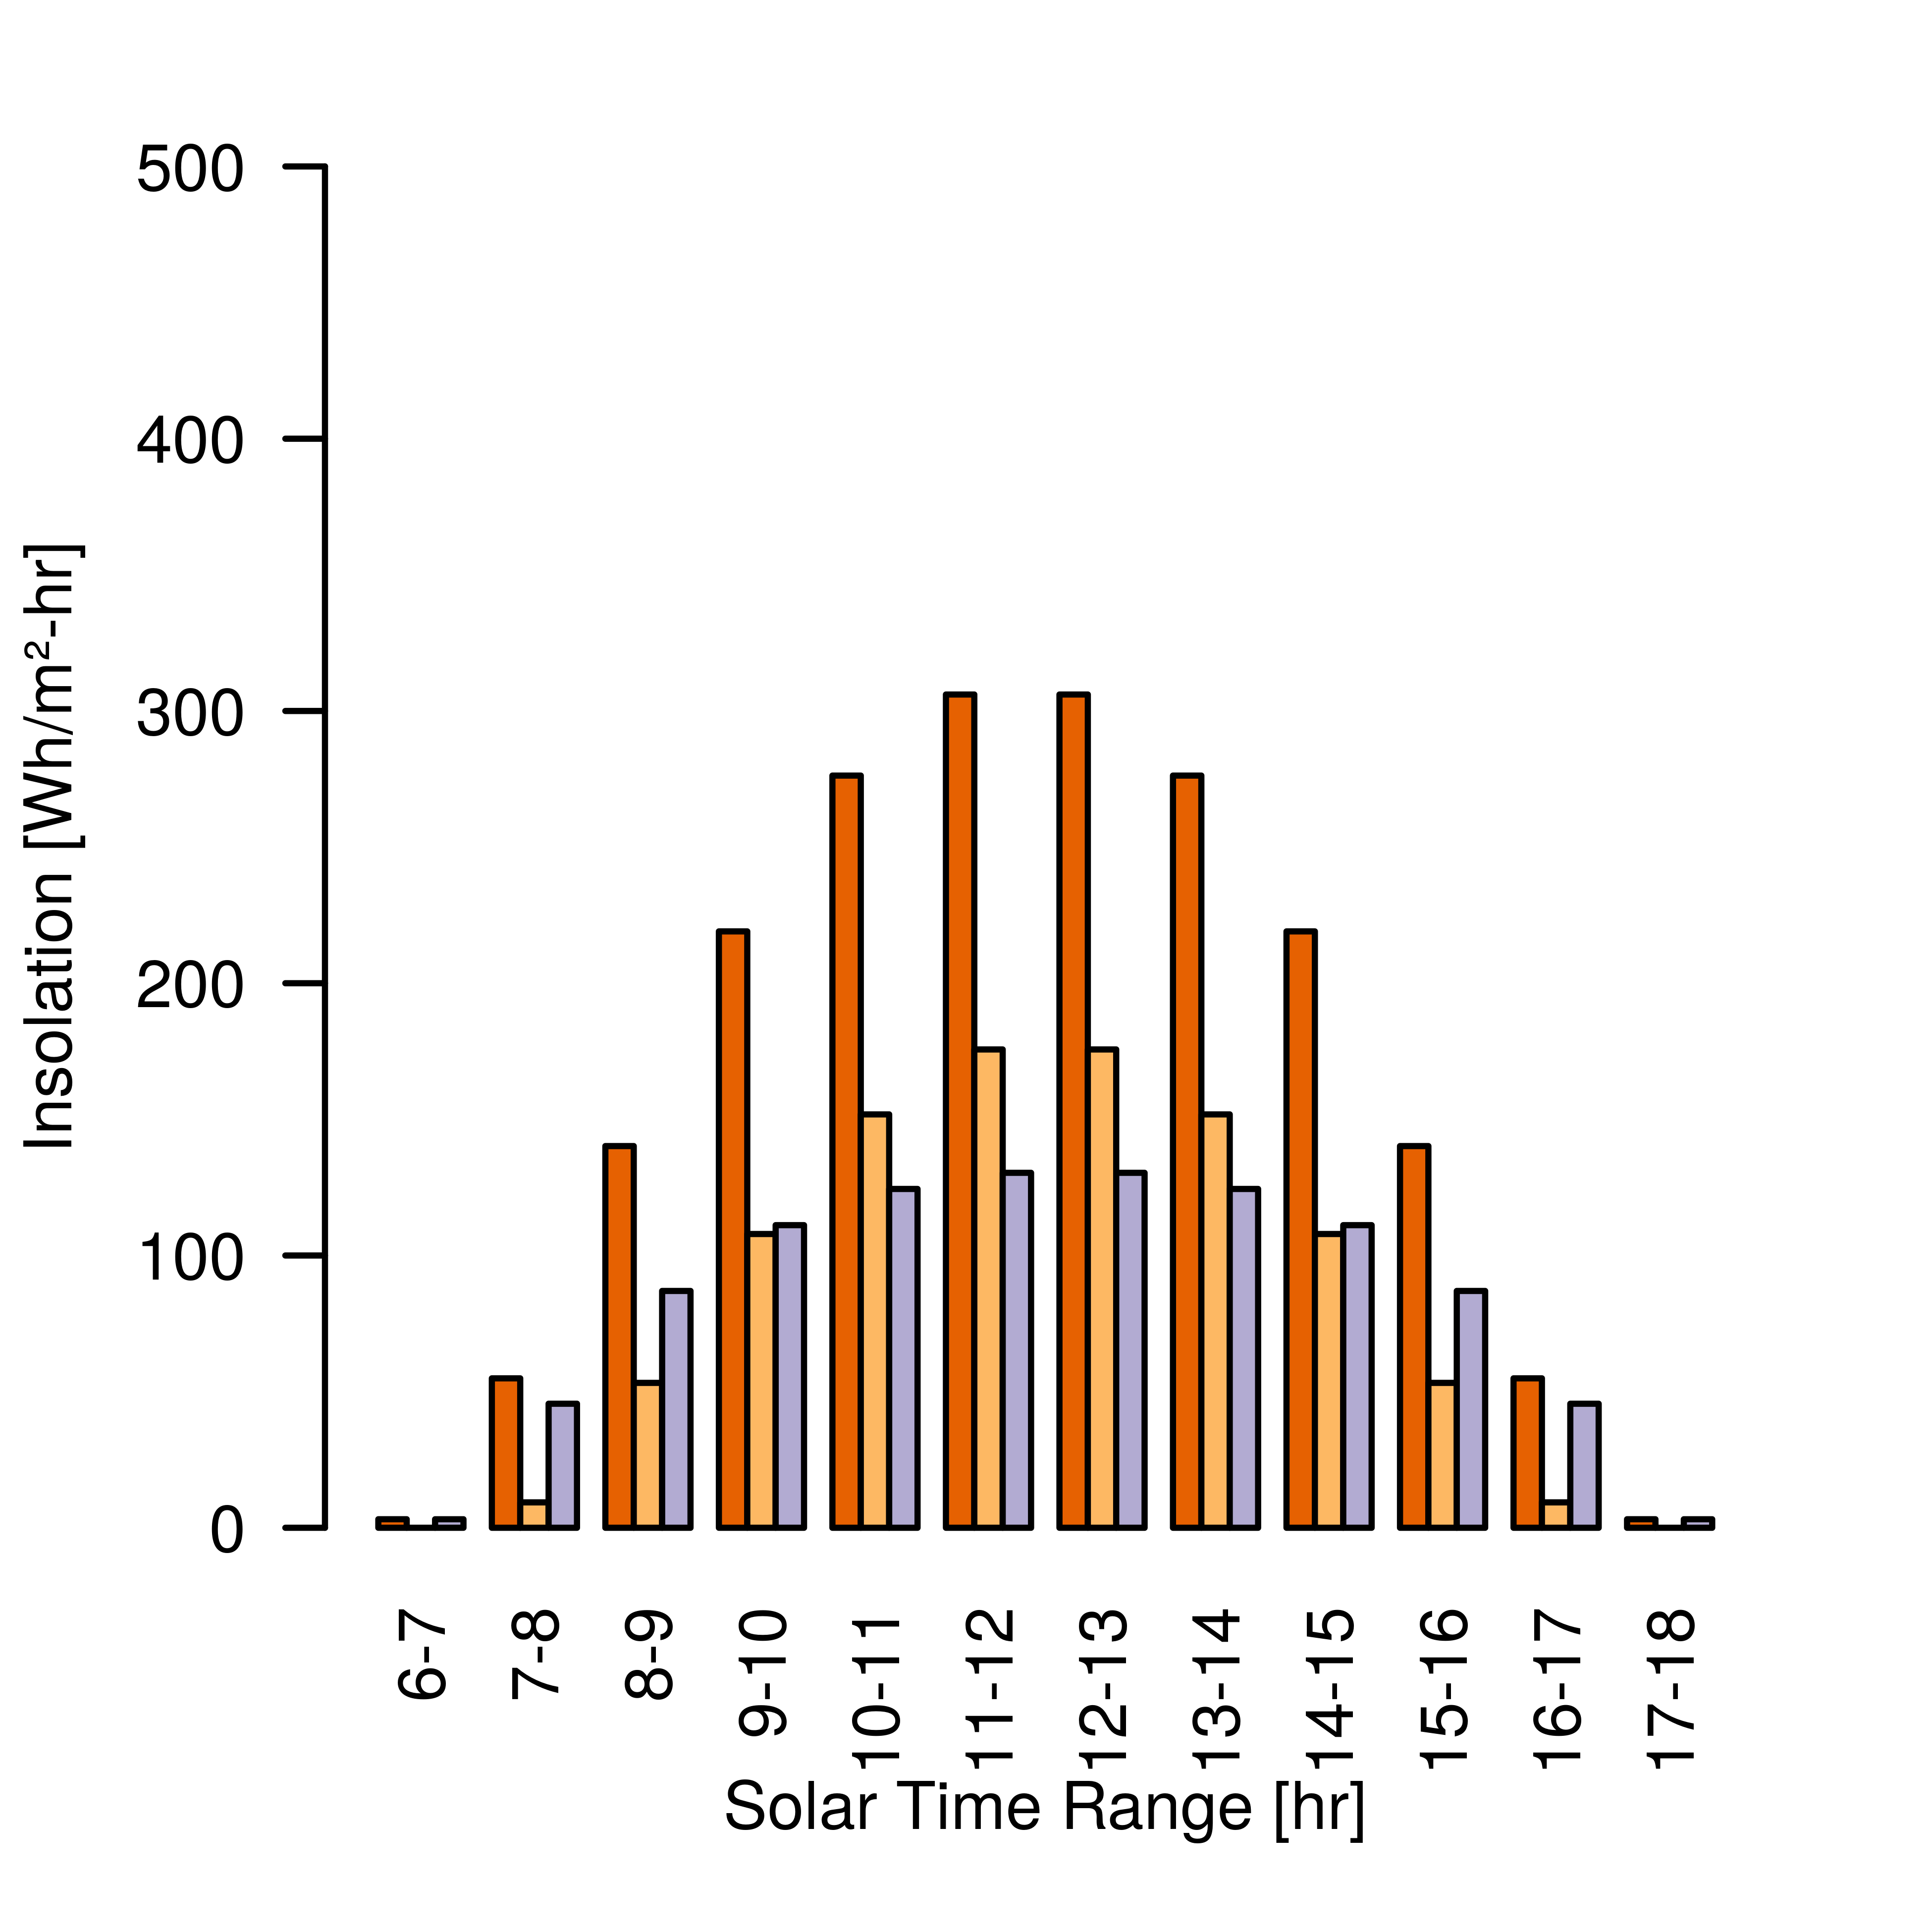
\includegraphics[height=\graphicsHeight]{sections/martian-environment/plots/ih-ibh-and-idh-variation-3-for-ls-71-phi-20-tau-05-and-albedo-027}
  		\subcaption{$\phi = \SI{-20}{\degree}$}
  		\label{fig:sub:insolation-phi-0}
  	\end{subfigure}\hfill
	   \begin{subfigure}[t]{\subfigureWidth}
      \centering
  		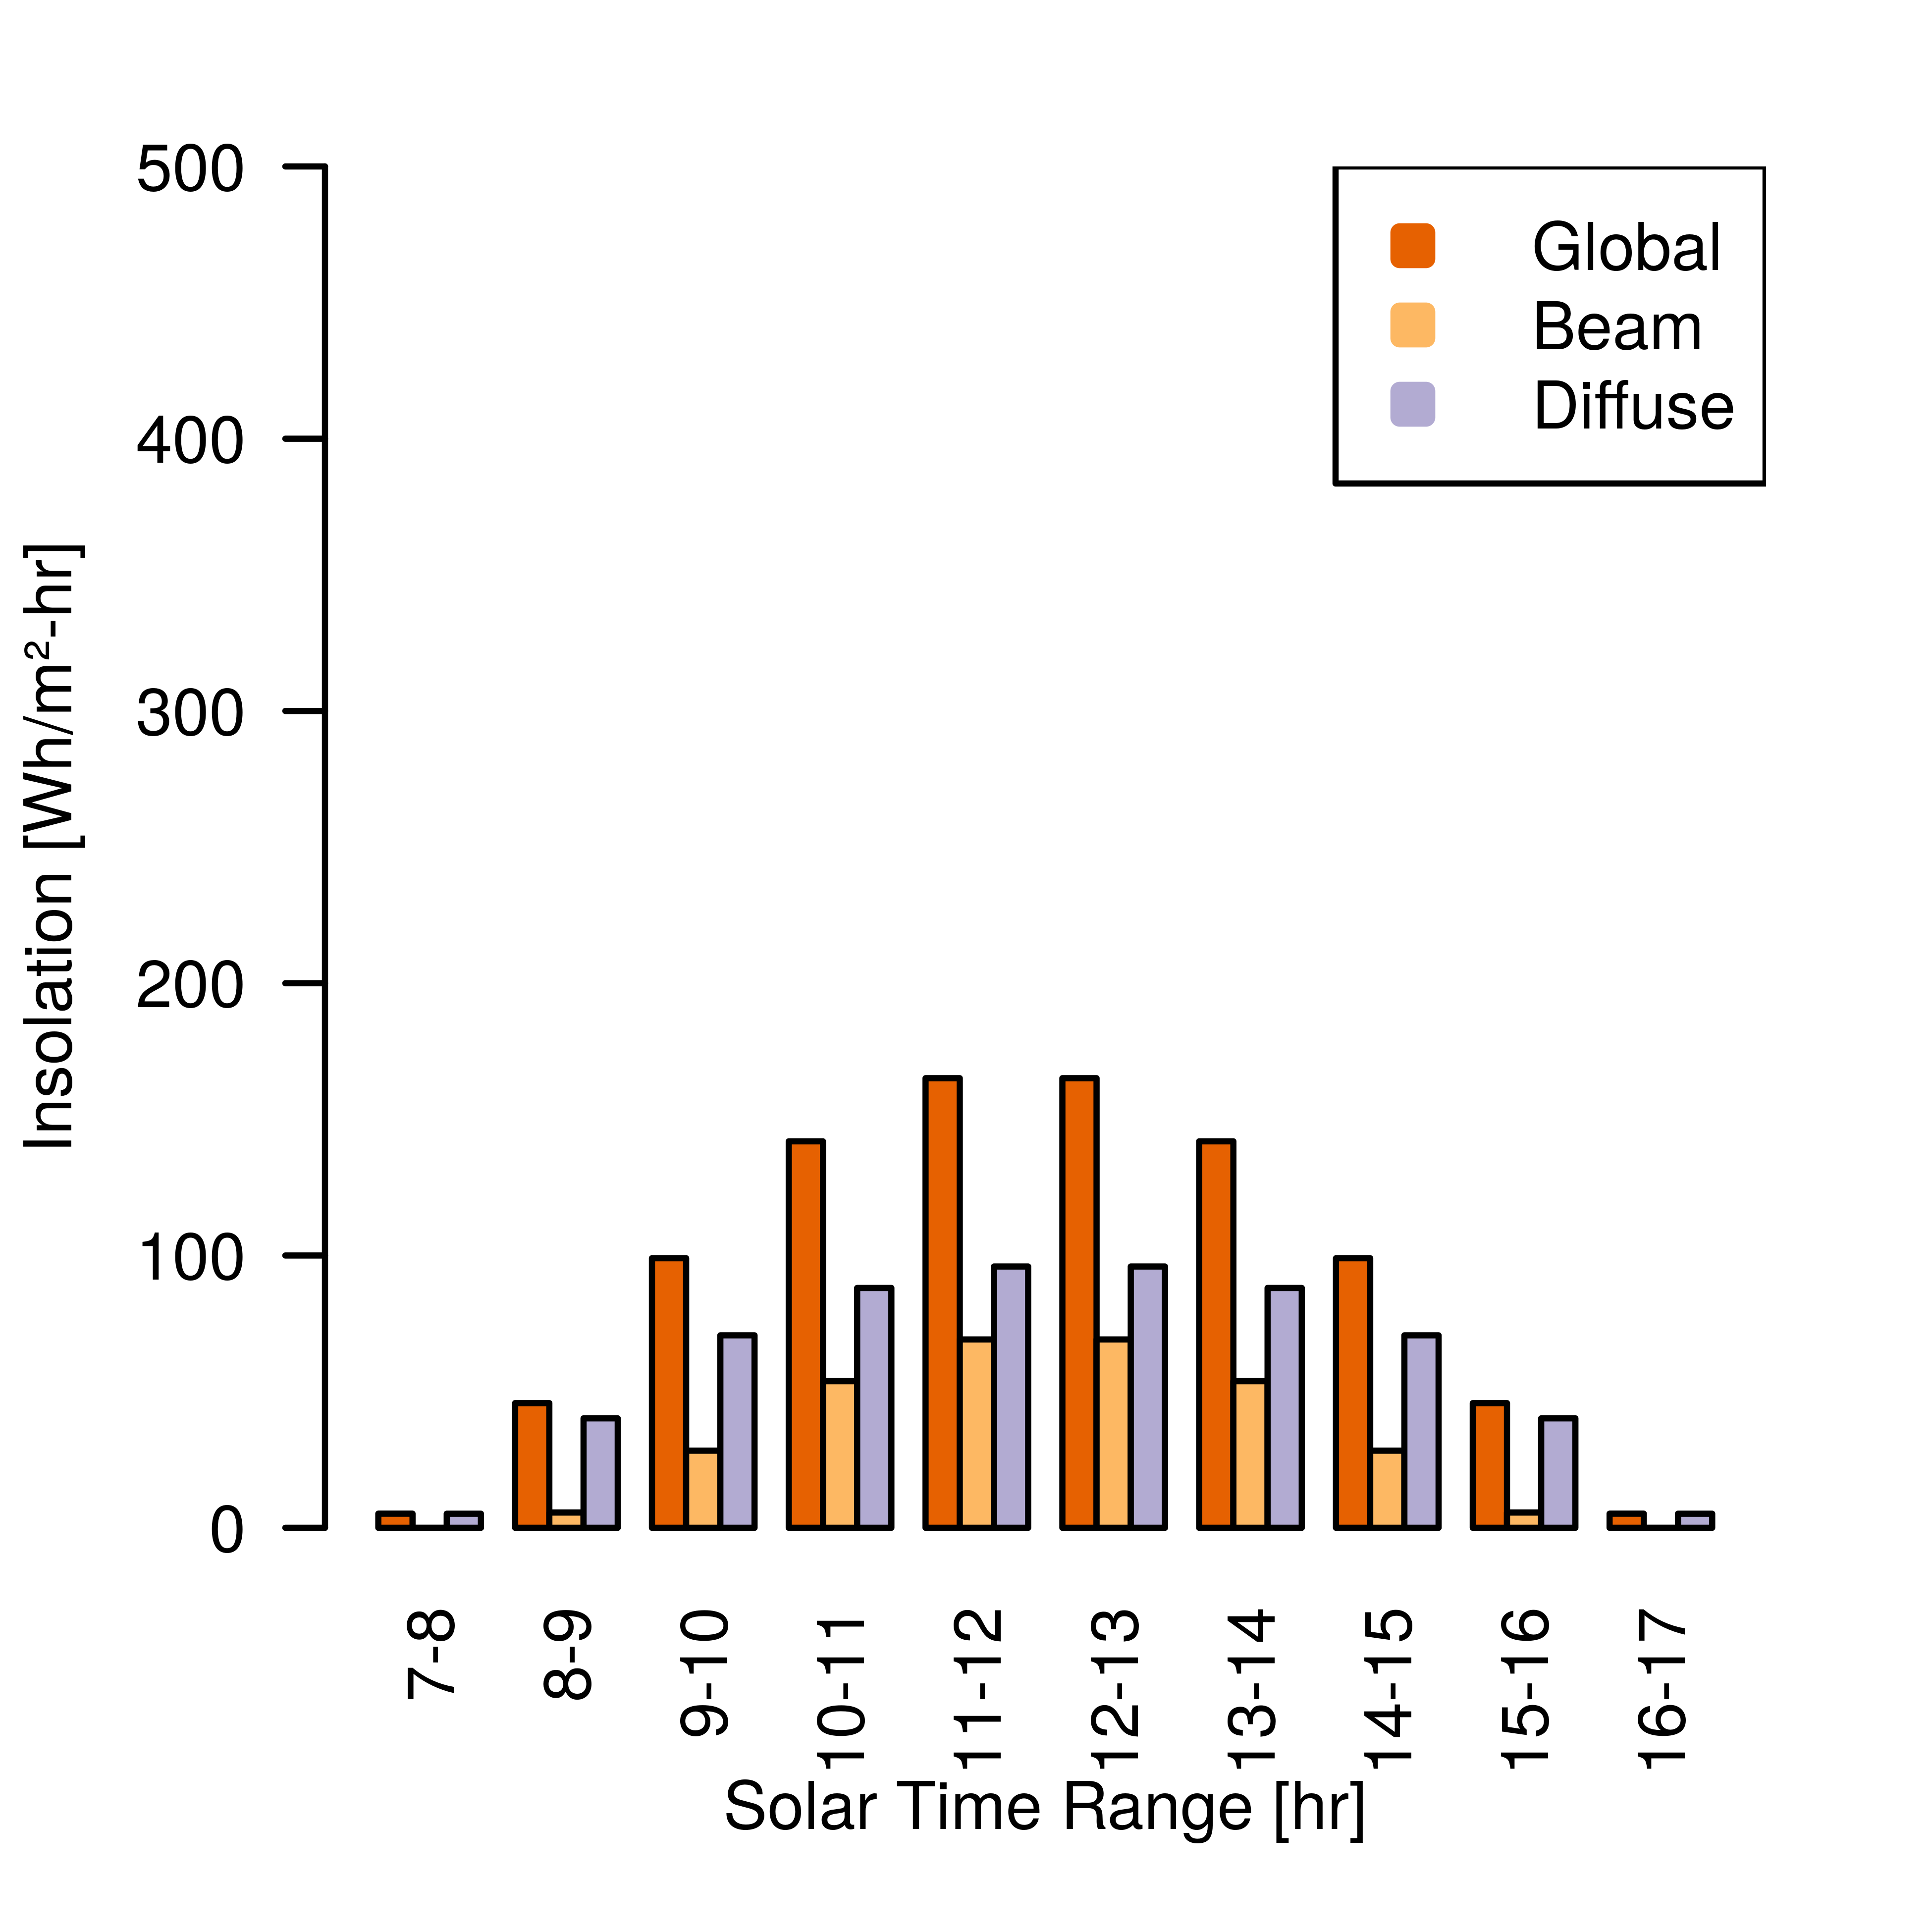
\includegraphics[height=\graphicsHeight]{sections/martian-environment/plots/ih-ibh-and-idh-variation-4-for-ls-71-phi-40-tau-05-and-albedo-027}
  		\subcaption{$\phi = \SI{-40}{\degree}$}
  		\label{fig:sub:insolation-phi-p20}
	   \end{subfigure}\hfill
	\caption{Diurnal variation of global, beam, and diffuse insolation on Mars horizontal surface at different planetary latitudes.}
	\label{fig:plot:insolation-phi}
\vspace{-2ex}
\end{figure}

\subsection{Inclined Surface}
\label{sec:MartianEnvironment:SolarRadiation:InclinedSurface}

Hitherto the irradiance and insolation calculations on the surface of Mars have been restricted to a horizontal plane. However, scenarios with descent and ascent profiles such as with the topographic slope variation in crater exploration missions make it necessary to consider solar radiation received on inclined surfaces.

\subsubsection{Irradiance}
\label{sec:MartianEnvironment:SolarRadiation:InclinedSurface:Irradiance}

Global irradiance $G_{\beta}$ on an inclined surface can be obtained when parametizing the slope angle $\beta$ and the Sun angle of incidence $\theta$ \citemarsenv{Appelbaum1994}:

\begin{equation}
  \label{eq:G_beta}
  G_{\beta} = G_{b}\cos{\theta} + G_{dh}\cos{(\frac{\beta}{2})}^2 + al G_{h} \sin{(\frac{\beta}{2})}^2
\end{equation}

where and $al$ is the albedo.

The Sun angle of incidence itself is a function of the Sun zenith angle $z$ for the time of day, the slope angle $\beta$ for the inclination, and the solar azimuth $\gamma_{s}$ as well as the Sun surface azimuth angle $\gamma_{c}$ for the orientation of the inclination \citemarsenv{Appelbaum1994}:

\begin{equation}
  \label{eq:costheta}
  \cos{\theta} = \cos{\beta}\cos{z} +  \sin{\beta}\sin{z}\cos{(\gamma_{s} - \gamma_{c})}
\end{equation}

where the Sun zenith angle is given by \ref{eq:cosz}.

Variation of the global irradiance at the perihelion for different inclination angles are presented in Figure \ref{fig:plot:irradiance-inclined-gamma-c} for South, East, North, and West slope orientations. The influence of the inclination angle is most noticeable for a \SI{20}{\degree} slope oriented southwards resulting in a stronger irradiance profile than all other showcased slope angle and orientation configurations.

\ref{fig:plot:irradiance-inclined-gamma-c}

\begin{figure}[H]
\captionsetup[subfigure]{justification=centering}
\vspace{-2ex}
	\centering
    %% setup sizes
    \setlength{\subfigureWidth}{0.50\textwidth}
    \setlength{\graphicsHeight}{80mm}
    %% kill hyper-link highlighting
    \hypersetup{hidelinks=true}%
    %% the figures
%% 1st row
  	\begin{subfigure}[t]{\subfigureWidth}
      \centering
  		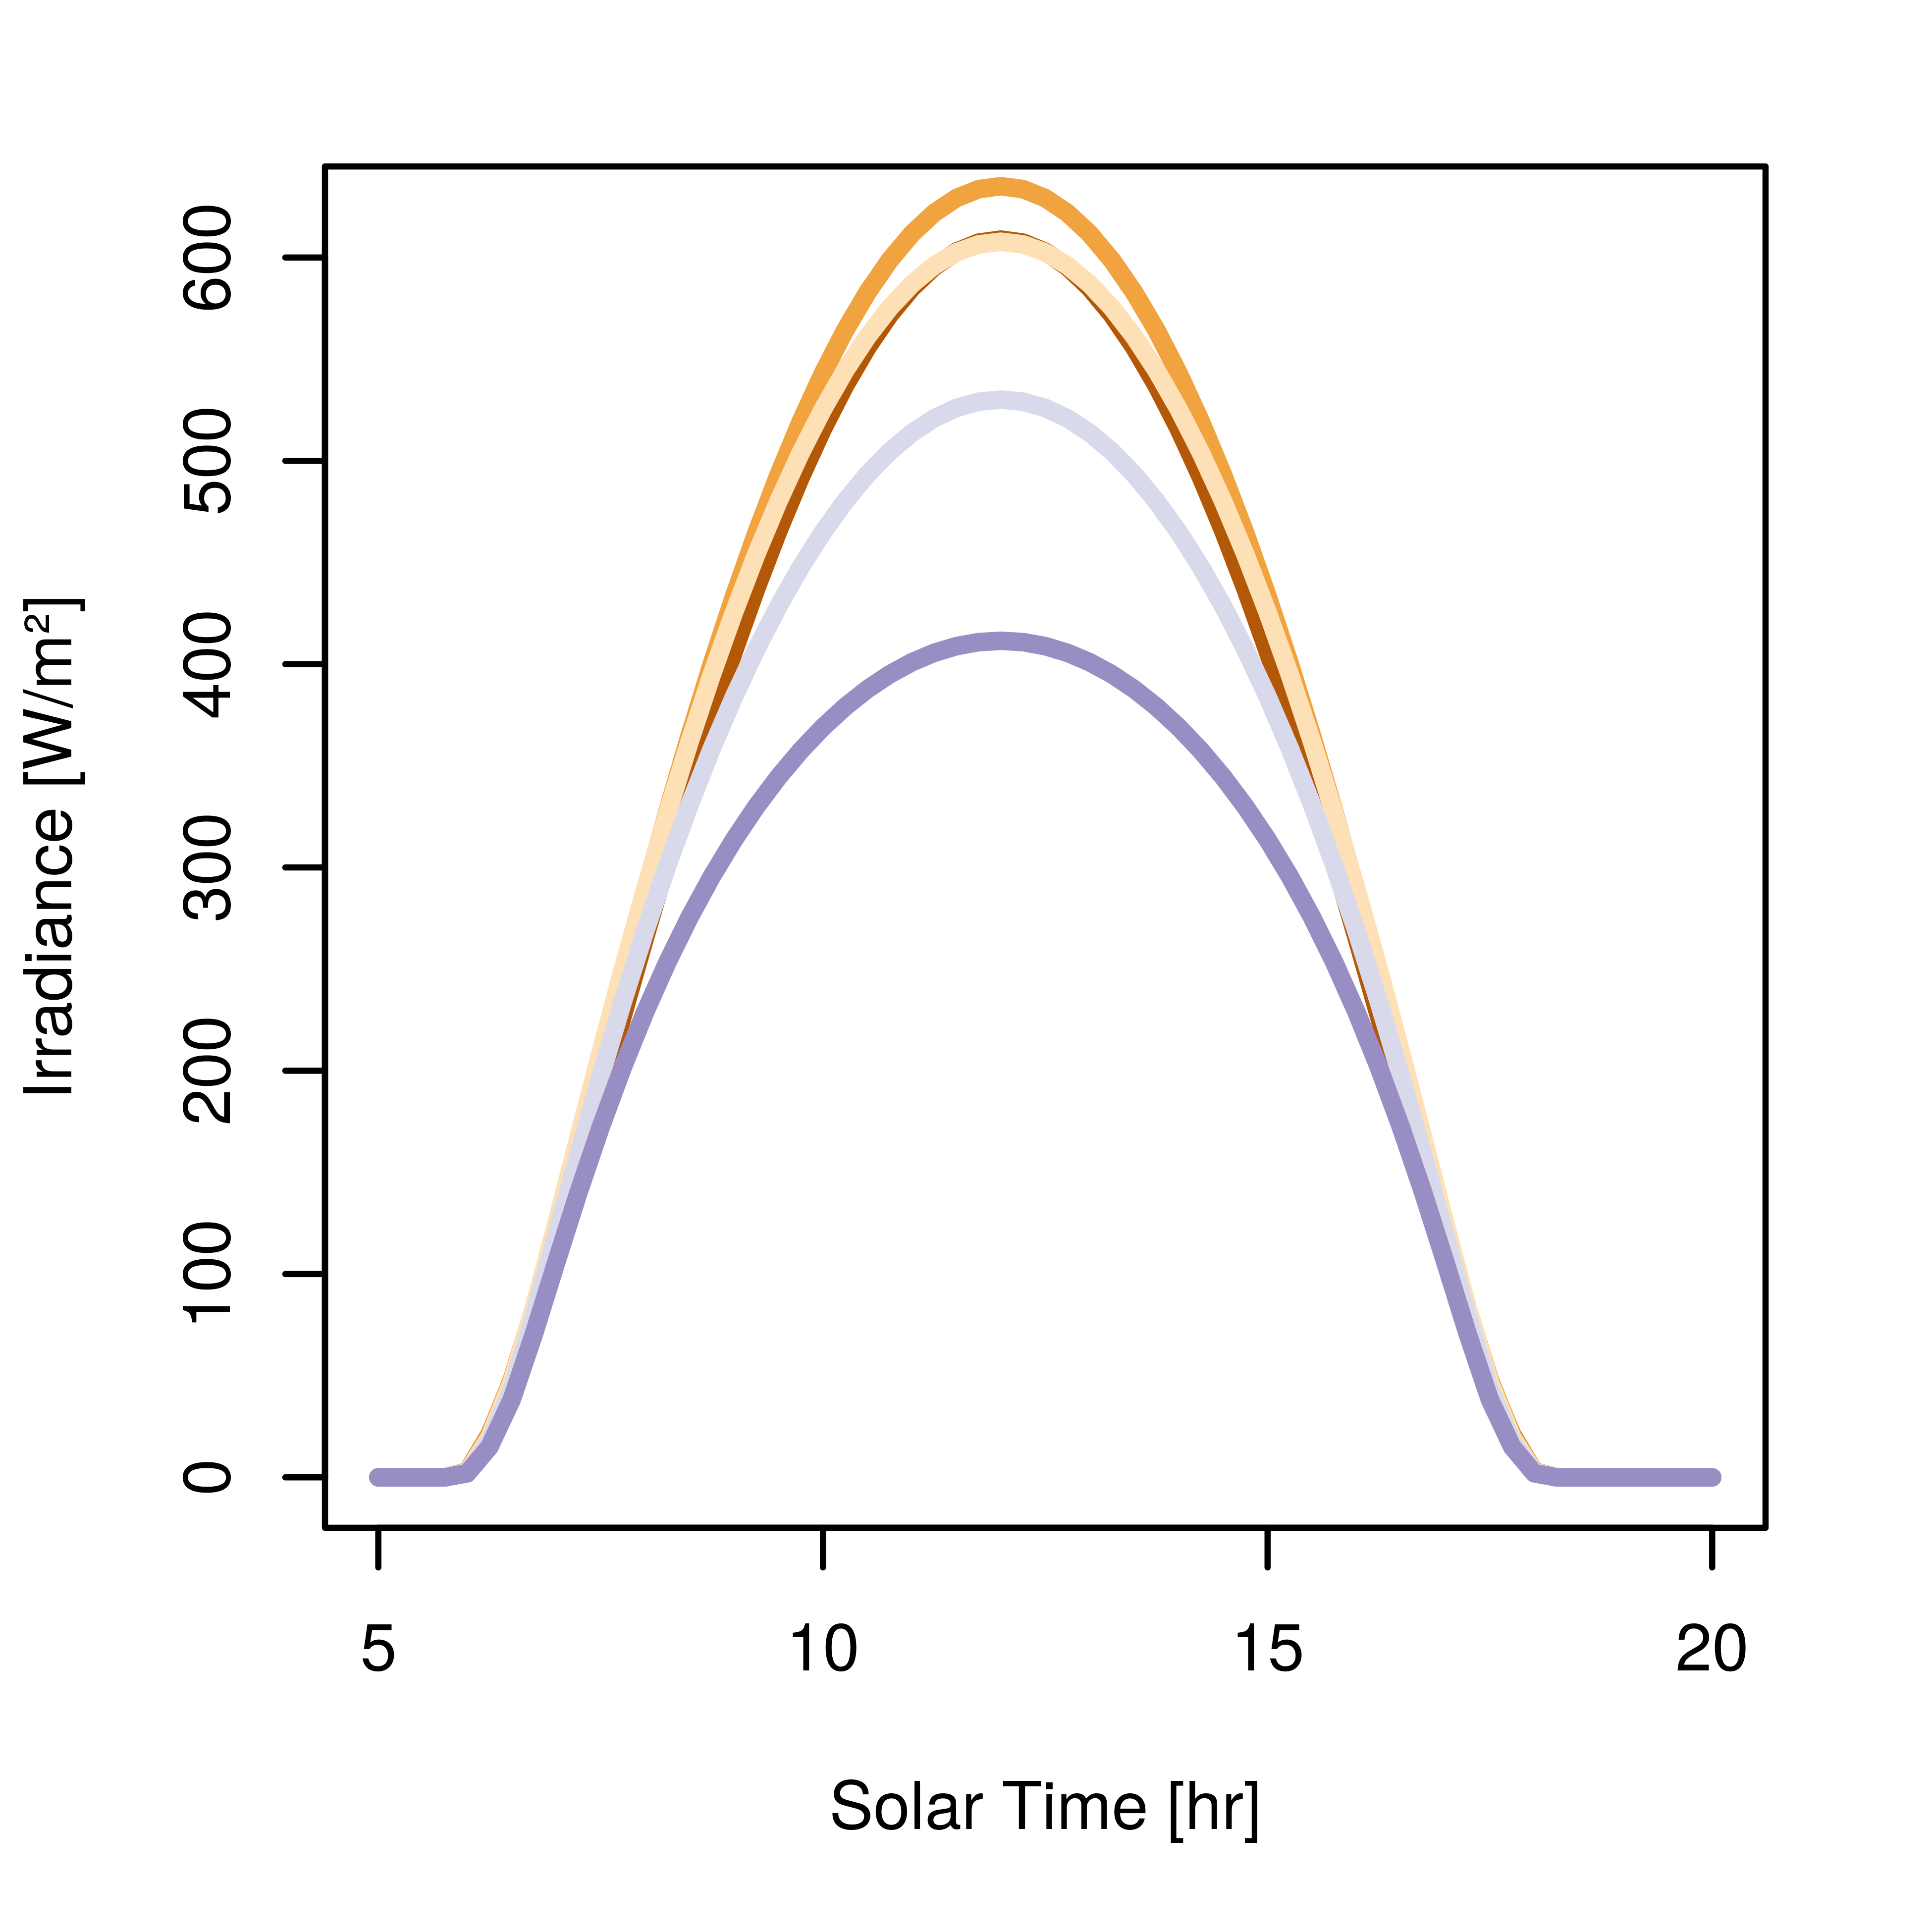
\includegraphics[height=\graphicsHeight]{sections/martian-environment/plots/gi-variation-1-for-ls-248-phi-2-tau-05-gammac-0-and-albedo-027.png}
  		\subcaption{$\gamma_{c} = \SI{0}{\degree}$ (South)}
  		\label{fig:sub:irradiance-inclined-gamma-c-0}
  	\end{subfigure}\hfill
    \begin{subfigure}[t]{\subfigureWidth}
      \centering
  		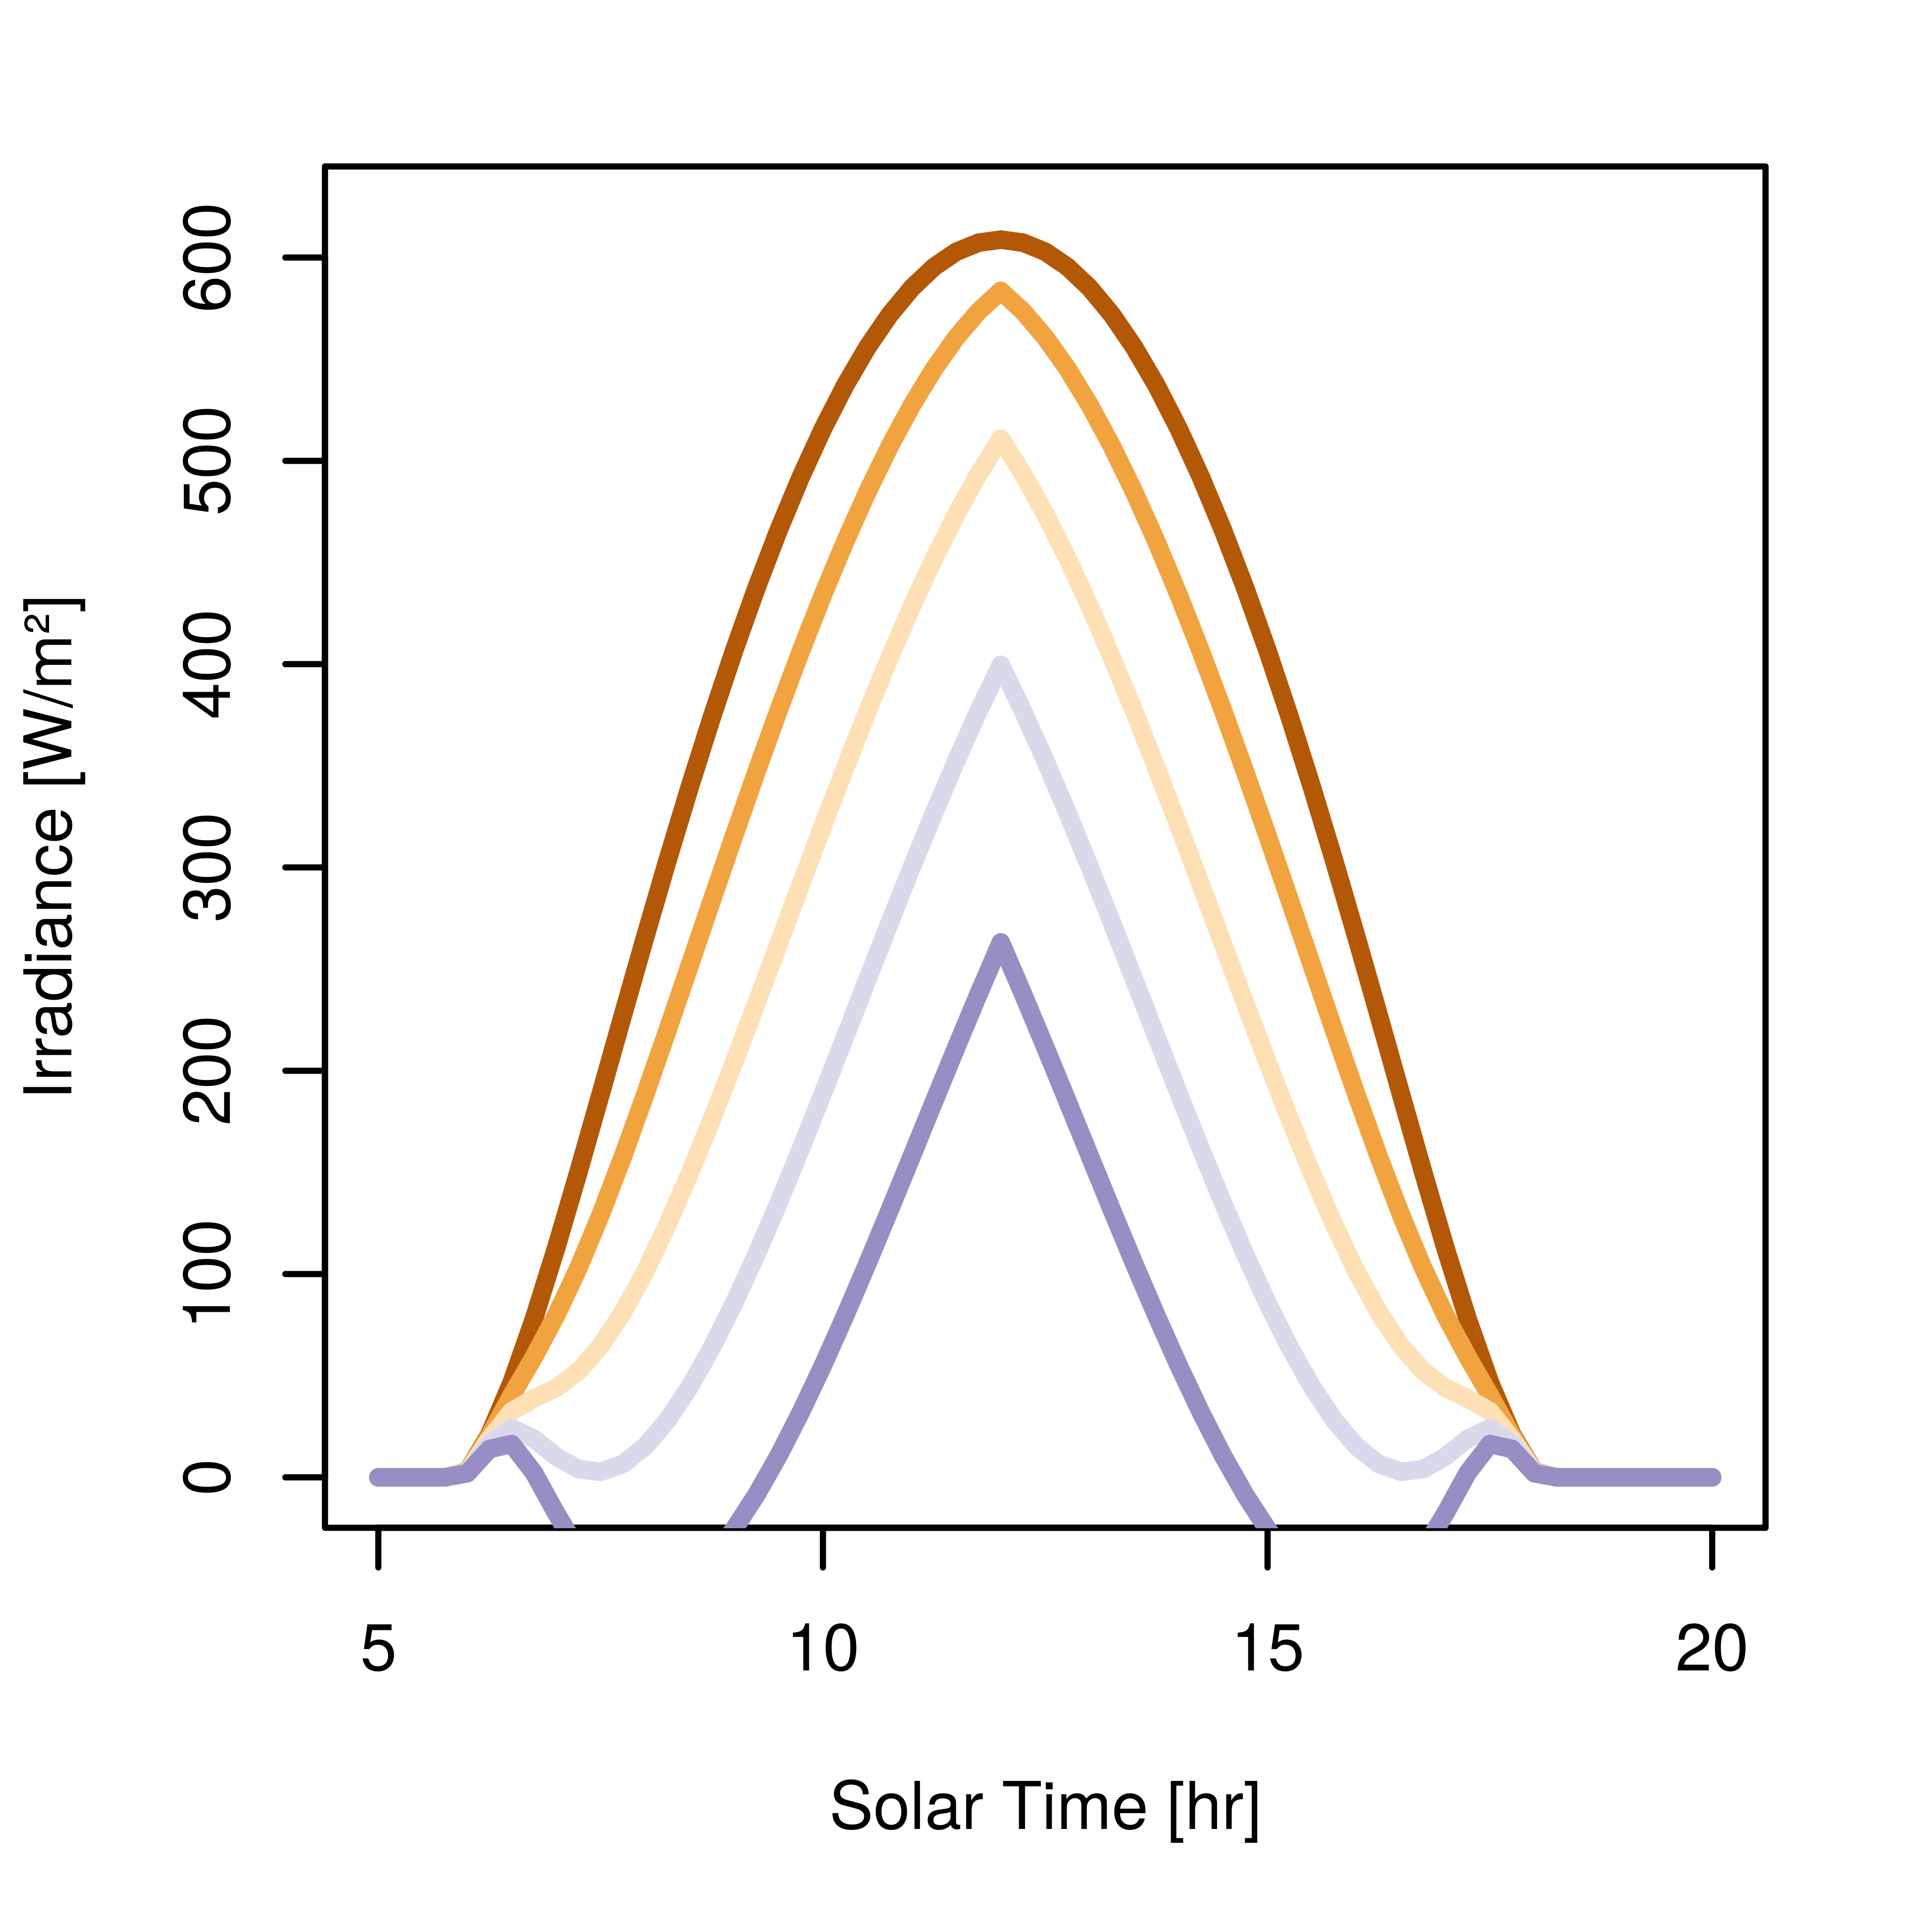
\includegraphics[height=\graphicsHeight]{sections/martian-environment/plots/gi-variation-2-for-ls-248-phi-2-tau-05-gammac-90-and-albedo-027.png}
  		\subcaption{$\gamma_{c} = \SI{-90}{\degree}$ (East)}
  		\label{fig:sub:irradiance-inclined-gamma-c-m90}
  	\end{subfigure}\\[0.8ex]
%% 2nd row
    \begin{subfigure}[t]{\subfigureWidth}
      \centering
  		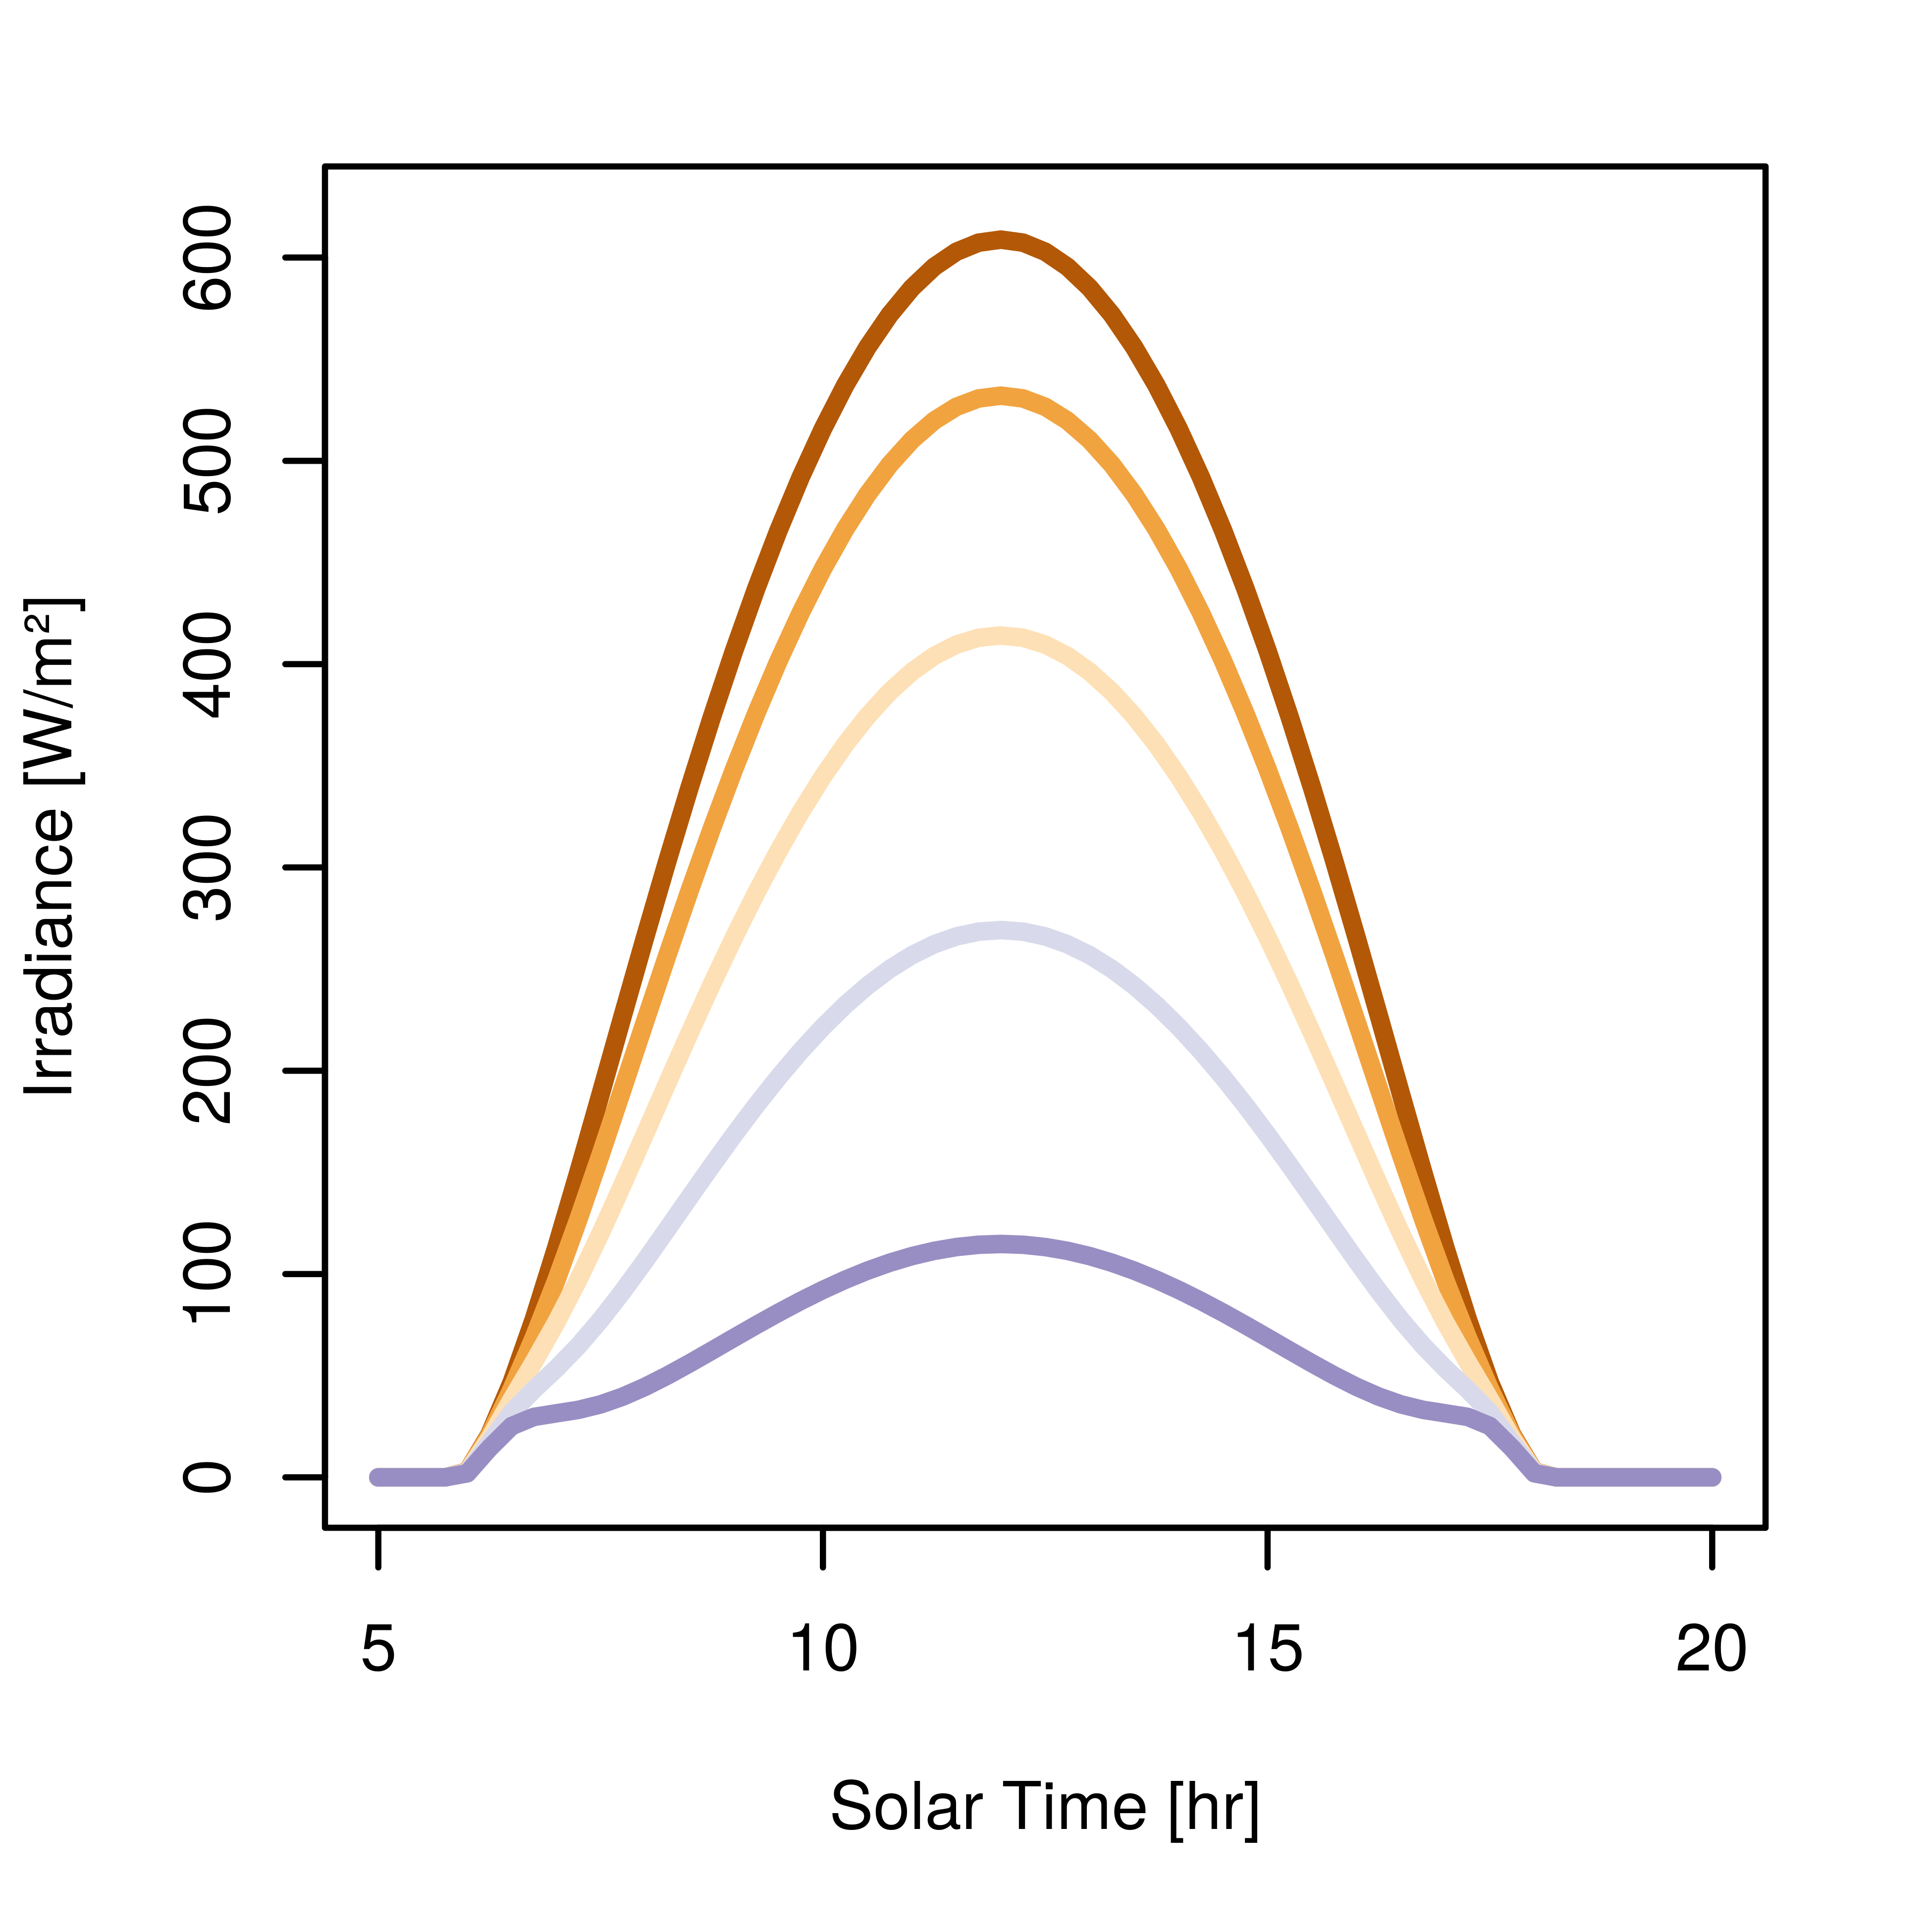
\includegraphics[height=\graphicsHeight]{sections/martian-environment/plots/gi-variation-3-for-ls-248-phi-2-tau-05-gammac-180-and-albedo-027.png}
  		\subcaption{$\gamma_{c} = \SI{-180}{\degree}$ (North)}
  		\label{fig:sub:irradiance-inclined-gamma-c-m180}
  	\end{subfigure}\hfill
	   \begin{subfigure}[t]{\subfigureWidth}
      \centering
  		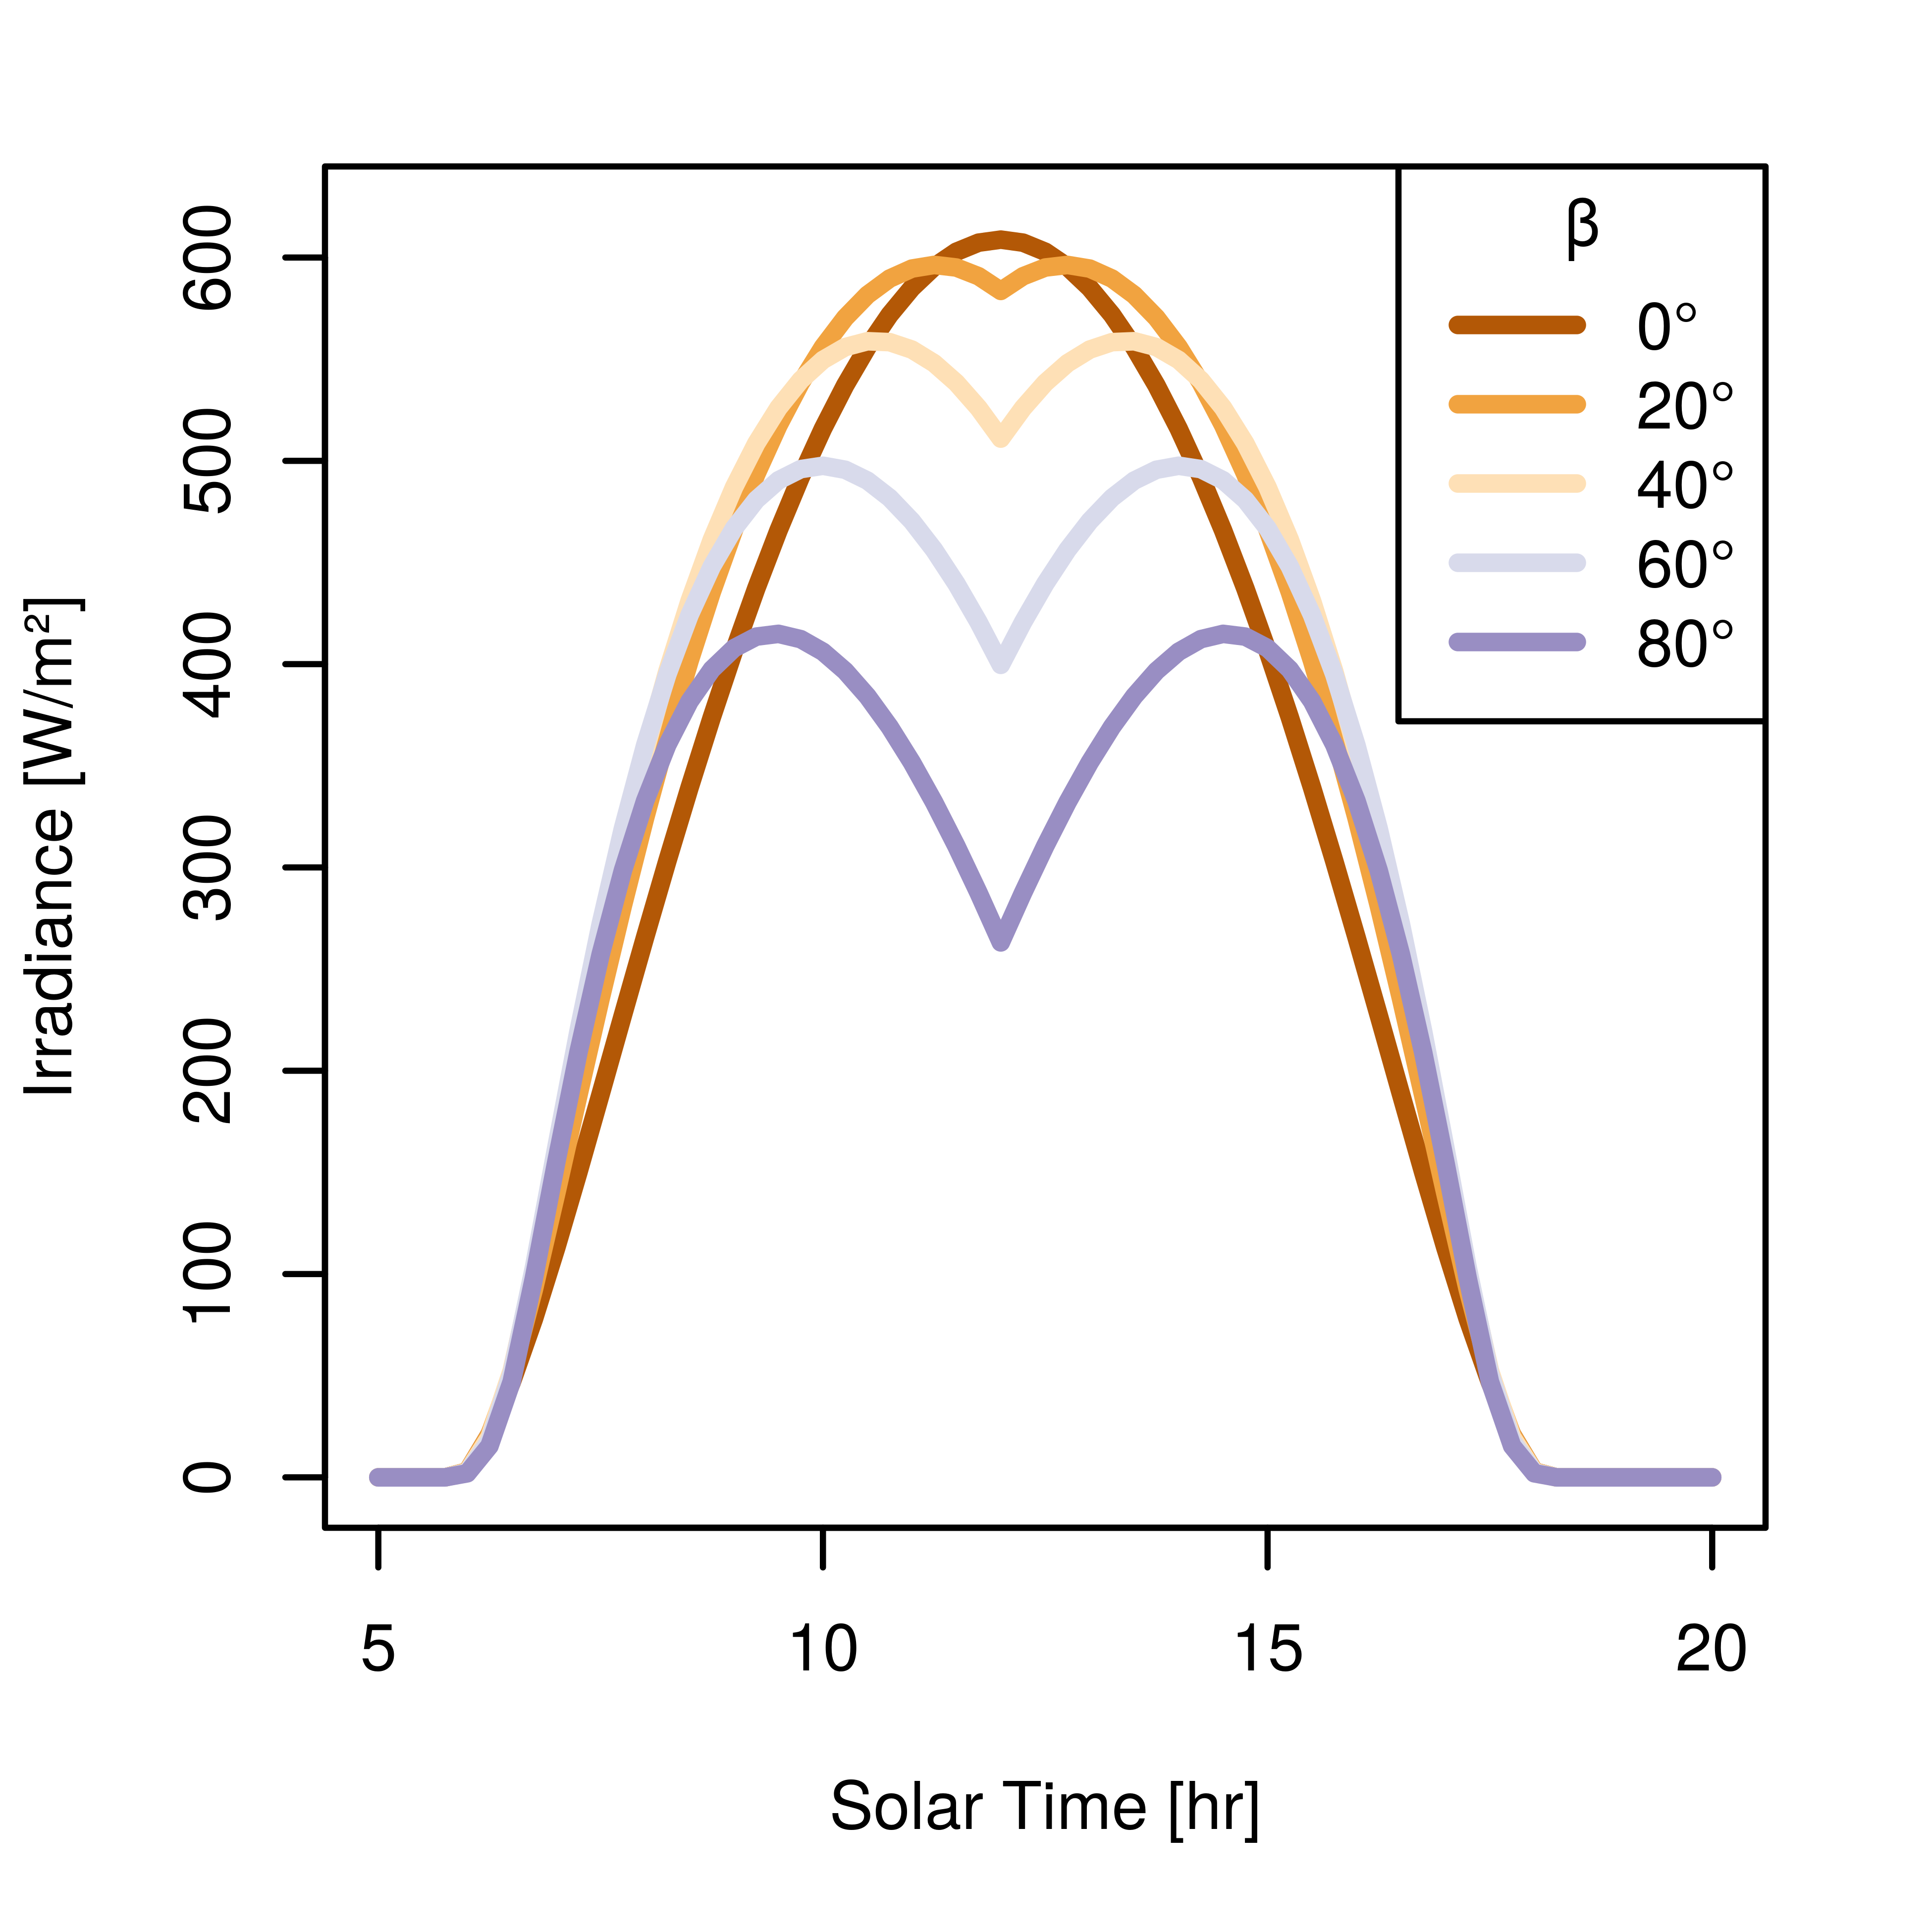
\includegraphics[height=\graphicsHeight]{sections/martian-environment/plots/gi-variation-4-for-ls-248-phi-2-tau-05-gammac-90-and-albedo-027.png}
  		\subcaption{$\gamma_{c} = \SI{90}{\degree}$ (West)}
  		\label{fig:sub:irradiance-inclined-gamma-c-90}
	   \end{subfigure}\hfill
	\caption{Diurnal variation of global irradiance on Mars inclined surface for different orientations when $L_{s} = \SI{248}{\degree}$, $\phi = \SI{-2}{\degree}$, and $\tau = \SI{0}{\degree}$.}
	\label{fig:plot:irradiance-inclined-gamma-c}
\vspace{-2ex}
\end{figure}

\subsubsection{Insolation}
\label{sec:MartianEnvironment:SolarRadiation:InclinedSurface:Insolation}

Insolations on an inclined surface are obtained by following the same procedure described in Section \ref{sec:MartianEnvironment:SolarRadiation:Insolation}. That is to say, integrating the $G_{\beta}$ irradiance Equation \ref{eq:G_beta} over a time period between $\omega_1$ and $\omega_2$.

\todo[inline]{TODO: Present plots for diurnal variation of global insolation on Mars inclined surface for different orientations. This is obtained by integrating the global irradiance on Mars incline surface.}

\todo[inline]{TODO: Emphasize that it doesn't matter which inclination and orientation configuration you have when most of the irradiance is scattered (dusty days).}
